% =====================================================================
%  Anatomía de un LLM — Fase VI — Módulo 25
%  Modelos sustitutos, diseño de experimentos y optimización bayesiana
%  Compilar: latexmk -r ../latexmkrc M25-optimizacion-bayesiana.tex
% =====================================================================
\documentclass[11pt,a4paper,twoside,openany]{book}
\usepackage{../estilo-apuntes}

\newcommand{\ApuntesCurso}{Anatomía de un LLM}
\newcommand{\ApuntesModulo}{Módulo 25}

% Notación propia del módulo
\newcommand{\X}{\mathcal{X}}
\newcommand{\D}{\mathcal{D}}
\newcommand{\GP}{\mathcal{GP}}
\newcommand{\N}{\mathcal{N}}
\newcommand{\EI}{\operatorname{EI}}
\newcommand{\PI}{\operatorname{PI}}
\newcommand{\LCB}{\operatorname{LCB}}
\newcommand{\UCB}{\operatorname{UCB}}
\newcommand{\HV}{\operatorname{HV}}
\newcommand{\Var}{\operatorname{Var}}
\newcommand{\Cov}{\operatorname{Cov}}
\newcommand{\tr}{\operatorname{tr}}
\newcommand{\diag}{\operatorname{diag}}
\newcommand{\fmejor}{f^{*}_{n}}
\newcommand{\Ky}{K_{y}}
\newcommand{\gwp}{\mathrm{GWP}}
\declaretheorem[style=defin,name=Algoritmo,sibling=definicion]{algoritmo}
\crefname{algoritmo}{algoritmo}{algoritmos}
\crefname{figure}{figura}{figuras}
\crefname{table}{tabla}{tablas}
\makeatletter\g@addto@macro\UrlBreaks{\do\-\do\/}\makeatother

\hypersetup{pdftitle={Módulo 25. Modelos sustitutos, diseño de experimentos y optimización bayesiana},pdfauthor={Anatomía de un LLM}}

\begin{document}
\frontmatter
% ------------------------------------------------------------------ Portada
\begin{titlepage}
\centering
\vspace*{2.5cm}
{\large\scshape Anatomía de un LLM}\par
\vspace{0.4cm}
{\normalsize Fundamentos matemáticos de los modelos de lenguaje}\par
\vspace{2.2cm}
\rule{\textwidth}{0.8pt}\par\vspace{0.5cm}
{\small\scshape Fase VI \textperiodcentered\ Diseño y construcción de optimizadores con IA}\par\vspace{0.3cm}
{\Huge\bfseries Módulo 25\par}\vspace{0.3cm}
{\LARGE Modelos sustitutos, diseño de experimentos\\[2pt] y optimización bayesiana\par}
\vspace{0.2cm}
{\large Cómo optimizar procesos caros y ruidosos con pocos experimentos\par}
\vspace{0.5cm}\rule{\textwidth}{0.4pt}\par
\vspace{1.6cm}
{\large Apuntes del curso}\par
\vfill
{\small Edición de octubre de 2026}\par
\end{titlepage}

% ------------------------------------------------------- Presentación
\chapter*{Presentación del módulo}
\addcontentsline{toc}{chapter}{Presentación del módulo}
\markboth{Presentación del módulo}{}

Muchos problemas de optimización de la industria no se parecen al entrenamiento de una red neuronal. No hay gradiente, cada evaluación cuesta horas de máquina, material o semanas de espera, y el resultado llega con ruido. Ajustar una inyectora de plástico, formular un hormigón o elegir los hiperparámetros de un modelo son problemas de este tipo: se dispone de un presupuesto de unas decenas de experimentos y hay que gastarlo bien. Este módulo estudia el conjunto de técnicas que la estadística y el aprendizaje automático han desarrollado para ello: el diseño de experimentos clásico, que decide qué ensayos hacer antes de ver ningún resultado; los modelos sustitutos, que aprenden una aproximación barata del proceso con su incertidumbre; y la optimización bayesiana, que usa esa incertidumbre para elegir, uno a uno o por lotes, los siguientes experimentos. El ajuste de hiperparámetros de los modelos de aprendizaje automático, incluidos los LLM, aparece como un caso particular, con métodos propios que aprovechan evaluaciones parciales más baratas.

\section*{Objetivos}
Al finalizar el módulo, el estudiante debe ser capaz de:
\begin{enumerate}[label=\arabic*.]
  \item formular un problema de optimización de caja negra con presupuesto, ruido y restricciones, y elegir una medida de rendimiento adecuada (regret simple o acumulado);
  \item diseñar y analizar experimentos factoriales completos y fraccionados, ajustar superficies de respuesta y construir hipercubos latinos, justificando sus propiedades;
  \item construir modelos sustitutos (polinomios, procesos gaussianos y \emph{ensembles} de redes), ajustar sus hiperparámetros por verosimilitud marginal y validarlos;
  \item deducir la forma cerrada de la mejora esperada, comparar las funciones de adquisición habituales y extenderlas a restricciones, lotes, varios objetivos y varias fidelidades;
  \item diseñar de principio a fin un optimizador para un proceso industrial real, desde las variables y el presupuesto hasta los ensayos de confirmación;
  \item ajustar hiperparámetros con búsqueda aleatoria, TPE y Hyperband, y decidir cuándo dejar de experimentar.
\end{enumerate}

\section*{Requisitos previos}
Se reutilizan los siguientes contenidos del curso. Del módulo~0.6, la integral gaussiana (§4.5) y la integración por partes (§3.2); del módulo~0.7, el criterio del hessiano y los multiplicadores de Lagrange (§5.2 y §5.4); del módulo~0.8, la distribución normal y la tipificación (§6.3); del módulo~0.9, la varianza muestral (§2.5), las distribuciones $\chi^2$ y $t$ (§3.4), los intervalos de confianza (§4.3), el contraste de hipótesis y el $p$-valor (§5.1–§5.3) y la recta de mínimos cuadrados (§6.1). Del módulo~3, el teorema espectral para matrices simétricas (§3.3); del módulo~4, el gradiente (§1.2) y la clasificación de puntos críticos (§4.3); del módulo~5, la distribución normal (§3.3), la máxima verosimilitud (§4.2), la inferencia bayesiana (§4.4) y el método de Monte Carlo (§5.3); del módulo~7, el descenso de gradiente y Adam (temas~2 y~5); del módulo~8, las ecuaciones normales (§2.2), la interpretación probabilística de la regresión (§2.5), la descomposición sesgo-varianza (§5.2), la regresión ridge y su interpretación bayesiana (§6.1 y §6.2) y la validación cruzada (§6.5); del módulo~9, el perceptrón multicapa (tema~1); y del módulo~10, la diferenciación automática en modo inverso (tema~3), que se usa en las redes informadas por la física.

\section*{Organización}
\begin{center}\small
\begin{tabular}{@{}cll@{}}
\toprule
Tema & Contenido & Fuentes principales \\
\midrule
1 & Optimizar procesos caros y ruidosos & \cite{garnett}, \cite{frazier}, \cite{kw}, \cite{mn} \\
2 & Diseño de experimentos & \cite{montgomery}, \cite{psu503}, \cite{mckay}, \cite{boxwilson} \\
3 & Modelos sustitutos & \cite{rw}, \cite{garnett}, \cite{lakshmi}, \cite{raissi} \\
4 & Optimización bayesiana & \cite{jones}, \cite{frazier}, \cite{garnett}, \cite{srinivas} \\
5 & Casos de estudio: moldeo por inyección y hormigón & \cite{fernandes}, \cite{ament}, \cite{shields} \\
6 & Hiperparámetros, AutoML, validación y parada & \cite{feurer}, \cite{bergstra12}, \cite{tpe}, \cite{hyperband} \\
\bottomrule
\end{tabular}
\end{center}

Cada tema combina teoría formal, al menos un caso de estudio desarrollado con datos numéricos, una tabla de tecnologías y una observación sobre los errores más frecuentes en la práctica. Termina con una lista de lecturas y con ejercicios graduados en tres niveles: $\star$ comprensión, $\star\star$ formulación y cálculo a mano, y $\star\star\star$ demostración o diseño razonado. Los ejercicios marcados con \emph{Fuente} están adaptados de cursos y libros de texto universitarios; el enunciado se ha redactado de nuevo y los datos se han cambiado para que puedan resolverse a mano. Las soluciones completas, paso a paso, están en el \cref{ap:soluciones}. El cuaderno \texttt{M25-practica.ipynb} implementa todos los casos de estudio; las cifras que en el texto se atribuyen a «la práctica» proceden de su ejecución con las semillas fijadas en él.

\section*{Sobre las fuentes}
El texto es de redacción propia. La formulación del problema y la optimización bayesiana siguen el libro de Garnett~\cite{garnett}, el tutorial de Frazier~\cite{frazier} y la revisión de Shahriari \emph{et al.}~\cite{shahriari}; la mejora esperada se toma del artículo original de Jones, Schonlau y Welch~\cite{jones}. Los procesos gaussianos siguen los capítulos~2, 4 y~5 de Rasmussen y Williams~\cite{rw} y la tarea~1 del curso 4F13 de Cambridge~\cite{cam4f13}. El diseño de experimentos sigue a Montgomery~\cite{montgomery} y el curso STAT~503 de Penn State~\cite{psu503}; el hipercubo latino, a McKay, Beckman y Conover~\cite{mckay}. Los planes de muestreo y los sustitutos siguen además los capítulos~13 a~16 de Kochenderfer y Wheeler~\cite{kw}, texto del curso AA222/CS361 de Stanford~\cite{aa222}, y el capítulo~10 de Martins y Ning~\cite{mn}. El ajuste de hiperparámetros sigue el capítulo~1 del libro de AutoML de Hutter, Kotthoff y Vanschoren~\cite{feurer} y los artículos originales de cada método. Las aplicaciones industriales citadas (centros de datos de Google, AlphaGo, hormigón de bajo carbono, química de síntesis) proceden exclusivamente de publicaciones y comunicados públicos; los datos de los casos de estudio de los temas~1 a~5 son sintéticos, generados por simuladores escritos para el curso con órdenes de magnitud plausibles, y se indica así cada vez.

\section*{Notación}
\begin{center}\small
\begin{tabularx}{\textwidth}{@{}l>{\raggedright\arraybackslash}X@{}}
\toprule
Símbolo & Significado \\
\midrule
$x\in\X\subset\R^{d}$ & vector de variables de decisión (parámetros del proceso) en el dominio $\X$ \\
$f(x)$, $y=f(x)+\varepsilon$ & función objetivo (a minimizar) y observación con ruido $\varepsilon\sim\N(0,\sigma_n^2)$ \\
$c_j(x)\le 0$ & restricciones \\
$\D_n=\{(x_i,y_i)\}_{i=1}^{n}$ & datos tras $n$ evaluaciones; $N$ es el presupuesto total \\
$u\in[-1,1]^{d}$ & variables codificadas de un diseño de experimentos \\
$k(x,x')$, $K$, $\Ky=K+\sigma_n^2 I$ & núcleo (covarianza), matriz de Gram y matriz con ruido \\
$\ell$, $\sigma_f^2$, $\theta$ & longitud de escala, varianza de la señal y vector de hiperparámetros \\
$\mu_n(x)$, $\sigma_n(x)$ & media y desviación típica posteriores de $f(x)$ dados $\D_n$ \\
$\fmejor$ & mejor valor (mínimo) de referencia tras $n$ evaluaciones \\
$\varphi$, $\Phi$ & densidad y función de distribución de la normal estándar \\
$\alpha_n(x)$ & función de adquisición; $\EI$, $\PI$, $\LCB$ sus casos principales \\
$r_N=f(\hat x_N)-f(x^\star)$ & regret simple de la recomendación $\hat x_N$ \\
$\lambda$, $\Lambda$ & configuración de hiperparámetros y espacio de configuraciones \\
\bottomrule
\end{tabularx}
\end{center}

\tableofcontents

\mainmatter
% =====================================================================
\chapter{Optimizar procesos caros y ruidosos}
\label{tema:1}
% =====================================================================

Este tema plantea el problema común a todo el módulo: minimizar una función que solo se conoce a través de experimentos caros y ruidosos, con un presupuesto fijo de evaluaciones y con restricciones que a veces tampoco se conocen de antemano. La formalización sigue el capítulo~1 de Garnett~\cite{garnett} y la sección~2 del tutorial de Frazier~\cite{frazier}; la discusión sobre cuándo compensa un modelo sustituto sigue la §10.1 de Martins y Ning~\cite{mn}, y los planes de muestreo en rejilla, la §13.1 de Kochenderfer y Wheeler~\cite{kw}.

\section{El problema de la caja negra}

En el entrenamiento de una red (módulo~7) la función objetivo es una fórmula explícita, su gradiente se obtiene por diferenciación automática (módulo~10) y evaluarla en un minilote cuesta milisegundos. En un proceso industrial nada de esto se cumple: para conocer la tasa de defectos de una inyectora con un ajuste dado hay que fabricar un lote de piezas e inspeccionarlo.

\begin{definicion}[Problema de optimización de caja negra]\label{def:cajanegra}
Sean $\X\subset\R^{d}$ un dominio compacto (habitualmente un hiperrectángulo $\prod_{j}[a_j,b_j]$), $f\colon\X\to\R$ una función desconocida y $N\in\mathbb{N}$ un \emph{presupuesto} de evaluaciones. Un \emph{oráculo} devuelve, para cada $x\in\X$ elegido, una observación
\[
y=f(x)+\varepsilon,\qquad \E[\varepsilon]=0,\quad \Var(\varepsilon)=\sigma_n^2(x),
\]
con ruidos independientes entre evaluaciones. Una \emph{política} elige secuencialmente $x_{n+1}$ a partir de los datos $\D_n=\{(x_i,y_i)\}_{i\le n}$ y, agotado el presupuesto, emite una \emph{recomendación} $\hat x_N\in\X$. El objetivo es que $f(\hat x_N)$ sea lo más próximo posible a $\min_{x\in\X}f(x)$.
\end{definicion}

Tres rasgos distinguen este problema de los de los módulos~7 y~8: no hay gradiente (ni siquiera ruidoso), el número de evaluaciones es pequeño (de diez a unos centenares) y el coste de decidir dónde evaluar es despreciable frente al de evaluar. Esta última asimetría justifica gastar mucho cómputo en cada decisión: ajustar un modelo estadístico de $f$ y optimizar sobre él~\cite[§1.1]{garnett}.

\begin{definicion}[Regret]\label{def:regret}
Sea $x^\star\in\arg\min_{\X}f$. El \emph{regret simple} de la recomendación es $r_N=f(\hat x_N)-f(x^\star)\ge 0$. El \emph{regret acumulado} de las evaluaciones es $R_N=\sum_{n=1}^{N}\bigl(f(x_n)-f(x^\star)\bigr)$.
\end{definicion}

La elección entre ambos depende del caso. En un estudio de laboratorio solo importa la receta final: se mide $r_N$. Si los experimentos se hacen en la línea de producción y las piezas ensayadas se venden o se desechan, cada experimento malo cuesta dinero y se mide $R_N$; Garnett~\cite[§6.1–6.2]{garnett} formaliza ambas utilidades.

\begin{observacion}
La recomendación $\hat x_N$ no tiene por qué ser uno de los puntos evaluados ni el de mejor observación. Con ruido, el mínimo observado es un mal estimador del mínimo verdadero (\cref{prop:ganador}); en la práctica se recomienda el punto que minimiza un modelo ajustado a todos los datos y se confirma con ensayos repetidos.
\end{observacion}

\section{Presupuesto y ruido}

\begin{proposicion}[Maldición de la dimensión para rejillas]\label{prop:rejilla}
Sea $\X=[0,1]^{d}$ y sea $h\in(0,\tfrac12]$. Si un conjunto de $N$ puntos garantiza que todo $x\in\X$ dista menos de $h$ en norma del máximo de algún punto del conjunto, entonces $N\ge(2h)^{-d}$. Una rejilla de $m$ niveles por variable tiene $m^{d}$ puntos.
\end{proposicion}

\begin{proof}
La bola de radio $h$ en norma del máximo es un cubo de lado $2h$ y volumen $(2h)^{d}$. Si las $N$ bolas recubren $\X$, la suma de sus volúmenes es al menos el de $\X$, que vale~1: $N(2h)^{d}\ge 1$. La segunda afirmación es la regla del producto (módulo~0.8, §1.1).
\end{proof}

Con $h=0{,}1$ (un décimo del rango de cada variable) hacen falta al menos $5^{d}$ puntos: 125 con tres variables y casi diez millones con diez. Ningún proceso físico admite ese presupuesto; de ahí la necesidad de diseños que no crezcan exponencialmente (\cref{tema:2}) y de modelos que interpolen entre ensayos (\cref{tema:3}).

El ruido tiene dos orígenes: la variabilidad del proceso (lote de materia prima, temperatura ambiente, desgaste) y el error de medida. Cuando la respuesta es una proporción estimada con $m$ piezas, el ruido es binomial.

\begin{proposicion}\label{prop:binomial}
Si en un lote de $m$ piezas cada una es defectuosa con probabilidad $d$, independientemente, la fracción observada $\hat d$ cumple $\E[\hat d]=d$ y $\Var(\hat d)=d(1-d)/m$.
\end{proposicion}

\begin{proof}
El número de defectuosas es binomial $B(m,d)$, de media $md$ y varianza $md(1-d)$ (módulo~0.8, §5.4); al dividir por $m$, la media se divide por $m$ y la varianza por $m^{2}$.
\end{proof}

La consecuencia más traicionera del ruido es que el mejor resultado observado es sistemáticamente optimista.

\begin{proposicion}[Maldición del ganador]\label{prop:ganador}
Sean $y_i=f(x_i)+\varepsilon_i$, $i=1,\dots,n$, con $\varepsilon_i$ independientes de media nula. Entonces
\[
\E\Bigl[\min_{i}y_i\Bigr]\le\min_{i}f(x_i).
\]
Si además todos los $f(x_i)$ son iguales a $f_0$ y $\varepsilon_i\sim\N(0,\sigma^2)$, entonces $\E[\min_i y_i]=f_0-\sigma\,e_n$, con $e_n=\E[\max_i Z_i]$ para $Z_i\sim\N(0,1)$ independientes.
\end{proposicion}

\begin{proof}
Sea $j$ un índice con $f(x_j)=\min_i f(x_i)$. Como $\min_i y_i\le y_j$ siempre, tomando esperanzas $\E[\min_i y_i]\le\E[y_j]=f(x_j)$. Para la segunda parte, $\min_i(f_0+\sigma Z_i)=f_0-\sigma\max_i(-Z_i)$, y $(-Z_i)$ tiene la misma distribución que $(Z_i)$.
\end{proof}

Los valores de $e_n$ se obtienen por integración numérica: $e_2=1/\sqrt\pi\approx 0{,}5642$ (\cref{eje:1-max2}), $e_5\approx 1{,}163$, $e_{10}\approx 1{,}539$ y $e_{30}\approx 2{,}043$. Elegir el mejor de diez ensayos igual de buenos produce un resultado aparentemente mejor en más de 1,5 desviaciones típicas.

\section{Restricciones}

Las restricciones de un proceso son de naturaleza muy distinta, y conviene clasificarlas antes de elegir el método~\cite[§11.2]{garnett}, \cite[§1.4]{kw}:
\begin{itemize}
  \item \emph{conocidas y baratas}: los límites de la máquina, la suma de las fracciones de una mezcla igual a~1, una relación entre variables. Se imponen directamente al generar candidatos;
  \item \emph{desconocidas y caras}: una especificación de calidad que solo se comprueba con el experimento (alabeo máximo, resistencia mínima). Se modelan igual que el objetivo y se trata su probabilidad de cumplirse (\cref{tema:4});
  \item \emph{ocultas}: zonas donde el experimento falla y no produce dato (la pieza sale incompleta, la simulación no converge). Se modelan como una clasificación;
  \item \emph{de seguridad}: no basta con acabar en un punto factible, sino que no se debe \emph{ensayar} un punto peligroso (presión excesiva, temperatura de degradación del polímero). Exigen métodos de exploración segura~\cite[§16.6]{kw}.
\end{itemize}

\begin{definicion}[Problema con restricciones de caja negra]\label{def:restricciones}
Se busca $\min_{x\in\X}f(x)$ sujeto a $c_j(x)\le 0$, $j=1,\dots,J$, donde cada $c_j$ es una función desconocida que se observa con ruido en el mismo experimento que $f$ o en uno distinto. El regret simple se define respecto al mejor punto \emph{factible}, y una recomendación no factible se considera un fracaso, sea cual sea su valor de $f$.
\end{definicion}

\section{El bucle de optimización con un modelo sustituto}

Todos los métodos del módulo comparten la estructura de la \cref{fig:bucle}. Un diseño inicial (\cref{tema:2}) proporciona los primeros datos; un modelo sustituto (\cref{tema:3}) resume lo aprendido con su incertidumbre; una función de adquisición (\cref{tema:4}) traduce el modelo en la decisión del siguiente experimento; y una regla de parada (\cref{tema:6}) decide cuándo dejar de experimentar.

\begin{figure}[ht]
\centering
\begin{tikzpicture}[font=\small,>={Stealth[length=2mm]},
  caja/.style={draw,rounded corners,align=center,minimum width=2.6cm,minimum height=1cm,thick}]
  \node[caja] (doe) at (0,0) {diseño inicial\\(LHS, factorial)};
  \node[caja] (exp) at (4.2,0) {experimento\\$y=f(x)+\varepsilon$};
  \node[caja] (mod) at (8.4,0) {modelo sustituto\\$\mu_n,\ \sigma_n$};
  \node[caja] (acq) at (8.4,-2.4) {adquisición\\$x_{n+1}=\arg\max\alpha_n$};
  \node[caja] (par) at (4.2,-2.4) {¿parar?};
  \node[caja] (rec) at (0,-2.4) {recomendación $\hat x_N$\\y confirmación};
  \draw[->,thick] (doe) -- (exp);
  \draw[->,thick] (exp) -- node[above]{$\D_n$} (mod);
  \draw[->,thick] (mod) -- (acq);
  \draw[->,thick] (acq) -- (par);
  \draw[->,thick] (par) -- node[right]{no} (exp);
  \draw[->,thick] (par) -- node[above]{sí} (rec);
\end{tikzpicture}
\caption{El bucle de optimización con modelo sustituto. El coste está en la caja «experimento»; todas las demás son cálculos baratos.}
\label{fig:bucle}
\end{figure}

\begin{table}[ht]
\centering\small
\begin{tabularx}{\textwidth}{@{}>{\raggedright\arraybackslash}p{2.9cm}>{\raggedright\arraybackslash}X>{\raggedright\arraybackslash}p{3.6cm}@{}}
\toprule
Familia & Cuándo es adecuada & Limitaciones \\
\midrule
Rejilla y un factor cada vez & Una o dos variables, evaluaciones baratas & Crece como $m^{d}$; no detecta interacciones \\
Diseño de experimentos y superficie de respuesta & 2–8 variables, decenas de ensayos, se quiere entender el proceso & Modelo polinómico local \\
Optimización bayesiana & 1–20 variables, 10–500 evaluaciones caras y ruidosas & Coste cúbico en $n$; peor en dimensión alta \\
Evolutivos (CMA-ES, genéticos) & Miles de evaluaciones baratas, paisajes irregulares & Poco eficientes en número de evaluaciones \\
Gradiente (adjunto, autodiferenciación) & Simuladores diferenciables, muchas variables & Requiere acceso al código del modelo \\
\bottomrule
\end{tabularx}
\caption{Familias de métodos según el presupuesto y la dimensión. El límite de unas veinte variables para la optimización bayesiana procede de Frazier~\cite[§1]{frazier}.}
\label{tab:familias}
\end{table}

La §10.1 de Martins y Ning~\cite{mn} resume el criterio económico: un sustituto compensa cuando el coste de construirlo y consultarlo es pequeño frente al de las evaluaciones que ahorra, cuando el ruido impide usar diferencias finitas y cuando se quiere reutilizar el modelo para otras preguntas (sensibilidad, robustez).

\section{Caso de estudio: ajuste de una inyectora}

\begin{ejemplo}[Formulación del ajuste de un proceso de moldeo por inyección]\label{ej:inyectora}
Una inyectora fabrica una carcasa de polipropileno. Tras revisar la literatura del proceso~\cite{fernandes}, se eligen tres variables: temperatura de fusión $T\in[200,260]$~°C, presión de mantenimiento $P\in[30,90]$~MPa y tiempo de enfriamiento $t_e\in[8,30]$~s. Los datos de este caso son sintéticos: proceden de un simulador escrito para el curso (Parte~1 de la práctica), con mecanismos de defecto plausibles (rechupes si falta presión o enfriamiento, rebabas si sobran presión y temperatura, piezas incompletas si el material está frío).

\emph{Objetivo.} El tiempo de ciclo es conocido, $t_c(x)=8+t_e+0{,}05\,(T-200)$~s, y la fracción defectuosa $d(x)$ es desconocida. Con un coste de máquina de $45$~€/h y un coste de material de $0{,}40$~€ por pieza, el coste por pieza \emph{buena} es
\[
C(x)=\frac{45\,t_c(x)/3600+0{,}40}{1-d(x)}\quad\text{€}.
\]
\emph{Restricción de calidad.} El alabeo medio $w(x)$ no debe superar $0{,}45$~mm.

\emph{Experimento.} Cada ensayo es un lote de $m=200$ piezas tras estabilizar la máquina; se cuentan las defectuosas y se mide el alabeo de 20 piezas. Con unos 30~s por ciclo, el lote ocupa la máquina 100 minutos y, con el cambio de ajuste y la estabilización, unas dos horas.

\emph{La receta actual.} El operario trabaja con $x_0=(240,50,26)$: $t_c=8+26+0{,}05\cdot 40=36$~s, $d=2{,}17\,\%$ y
\[
C(x_0)=\frac{45\cdot 36/3600+0{,}40}{1-0{,}0217}=\frac{0{,}85}{0{,}9783}=0{,}8688\ \text{€}.
\]
\emph{El óptimo} (que solo se conoce porque el simulador es nuestro) está en $x^\star=(213{,}5;\ 70{,}5;\ 18{,}5)$, con $t_c=27{,}18$~s, $d=4{,}95\,\%$, $w=0{,}450$~mm y $C(x^\star)=0{,}7398/0{,}9505=0{,}7782$~€: un ahorro del $10{,}4\,\%$, unos $90\,600$~€ al año por cada millón de piezas. El óptimo acepta más defectos a cambio de un ciclo nueve segundos más corto, y la restricción de alabeo está activa: es ella la que fija el tiempo de enfriamiento.

\emph{Presupuesto y ruido.} Una rejilla de 5 niveles exigiría $5^{3}=125$ lotes, unas 250 horas de máquina. Se dispone de 30 lotes. En el óptimo, por la \cref{prop:binomial}, $\sqrt{0{,}0495\cdot0{,}9505/200}=0{,}0153$: la fracción defectuosa se mide con una desviación de $1{,}5$ puntos porcentuales, que se traduce en una desviación de $0{,}0126$~€ en el coste. Por la \cref{prop:ganador}, el mejor de diez lotes \emph{igual de buenos} parecería $1{,}539\cdot0{,}0126\approx0{,}019$~€ más barato de lo que es: un error del orden de la mitad de las diferencias que se quieren detectar entre ajustes razonables.

\emph{Elección del método.} Tres variables continuas, 30 evaluaciones ruidosas, una restricción cara y otra de seguridad (no superar la presión de la máquina): es el terreno de la optimización bayesiana con restricciones (\cref{tab:familias}), precedida de un diseño inicial que además permita entender el proceso. El \cref{tema:5} resuelve el caso completo.
\end{ejemplo}

\begin{table}[ht]
\centering\small
\begin{tabularx}{\textwidth}{@{}>{\raggedright\arraybackslash}p{2.6cm}>{\raggedright\arraybackslash}X>{\raggedright\arraybackslash}p{2.1cm}>{\raggedright\arraybackslash}p{3.6cm}@{}}
\toprule
Herramienta & Para qué sirve & Licencia & Cuándo elegirla \\
\midrule
Ax~\cite{ax} & Plataforma de experimentación adaptativa: bucle completo, restricciones, varios objetivos, lotes & MIT & Experimentos reales gestionados por un equipo \\
BoTorch~\cite{botorch} & Optimización bayesiana sobre PyTorch con adquisiciones de Monte Carlo & MIT & Investigación o adquisiciones a medida \\
Optuna~\cite{optuna} & Ajuste de hiperparámetros con TPE, GP y poda & MIT & Ajuste de modelos de aprendizaje automático \\
SMAC3~\cite{smac3} & Optimización bayesiana con bosques aleatorios & BSD & Espacios mixtos y condicionales \\
SciPy~\cite{scipyqmc} & \texttt{optimize} y \texttt{stats.qmc}: métodos clásicos y planes de muestreo & BSD & Líneas base y diseños \\
\bottomrule
\end{tabularx}
\caption{Tecnologías para el bucle completo de optimización de caja negra.}
\label{tab:tec1}
\end{table}

\begin{observacion}[Errores frecuentes en la práctica]\label{obs:errores1}
\begin{enumerate}
  \item \emph{Optimizar sobre observaciones ruidosas}: recomendar el mejor resultado observado (\cref{prop:ganador}) o comparar ajustes con un solo lote cada uno.
  \item \emph{No fijar el entorno}: cambiar de lote de materia prima o de turno en mitad del estudio confunde su efecto con el de las variables. Se registra, se bloquea o se aleatoriza el orden (\cref{tema:2}).
  \item \emph{Escalas mal elegidas}: variables que abarcan órdenes de magnitud (una tasa de aprendizaje, una concentración) deben tratarse en escala logarítmica.
  \item \emph{Ignorar la seguridad}: proponer ensayos fuera de la ventana segura de la máquina porque «el modelo los recomienda».
  \item \emph{Cambiar el objetivo a mitad}: añadir una restricción o un coste tras ver los datos invalida la comparación entre métodos y entre ensayos.
\end{enumerate}
\end{observacion}

\begin{lecturas}
\item Garnett~\cite{garnett}, cap.~1 «Introduction» y §6.1–6.2 (utilidades: recomendación final y recompensa acumulada).
\item Frazier~\cite{frazier}, §1 «Introduction» y §2 «Overview of BayesOpt».
\item Martins y Ning~\cite{mn}, §10.1 «When to Use a Surrogate Model».
\item Kochenderfer y Wheeler~\cite{kw}, §1.4 «Constraints» y §13.1 «Full Factorial».
\end{lecturas}

\section*{Ejercicios del tema 1}
\addcontentsline{toc}{section}{Ejercicios del tema 1}

\begin{ejercicio}{1}{eje:1-clasificar}
Para cada situación indique si es un problema de caja negra, si hay ruido, si hay gradiente disponible y qué medida de regret es la adecuada: (a) ajustar la temperatura de un horno de pan industrial probando hornadas que luego se venden; (b) elegir la geometría de un ala con una simulación CFD de 6 horas, determinista; (c) entrenar una red con descenso de gradiente; (d) elegir la tasa de aprendizaje de un LLM con ejecuciones cortas de entrenamiento.
\end{ejercicio}

\begin{ejercicio}{2}{eje:1-rejilla}
(a) ¿Cuántos ensayos tiene un factorial completo con 4 niveles en 5 variables? (b) Con la \cref{prop:rejilla}, ¿cuántos puntos son necesarios como mínimo para recubrir $[0,1]^{d}$ con cubos de semilado $h=0{,}05$ si $d=2$ y si $d=6$? (c) Si cada ensayo de la inyectora ocupa 2~horas, ¿cuántos días de 24~horas ocupa la rejilla de 5 niveles en las 3 variables?
\fuente{adaptado de Kochenderfer y Wheeler~\cite{kw}, §13.1 «Full Factorial» (texto del curso AA222/CS361 de Stanford~\cite{aa222}).}
\end{ejercicio}

\begin{ejercicio}{2}{eje:1-coste}
Con los datos del \cref{ej:inyectora}, calcule el coste por pieza buena de los ajustes $x_1=(230,60,19)$, con $d=3{,}17\,\%$ y alabeo $0{,}480$~mm, y $x_2=(225,65,22)$, con $d=3{,}06\,\%$ y alabeo $0{,}421$~mm. ¿Cuál de los dos es preferible y por qué?
\end{ejercicio}

\begin{ejercicio}{2}{eje:1-max2}
Sean $Z_1,Z_2\sim\N(0,1)$ independientes. Demuestre que $\E[\max(Z_1,Z_2)]=1/\sqrt\pi$. (Indicación: $\max(a,b)=\tfrac12(a+b)+\tfrac12\abs{a-b}$ y $Z_1-Z_2\sim\N(0,2)$.) Interprete el resultado para dos ensayos de la inyectora con $\sigma=0{,}0126$~€.
\end{ejercicio}

\begin{ejercicio}{2}{eje:1-lote}
Se quiere estimar una fracción defectuosa en torno al $2\,\%$ con una desviación típica de $0{,}5$ puntos porcentuales. (a) ¿Cuántas piezas debe tener el lote? (b) Si se reduce el lote a 200 piezas, ¿qué desviación se obtiene? (c) ¿Cuántas veces más ensayos haría falta repetir para igualar la precisión del apartado~(a)?
\end{ejercicio}

\begin{ejercicio}{2}{eje:1-sustituto}
Una simulación por elementos finitos del enfriamiento de la pieza tarda 40 minutos. Construir y validar un sustituto con 60 simulaciones cuesta esas 60 simulaciones más 2 horas de trabajo de un ingeniero; después cada consulta es instantánea. Un estudio de optimización directa sobre el simulador necesitaría 400 evaluaciones y uno sobre el sustituto, 60 simulaciones más 10 de confirmación. Compare los tiempos totales y discuta qué riesgos asume la segunda opción.
\fuente{adaptado de Martins y Ning~\cite{mn}, §10.1 «When to Use a Surrogate Model».}
\end{ejercicio}

\begin{ejercicio}{3}{eje:1-jensen}
(a) Demuestre que, con ruido de media nula, $\E[\min_i y_i]\le\min_i f(x_i)$ usando la desigualdad de Jensen (módulo~6, §2.1) aplicada a la función cóncava $\min$. (b) Demuestre que $e_n=\E[\max_{i\le n}Z_i]$ es no decreciente en $n$. (c) Deduzca que aumentar el número de ensayos sin modelar el ruido empeora el sesgo de la recomendación «mejor observado».
\end{ejercicio}

\begin{ejercicio}{3}{eje:1-horno}
Diseño razonado. Un horno de tratamiento térmico de piezas de acero tiene tres parámetros: temperatura de austenización (840–900~°C), tiempo de mantenimiento (20–60~min) y temperatura de revenido (400–600~°C). Cada ensayo cuesta un día y destruye 5 probetas; la dureza objetivo es $45\pm2$~HRC y se quiere maximizar la tenacidad (ensayo Charpy). Formule el problema según la \cref{def:restricciones}: variables, objetivo, restricciones (clasificándolas), naturaleza del ruido, medida de regret y presupuesto razonable. Proponga el método según la \cref{tab:familias}.
\end{ejercicio}

% =====================================================================
\chapter{Diseño de experimentos}
\label{tema:2}
% =====================================================================

Antes de que existiera la optimización bayesiana, la estadística industrial ya había resuelto una parte esencial del problema: decidir qué ensayos hacer \emph{antes} de ver ningún resultado para extraer el máximo de información con el mínimo de experimentos. Este tema sigue los capítulos~5, 6, 8 y~11 de Montgomery~\cite{montgomery}, texto de referencia de los cursos de diseño de experimentos, y las lecciones~6 y~11 del curso STAT~503 de Penn State~\cite{psu503}. Las superficies de respuesta proceden de Box y Wilson~\cite{boxwilson}; el hipercubo latino, de McKay, Beckman y Conover~\cite{mckay}, y los diseños para experimentos de ordenador, del capítulo~13 de Kochenderfer y Wheeler~\cite{kw}.

\section{Principios y variables codificadas}

Montgomery~\cite[§1.4]{montgomery} resume el diseño de experimentos en tres principios. La \emph{aleatorización} del orden de los ensayos protege contra factores no controlados que derivan en el tiempo (calentamiento de la máquina, humedad); la \emph{replicación} permite estimar el error puro y promediarlo; el \emph{bloqueo} agrupa los ensayos en condiciones homogéneas (un mismo lote de materia prima, un mismo turno) para eliminar esa fuente de variabilidad de la comparación.

\begin{definicion}[Variables codificadas]\label{def:codificadas}
Si la variable física $x_j$ se ensaya en el intervalo $[a_j,b_j]$, su versión codificada es
\[
u_j=\frac{x_j-c_j}{h_j},\qquad c_j=\frac{a_j+b_j}{2},\quad h_j=\frac{b_j-a_j}{2},
\]
de modo que el nivel bajo corresponde a $u_j=-1$, el alto a $u_j=+1$ y el centro a $u_j=0$.
\end{definicion}

Con variables codificadas todos los coeficientes de un modelo tienen las mismas unidades que la respuesta y son comparables entre sí; además, las columnas de los diseños factoriales resultan ortogonales~\cite[§6.9]{montgomery}.

\section{El diseño factorial \texorpdfstring{$2^k$}{2\^{}k}}

\begin{definicion}[Factorial $2^k$ y efectos]\label{def:factorial}
Un diseño factorial $2^k$ ensaya las $N=2^k$ combinaciones de $k$ factores a dos niveles $u_j\in\{-1,+1\}$, cada una con $n$ réplicas. Su \emph{matriz de diseño} $U\in\{-1,1\}^{N\times k}$ se escribe en \emph{orden estándar} (la primera columna alterna en cada fila, la segunda cada dos, la $j$-ésima cada $2^{j-1}$). La columna de la interacción entre los factores de un conjunto $S$ es el producto elemento a elemento $\prod_{j\in S}U_{\cdot j}$. El \emph{efecto} del término asociado a una columna $m\in\{-1,1\}^{N}$ es
\[
\hat E=\bar y_{+}-\bar y_{-}=\frac{2}{N}\sum_{i=1}^{N}m_i\,\bar y_i,
\]
donde $\bar y_i$ es la media de las réplicas del ensayo $i$ y $\bar y_{\pm}$ son las medias de los ensayos con $m_i=\pm1$. La cantidad $\sum_i m_i\,(n\bar y_i)$ se llama \emph{contraste}.
\end{definicion}

\begin{proposicion}[Ortogonalidad]\label{prop:ortogonal}
Sea $M\in\{-1,1\}^{N\times(N-1)}$ la matriz con las columnas de todos los efectos principales e interacciones de un $2^k$, y $X=[\mathbf 1\ M]$. Entonces $X^\top X=N\,I_N$.
\end{proposicion}

\begin{proof}
Cada columna tiene entradas $\pm1$, luego su norma al cuadrado es $N$. Dos columnas distintas corresponden a conjuntos $S\ne S'$ de factores; su producto escalar es $\sum_i\prod_{j\in S\triangle S'}u_{ij}$, donde $S\triangle S'\ne\varnothing$ es la diferencia simétrica, porque $u_{ij}^2=1$. Sea $j_0\in S\triangle S'$. Las filas del factorial completo se agrupan en parejas que solo difieren en el signo de $u_{ij_0}$; en cada pareja el producto cambia de signo, luego la suma es nula. La columna $\mathbf 1$ corresponde a $S=\varnothing$ y se trata igual.
\end{proof}

\begin{corolario}\label{cor:coeficientes}
El ajuste por mínimos cuadrados del modelo $y=\beta_0+\sum_{S}\beta_S\prod_{j\in S}u_j+\varepsilon$ a las medias $\bar y_i$ tiene solución $\hat\beta_S=\frac1N\sum_i m_{iS}\bar y_i=\hat E_S/2$: cada coeficiente es la mitad del efecto, y no depende de qué otros términos se incluyan en el modelo.
\end{corolario}

\begin{proof}
Por las ecuaciones normales (módulo~8, §2.2), $\hat\beta=(X^\top X)^{-1}X^\top\bar y=\frac1N X^\top\bar y$ por la \cref{prop:ortogonal}. Cada componente depende solo de su propia columna.
\end{proof}

\begin{teorema}[Optimalidad del $2^k$]\label{teo:doptimo}
Sea un diseño cualquiera de $N$ ensayos en $[-1,1]^{k}$ para el modelo de primer orden $y=\beta_0+\sum_j\beta_ju_j+\varepsilon$, con errores independientes de varianza $\sigma^2$ y matriz $X$ de rango completo. Entonces $\Var(\hat\beta_j)\ge\sigma^2/N$ para todo $j$, y el factorial $2^k$ (o cualquier fracción ortogonal de él con $N$ ensayos) alcanza la cota.
\end{teorema}

\begin{proof}
La varianza es $\Var(\hat\beta_j)=\sigma^2[(X^\top X)^{-1}]_{jj}$ (módulo~8, §2.5). Sea $A=X^\top X$, simétrica definida positiva, y $e_j$ el vector canónico. Por la desigualdad de Cauchy--Schwarz con el producto escalar $\langle v,w\rangle_A=v^\top A w$,
\[
1=(e_j^\top e_j)^2=\bigl\langle e_j,A^{-1}e_j\bigr\rangle_A^2\le\bigl(e_j^\top A e_j\bigr)\bigl(e_j^\top A^{-1}e_j\bigr)=A_{jj}\,[A^{-1}]_{jj}.
\]
Así $[A^{-1}]_{jj}\ge 1/A_{jj}$, y $A_{jj}=\sum_i u_{ij}^2\le N$ porque $\abs{u_{ij}}\le 1$. En el $2^k$, $A=NI$ y $[A^{-1}]_{jj}=1/N$.
\end{proof}

Montgomery~\cite[§6.7]{montgomery} enuncia este resultado diciendo que los $2^k$ son diseños óptimos: con el mismo número de ensayos, ningún otro estima los efectos con menor varianza.

\section{Análisis de la varianza}

El análisis de la varianza (ANOVA) decide qué efectos son distinguibles del ruido. La teoría de contrastes es la del módulo~0.9, §5; aquí se necesita la versión para efectos de un factorial.

\begin{proposicion}[Descomposición de la variabilidad]\label{prop:anova}
En un $2^k$ con $n$ réplicas, sea $SS_T=\sum_{i,r}(y_{ir}-\bar y)^2$ la suma de cuadrados total. Entonces
\[
SS_T=\sum_{S\ne\varnothing}SS_S+SS_E,\qquad SS_S=\frac{nN}{4}\hat E_S^{2},\qquad SS_E=\sum_{i,r}(y_{ir}-\bar y_i)^2,
\]
con $N-1$ grados de libertad para los efectos (uno cada uno) y $N(n-1)$ para el error. Si los errores son normales de varianza $\sigma^2$ y $E_S=0$, el cociente $F_S=SS_S/MS_E$, con $MS_E=SS_E/(N(n-1))$, sigue una distribución $F(1,N(n-1))$.
\end{proposicion}

\begin{proof}
Se escribe $y_{ir}-\bar y=(y_{ir}-\bar y_i)+(\bar y_i-\bar y)$. Al sumar los cuadrados, el término cruzado se anula porque $\sum_r(y_{ir}-\bar y_i)=0$ para cada $i$; queda $SS_T=SS_E+n\sum_i(\bar y_i-\bar y)^2$. El vector $(\bar y_i-\bar y)_i$ es ortogonal a $\mathbf 1$ y, por la \cref{prop:ortogonal}, se desarrolla en la base ortogonal de las columnas $m_S$: $\bar y-\bar y\mathbf 1=\sum_S\hat\beta_S m_S$. Por el teorema de Pitágoras, $\sum_i(\bar y_i-\bar y)^2=\sum_S\hat\beta_S^2N=\sum_S N\hat E_S^2/4$. Multiplicando por $n$ se obtiene $SS_S$. La distribución de $F_S$ es la de un cociente de dos $\chi^2$ independientes divididas por sus grados de libertad (módulo~0.9, §3.4), cuya independencia se sigue de la ortogonalidad~\cite[§6.3]{montgomery}.
\end{proof}

\section{Factoriales fraccionados}

Con $k=7$ factores, el factorial completo tiene 128 ensayos, y la mayoría de sus grados de libertad estiman interacciones de tres o más factores, casi siempre despreciables. Los factoriales fraccionados ensayan solo una fracción $2^{-p}$ del total~\cite[cap.~8]{montgomery}.

\begin{definicion}[Fracción $2^{k-p}$, alias y resolución]\label{def:fraccion}
Una fracción $2^{k-p}$ se construye con un factorial completo en $k-p$ factores básicos y $p$ \emph{generadores} que definen los demás como productos de los básicos (por ejemplo $D=ABC$). Cada generador da una palabra de la \emph{relación definidora} ($I=ABCD$); el conjunto de todas sus palabras y productos es el subgrupo definidor. Dos efectos son \emph{alias} si sus columnas coinciden en la fracción: el alias de un efecto se obtiene multiplicándolo por cada palabra y simplificando con $A^2=I$. La \emph{resolución} es la longitud de la palabra más corta de la relación definidora.
\end{definicion}

En resolución III los efectos principales tienen alias en interacciones dobles; en resolución IV, los principales están libres de dobles pero las dobles tienen alias entre sí; en resolución V, principales y dobles están libres entre sí~\cite[§8.6–8.7]{montgomery}. La elección habitual en una fase de cribado es resolución IV.

\begin{ejemplo}[Una fracción $2^{4-1}$]\label{ej:fraccion}
Se añade a la inyectora un cuarto factor, la velocidad de inyección $D$. Con $D=ABC$ se obtienen 8 ensayos en lugar de 16, con relación definidora $I=ABCD$ (resolución IV). Multiplicando por $ABCD$: $A=BCD$, $B=ACD$, $C=ABD$, $D=ABC$, $AB=CD$, $AC=BD$, $AD=BC$. Si el análisis señala la columna $AC$, no puede distinguirse de $BD$; el conocimiento del proceso (la interacción temperatura--enfriamiento es física, la presión--velocidad lo es menos) o una segunda fracción deshacen la ambigüedad.
\end{ejemplo}

\section{Superficies de respuesta}

Los factoriales a dos niveles estiman efectos lineales e interacciones, pero no curvatura: no pueden localizar un óptimo interior. La metodología de superficies de respuesta de Box y Wilson~\cite{boxwilson} procede por etapas: un modelo de primer orden para avanzar por la dirección de máximo descenso hasta la región del óptimo y, allí, un modelo de segundo orden~\cite[§11.1–11.3]{montgomery}, \cite[lección~11]{psu503}.

\begin{definicion}[Modelo de segundo orden y diseño central compuesto]\label{def:ccd}
El modelo de segundo orden en $k$ variables codificadas es
\[
\hat y(u)=b_0+b^\top u+u^\top B u,\qquad B=B^\top,\quad B_{jj}=b_{jj},\ B_{jl}=\tfrac12 b_{jl}\ (j\ne l),
\]
con $1+k+k(k+1)/2$ coeficientes. El \emph{diseño central compuesto} (CCD) combina un $2^k$ (o una fracción de resolución V), $2k$ puntos axiales $(\pm\alpha,0,\dots,0),\dots$ y $n_c$ puntos centrales. Es \emph{rotable} (la varianza de la predicción solo depende de $\norm{u}$) si $\alpha=(2^k)^{1/4}$.
\end{definicion}

\begin{proposicion}[Punto estacionario y análisis canónico]\label{prop:estacionario}
Si $B$ es invertible, el único punto crítico de $\hat y$ es $u_s=-\tfrac12B^{-1}b$, con valor $\hat y(u_s)=b_0+\tfrac12 b^\top u_s$. Si $B=Q\Lambda Q^\top$ es su descomposición espectral y $w=Q^\top(u-u_s)$, entonces $\hat y(u)=\hat y(u_s)+\sum_j\lambda_jw_j^2$. El punto es un mínimo si todos los $\lambda_j>0$, un máximo si todos son negativos y un punto de silla en otro caso.
\end{proposicion}

\begin{proof}
El gradiente es $\nabla\hat y=b+2Bu$ (módulo~4, §1.2), que se anula si y solo si $u=u_s$. Al sustituir $u=u_s+v$, con $b=-2Bu_s$:
$\hat y=b_0+b^\top u_s+u_s^\top Bu_s+(b+2Bu_s)^\top v+v^\top Bv=b_0+\tfrac12b^\top u_s+v^\top Bv$, porque $u_s^\top Bu_s=-\tfrac12 b^\top u_s$. Con el teorema espectral (módulo~3, §3.3), $v^\top Bv=\sum_j\lambda_jw_j^2$; la clasificación es la del módulo~4, §4.3.
\end{proof}

\begin{ejemplo}[Superficie de respuesta del coste]\label{ej:ccd}
Con $t_e=20$~s fijo, se ensaya un CCD rotable en $(T,P)$ centrado en $(220,65)$ con semirrangos $(15,15)$: 4 puntos factoriales, 4 axiales con $\alpha=\sqrt2$ y 3 centrales; cada punto se mide con tres lotes de 1000 piezas. El ajuste por mínimos cuadrados (Parte~2 de la práctica) da
\[
\hat C(u)=0{,}7898-0{,}0241\,u_1-0{,}0055\,u_2+0{,}0312\,u_1^2+0{,}0138\,u_2^2+0{,}0284\,u_1u_2 .
\]
Entonces $b=(-0{,}0241;-0{,}0055)$ y $B=\bigl(\begin{smallmatrix}0{,}0312&0{,}0142\\0{,}0142&0{,}0138\end{smallmatrix}\bigr)$, con $\det B=0{,}000\,229$. Resolviendo $2Bu=-b$ se obtiene $u_s=(0{,}556;\,-0{,}373)$, es decir, $T_s=220+15\cdot0{,}556=228{,}3$~°C y $P_s=65-15\cdot0{,}373=59{,}4$~MPa, con $\hat C(u_s)=0{,}7841$~€. Los autovalores de $B$ son $0{,}0058$ y $0{,}0392$, ambos positivos: es un mínimo, muy alargado en una dirección (el cociente es casi 7), lo que indica una cresta en la que $T$ y $P$ se compensan. El coste real en ese punto es $0{,}7920$~€: el modelo cuadrático local es razonable, pero el punto no cumple el alabeo (con $t_e=20$~s y $T=228$~°C, $w\approx 0{,}46$~mm) y queda lejos del óptimo global con restricción, que exige cambiar a la vez las tres variables.
\end{ejemplo}

\section{Diseños para experimentos de ordenador: el hipercubo latino}

Cuando la respuesta procede de una simulación determinista no tiene sentido replicar, y cuando se va a ajustar un modelo flexible (\cref{tema:3}) interesa cubrir el dominio uniformemente en lugar de concentrar los ensayos en los vértices. Montgomery~\cite[§11.5]{montgomery} y Kochenderfer y Wheeler~\cite[§13.3–13.5]{kw} tratan estos diseños de relleno del espacio.

\begin{definicion}[Hipercubo latino]\label{def:lhs}
Un \emph{hipercubo latino} (LHS) de $n$ puntos en $[0,1)^d$ es un conjunto $\{z_1,\dots,z_n\}$ tal que, para cada coordenada $j$, cada estrato $[k/n,(k+1)/n)$, $k=0,\dots,n-1$, contiene exactamente una de las $z_{ij}$. Se construye con $d$ permutaciones independientes $\pi_j$ de $\{0,\dots,n-1\}$ y uniformes $v_{ij}\in[0,1)$: $z_{ij}=(\pi_j(i)+v_{ij})/n$.
\end{definicion}

Toda proyección de un LHS sobre una coordenada está perfectamente repartida: si al final solo una variable resulta relevante, los $n$ ensayos dan $n$ niveles distintos de ella, mientras que una rejilla de $n$ puntos en $d$ dimensiones da solo $n^{1/d}$. Este argumento reaparece en el \cref{tema:6} para la búsqueda aleatoria.

\begin{teorema}[Reducción de varianza en una dimensión]\label{teo:estratificado}
Sea $g\colon[0,1)\to\R$ de cuadrado integrable, $\mu=\int_0^1g$, y sean $\hat\mu_{MC}=\frac1n\sum_ig(V_i)$ con $V_i$ uniformes independientes y $\hat\mu_{E}=\frac1n\sum_{k}g\bigl((k+V_k)/n\bigr)$ el estimador estratificado (un LHS en $d=1$). Ambos son insesgados y $\Var(\hat\mu_E)\le\Var(\hat\mu_{MC})$.
\end{teorema}

\begin{proof}
Sea $I_k=[k/n,(k+1)/n)$, $\mu_k=n\int_{I_k}g$ la media de $g$ en el estrato y $\sigma_k^2$ su varianza en él. El punto $(k+V_k)/n$ es uniforme en $I_k$, luego $\E[\hat\mu_E]=\frac1n\sum_k\mu_k=\mu$ y, por independencia, $\Var(\hat\mu_E)=\frac1{n^2}\sum_k\sigma_k^2$. Por otro lado, $\Var(\hat\mu_{MC})=\sigma^2/n$ con $\sigma^2=\Var(g(V))$. Por la ley de la varianza total, condicionando al estrato $K$ de $V$ (uniforme en $\{0,\dots,n-1\}$),
\[
\sigma^2=\E[\Var(g(V)\mid K)]+\Var(\E[g(V)\mid K])=\frac1n\sum_k\sigma_k^2+\frac1n\sum_k(\mu_k-\mu)^2\ge\frac1n\sum_k\sigma_k^2 .
\]
Dividiendo por $n$: $\Var(\hat\mu_{MC})\ge\frac1{n^2}\sum_k\sigma_k^2=\Var(\hat\mu_E)$.
\end{proof}

En dimensión $d$, McKay, Beckman y Conover~\cite[§2.1]{mckay} demostraron que el LHS reduce la varianza del estimador de la media respecto al muestreo aleatorio siempre que la respuesta sea monótona en cada variable. En la práctica, al estimar el coste medio de la inyectora en todo el dominio con 20 puntos, la desviación típica del estimador baja de $0{,}0247$ (Monte Carlo) a $0{,}0129$ (LHS): la varianza se reduce a la cuarta parte.

\begin{definicion}[Criterio maximín]\label{def:maximin}
Entre varios diseños de $n$ puntos se prefiere el que maximiza la distancia mínima entre pares, $\min_{i<l}\norm{z_i-z_l}$, o, equivalentemente en espíritu, el que minimiza una \emph{discrepancia} (diferencia entre la fracción de puntos en cada caja y su volumen).
\end{definicion}

Un LHS aleatorio puede ser malo (en el peor caso, todos los puntos en la diagonal); por eso se optimiza. En la práctica, con 10 puntos en tres dimensiones, la distancia mínima media pasa de $0{,}168$ con puntos uniformes a $0{,}228$ con un LHS, y la optimización \texttt{random-cd} de SciPy reduce la discrepancia centrada de $0{,}0154$ a $0{,}0105$.

\section{Caso de estudio: cribado de la inyectora con un \texorpdfstring{$2^3$}{2\^{}3}}

\begin{ejemplo}[Factorial $2^3$ replicado sobre el alabeo]\label{ej:factorial}
Antes de optimizar se quiere saber qué variables controlan el alabeo de la carcasa. Se eligen los niveles $A=T\in\{210,250\}$~°C, $B=P\in\{50,80\}$~MPa y $C=t_e\in\{14,26\}$~s, se ensayan las 8 combinaciones dos veces en orden aleatorio y se mide el alabeo medio (mm). Los datos son sintéticos (Parte~2 de la práctica):
\begin{center}\small
\begin{tabular}{@{}rrrrccc@{}}
\toprule
Ensayo & $A$ & $B$ & $C$ & réplica 1 & réplica 2 & media $\bar y_i$ \\
\midrule
1 & $-$ & $-$ & $-$ & 0,536 & 0,537 & 0,5365 \\
2 & $+$ & $-$ & $-$ & 0,611 & 0,611 & 0,6110 \\
3 & $-$ & $+$ & $-$ & 0,538 & 0,563 & 0,5505 \\
4 & $+$ & $+$ & $-$ & 0,590 & 0,629 & 0,6095 \\
5 & $-$ & $-$ & $+$ & 0,356 & 0,318 & 0,3370 \\
6 & $+$ & $-$ & $+$ & 0,477 & 0,442 & 0,4595 \\
7 & $-$ & $+$ & $+$ & 0,332 & 0,346 & 0,3390 \\
8 & $+$ & $+$ & $+$ & 0,483 & 0,468 & 0,4755 \\
\bottomrule
\end{tabular}
\end{center}
\emph{Efectos.} Con la \cref{def:factorial} y $N=8$, por ejemplo
\begin{align*}
\hat E_C&=\tfrac{2}{8}\bigl(-0{,}5365-0{,}6110-0{,}5505-0{,}6095\\
&\qquad\ +0{,}3370+0{,}4595+0{,}3390+0{,}4755\bigr)=\tfrac14(-0{,}6965)=-0{,}1741 .
\end{align*}
\emph{Sumas de cuadrados.} Con $n=2$, $SS_S=\frac{2\cdot 8}{4}\hat E_S^2=4\hat E_S^2$. El error puro se obtiene de las réplicas: $SS_E=\sum_i\frac12(y_{i1}-y_{i2})^2=0{,}002\,619$, con $8$ grados de libertad y $MS_E=3{,}273\cdot10^{-4}$.
\begin{center}\small
\begin{tabular}{@{}lrrrr@{}}
\toprule
Efecto & $\hat E$ (mm) & $SS$ & $F$ & $p$ \\
\midrule
$A$ (temperatura) & $0{,}0981$ & $0{,}038\,514$ & $117{,}7$ & $<0{,}0001$ \\
$B$ (presión) & $0{,}0076$ & $0{,}000\,233$ & $0{,}71$ & $0{,}42$ \\
$C$ (enfriamiento) & $-0{,}1741$ & $0{,}121\,278$ & $370{,}5$ & $<0{,}0001$ \\
$AB$ & $-0{,}0004$ & $0{,}000\,001$ & $0{,}00$ & $0{,}97$ \\
$AC$ & $0{,}0314$ & $0{,}003\,938$ & $12{,}0$ & $0{,}0085$ \\
$BC$ & $0{,}0014$ & $0{,}000\,008$ & $0{,}02$ & $0{,}88$ \\
$ABC$ & $0{,}0074$ & $0{,}000\,218$ & $0{,}66$ & $0{,}44$ \\
Error & & $0{,}002\,619$ & & \\
\bottomrule
\end{tabular}
\end{center}
Con $F_{0{,}05}(1,8)=5{,}32$, son significativos $A$, $C$ y la interacción $AC$; la presión, en este rango, no afecta al alabeo. La interacción tiene lectura física: el efecto de alargar el enfriamiento es $-0{,}2055$~mm con la masa fría y $-0{,}1428$~mm con la masa caliente; la media de ambos es $\hat E_C$ y la mitad de su diferencia, $\hat E_{AC}=0{,}0314$. El modelo reducido, por el \cref{cor:coeficientes}, es
\[
\hat w=0{,}4898+0{,}0491\,u_A-0{,}0871\,u_C+0{,}0157\,u_Au_C\ \text{mm}.
\]
\emph{Conclusión para la optimización.} Para cumplir $w\le0{,}45$~mm hay que bajar la temperatura o alargar el enfriamiento, y lo segundo es más eficaz cuanto más fría está la masa. La presión queda libre para controlar los defectos (rechupes y rebabas). Esta información orienta el diseño del optimizador del \cref{tema:5}.
\end{ejemplo}

\begin{table}[ht]
\centering\small
\begin{tabularx}{\textwidth}{@{}>{\raggedright\arraybackslash}p{2.7cm}>{\raggedright\arraybackslash}X>{\raggedright\arraybackslash}p{2.1cm}>{\raggedright\arraybackslash}p{3.4cm}@{}}
\toprule
Herramienta & Para qué sirve & Licencia & Cuándo elegirla \\
\midrule
pyDOE3~\cite{pydoe3} & Factoriales completos y fraccionados, Plackett--Burman, CCD, Box--Behnken, LHS, diseños óptimos & BSD-3 & Generar diseños clásicos en Python \\
\texttt{scipy.\allowbreak stats.\allowbreak qmc}~\cite{scipyqmc} & LHS (con optimización \texttt{random-cd} y \texttt{lloyd}), Sobol, Halton, discrepancias & BSD & Diseños de relleno del espacio \\
statsmodels & ANOVA y regresión con tablas de contraste & BSD-3 & Análisis estadístico completo \\
R (FrF2, rsm) & Fraccionados con tablas de alias; superficies de respuesta & GPL & Estudios estadísticos detallados \\
Minitab, JMP & Diseño y análisis con interfaz gráfica & Comerciales & Entornos industriales con formación previa \\
\bottomrule
\end{tabularx}
\caption{Tecnologías para el diseño y el análisis de experimentos.}
\label{tab:tec2}
\end{table}

\begin{observacion}[Errores frecuentes en la práctica]\label{obs:errores2}
\begin{enumerate}
  \item \emph{No aleatorizar}: ensayar en orden estándar confunde la deriva térmica de la máquina con el factor que cambia más despacio.
  \item \emph{Confundir efecto y coeficiente}: el coeficiente en variables codificadas es la mitad del efecto (\cref{cor:coeficientes}).
  \item \emph{Interpretar efectos principales con interacciones fuertes}: si $AC$ es grande, «el efecto de $C$» depende del nivel de $A$.
  \item \emph{Pseudorréplicas}: medir cinco piezas del mismo lote no es replicar el ensayo; subestima el error y da falsos significativos.
  \item \emph{Ignorar los alias} en fraccionados de resolución III y atribuir a un factor lo que es una interacción.
  \item \emph{Extrapolar el polinomio} fuera de la región ensayada, donde una cuadrática puede predecir costes negativos.
\end{enumerate}
\end{observacion}

\begin{lecturas}
\item Montgomery~\cite{montgomery}, §1.4, cap.~6 «The $2^k$ Factorial Design», §8.2 y §8.5–8.7 (fracciones, alias y resolución) y §11.1–11.5 (superficies de respuesta y experimentos de ordenador).
\item Penn State STAT 503~\cite{psu503}, lección~6 «The $2^k$ Factorial Design» y lección~11 «Response Surface Methods and Designs».
\item McKay, Beckman y Conover~\cite{mckay}, §2 (definición del hipercubo latino y comparación con el muestreo aleatorio).
\item Kochenderfer y Wheeler~\cite{kw}, §13.3 «Uniform Projection Plans» y §13.5 «Space-Filling Metrics».
\end{lecturas}

\section*{Ejercicios del tema 2}
\addcontentsline{toc}{section}{Ejercicios del tema 2}

\begin{ejercicio}{1}{eje:2-matriz}
Escriba la matriz de un $2^3$ en orden estándar con las columnas de los siete efectos ($A,B,C,AB,AC,BC,ABC$). Compruebe que la columna $AC$ es ortogonal a $A$ y a $ABC$. Explique por qué los ensayos deben hacerse en orden aleatorio y no en el de la tabla.
\end{ejercicio}

\begin{ejercicio}{2}{eje:2-plasma}
En el experimento de grabado por plasma de la lección~6 de STAT~503 (factorial $2^3$ con dos réplicas; $A$ separación, $B$ caudal de gas, $C$ potencia; respuesta, velocidad de grabado) se estimaron los efectos $\hat E_A=-101{,}625$, $\hat E_C=306{,}125$ y $\hat E_{AC}=-153{,}625$, y en el modelo reducido $MS_E=1738$ con 12 grados de libertad. (a) Calcule $SS_A$, $SS_C$ y $SS_{AC}$. (b) Calcule $F_{AC}$ y decida con $F_{0{,}05}(1,12)=4{,}75$. (c) Escriba el modelo en variables codificadas sabiendo que la media es $776{,}06$.
\fuente{adaptado de Penn State STAT 503~\cite{psu503}, lección~6.2 (ejemplo de Montgomery~\cite{montgomery}, cap.~6).}
\end{ejercicio}

\begin{ejercicio}{2}{eje:2-alias}
Para la fracción $2^{5-2}$ con generadores $D=AB$ y $E=AC$: (a) escriba la relación definidora completa; (b) determine la resolución; (c) dé los alias de $A$ y de $BC$ (hasta interacciones dobles). ¿Sería adecuada para cribar cinco factores de la inyectora?
\fuente{adaptado de Montgomery~\cite{montgomery}, §8.3 «The One-Quarter Fraction of the $2^k$ Design».}
\end{ejercicio}

\begin{ejercicio}{2}{eje:2-canonico}
Un estudio de rendimiento de un reactor ajusta $\hat y=80+4u_1+8u_2-3u_1^2-5u_2^2+2u_1u_2$ (en \%). Halle el punto estacionario, su valor y su naturaleza mediante el análisis canónico.
\fuente{adaptado de Montgomery~\cite{montgomery}, §11.3 «Analysis of a Second-Order Response Surface», y de STAT~503~\cite{psu503}, lección~11.}
\end{ejercicio}

\begin{ejercicio}{2}{eje:2-ccd}
(a) ¿Cuántos ensayos tiene un CCD rotable con $k=3$ y 6 puntos centrales, y cuánto vale $\alpha$? (b) ¿Y con $k=4$ y 4 puntos centrales? (c) ¿Cuántos coeficientes tiene el modelo de segundo orden en cada caso? ¿Cuántos grados de libertad quedan para el error?
\end{ejercicio}

\begin{ejercicio}{2}{eje:2-lhs}
Construya a mano un LHS de $n=5$ puntos en $[0,1)^2$ con las permutaciones $\pi_1=(0,1,2,3,4)$ y $\pi_2=(0,2,4,1,3)$ y $v_{ij}=0{,}5$ (centros de las celdas). (a) Liste los puntos. (b) Compruebe la \cref{def:lhs}. (c) Calcule la distancia mínima entre pares y compárela con la del LHS diagonal $\pi_1=\pi_2=(0,1,2,3,4)$.
\fuente{adaptado de Kochenderfer y Wheeler~\cite{kw}, §13.3 «Uniform Projection Plans» y §13.5 «Space-Filling Metrics».}
\end{ejercicio}

\begin{ejercicio}{3}{eje:2-doptimo}
(a) Repita la demostración del \cref{teo:doptimo} para un diseño de $N=4$ ensayos en $[-1,1]^2$ cuyos puntos son $(\pm1,\pm1)$ salvo uno, que se sustituye por $(0{,}5;\,0{,}5)$: calcule $X^\top X$ y $\Var(\hat\beta_1)/\sigma^2$ y compruebe que supera $1/4$. (b) Demuestre que la cota $\Var(\hat\beta_j)=\sigma^2/N$ se alcanza si y solo si la columna $j$ tiene todas sus entradas en $\{-1,1\}$ y es ortogonal a las demás.
\end{ejercicio}

\begin{ejercicio}{3}{eje:2-sinter}
Demuestre que, en un $2^3$ sin réplicas, si se ajusta el modelo solo con efectos principales, la suma de cuadrados residual es la suma de las $SS$ de las cuatro interacciones. Discuta qué ocurre con el contraste $F$ si alguna interacción es grande (por ejemplo, $AC$ en el \cref{ej:factorial}).
\end{ejercicio}

% =====================================================================
\chapter{Modelos sustitutos}
\label{tema:3}
% =====================================================================

Un modelo sustituto (\emph{surrogate}) es una aproximación barata de la función desconocida, ajustada a los experimentos ya hechos. Para optimizar no basta con que prediga bien: debe decir también \emph{cuánto} se fía de cada predicción, porque esa incertidumbre es la que permite decidir dónde merece la pena experimentar. Este tema estudia tres familias: la regresión polinómica y de bases (§14.2–14.5 de Kochenderfer y Wheeler~\cite{kw}), los procesos gaussianos (capítulos~2, 4 y~5 de Rasmussen y Williams~\cite{rw} y capítulos~2–4 de Garnett~\cite{garnett}) y las redes neuronales, con los \emph{ensembles} de Lakshminarayanan \emph{et al.}~\cite{lakshmi} y las redes informadas por la física de Raissi \emph{et al.}~\cite{raissi}.

\section{Qué se pide a un sustituto}

Un sustituto útil para optimizar debe (i) interpolar o suavizar los datos según haya o no ruido, (ii) dar una incertidumbre calibrada, mayor lejos de los datos, (iii) ajustarse en segundos con decenas o cientos de puntos y (iv) admitir conocimiento previo (suavidad, monotonía, física). Ningún modelo es el mejor en todo: la \cref{tab:tec3} y el caso del final del tema comparan las opciones.

\section{Regresión polinómica y de bases}

Sea $\phi\colon\X\to\R^{p}$ un vector de funciones base (monomios hasta grado~2, por ejemplo) y $\Phi\in\R^{n\times p}$ la matriz con filas $\phi(x_i)^\top$. El ajuste por mínimos cuadrados es $\hat\beta=(\Phi^\top\Phi)^{-1}\Phi^\top y$ (módulo~8, §2.2) y las predicciones en los datos son $\hat y=Hy$, con la \emph{matriz sombrero} $H=\Phi(\Phi^\top\Phi)^{-1}\Phi^\top$. Un polinomio completo de grado~2 en $d$ variables tiene $p=(d+1)(d+2)/2$ coeficientes: 10 con $d=3$ y 66 con $d=10$, lo que limita su uso a dimensión baja.

\begin{proposicion}[Validación cruzada dejando uno fuera sin reajustar]\label{prop:loo-lineal}
Sea $e_i=y_i-\hat y_i$ el residuo del ajuste con todos los datos y $h_{ii}$ el $i$-ésimo elemento diagonal de $H$, con $h_{ii}<1$. Entonces el residuo de predecir $y_i$ con el modelo ajustado sin el punto $i$ es
\[
e_{(i)}=\frac{e_i}{1-h_{ii}} .
\]
\end{proposicion}

\begin{proof}
Sea $A=\Phi^\top\Phi$ y $\phi_i=\phi(x_i)$. Sin el punto $i$, la matriz es $A-\phi_i\phi_i^\top$ y el vector, $\Phi^\top y-\phi_iy_i$. Por la fórmula de Sherman--Morrison, $(A-\phi_i\phi_i^\top)^{-1}=A^{-1}+\frac{A^{-1}\phi_i\phi_i^\top A^{-1}}{1-h_{ii}}$, con $h_{ii}=\phi_i^\top A^{-1}\phi_i$. La predicción en $x_i$ sin el punto es
\[
\phi_i^\top\hat\beta_{(i)}=\Bigl(\phi_i^\top A^{-1}+\frac{h_{ii}\phi_i^\top A^{-1}}{1-h_{ii}}\Bigr)(\Phi^\top y-\phi_iy_i)=\frac{\phi_i^\top A^{-1}(\Phi^\top y-\phi_iy_i)}{1-h_{ii}}=\frac{\hat y_i-h_{ii}y_i}{1-h_{ii}} .
\]
Entonces $e_{(i)}=y_i-\frac{\hat y_i-h_{ii}y_i}{1-h_{ii}}=\frac{y_i-\hat y_i}{1-h_{ii}}$.
\end{proof}

La raíz del error cuadrático medio de los $e_{(i)}$ (PRESS) es una estimación honesta del error de predicción con el coste de un solo ajuste~\cite[§14.5]{kw}; el \cref{tema:6} obtiene el resultado análogo para procesos gaussianos.

\section{Procesos gaussianos}

\begin{definicion}[Proceso gaussiano]\label{def:gp}
Un \emph{proceso gaussiano} con función media $m\colon\X\to\R$ y núcleo (función de covarianza) $k\colon\X\times\X\to\R$, $f\sim\GP(m,k)$, es una colección de variables aleatorias $\{f(x)\}_{x\in\X}$ tal que para cualesquiera $x_1,\dots,x_n$ el vector $(f(x_1),\dots,f(x_n))$ es normal multivariante de media $(m(x_i))_i$ y covarianza $K_{il}=k(x_i,x_l)$~\cite[cap.~2]{rw}.
\end{definicion}

Para que la definición tenga sentido, toda matriz $K$ así construida debe ser simétrica semidefinida positiva: $k$ debe ser un \emph{núcleo semidefinido positivo}. Las sumas y los productos de núcleos lo son, así como los productos por constantes positivas~\cite[cap.~4]{rw}.

\begin{definicion}[Núcleos habituales]\label{def:nucleos}
Sea $r=\norm{x-x'}/\ell$ (o, con \emph{relevancia automática} ARD, $r^2=\sum_j(x_j-x'_j)^2/\ell_j^2$). Se definen
\[
k_{SE}(x,x')=\sigma_f^2\exp\bigl(-\tfrac12r^2\bigr),\qquad
k_{5/2}(x,x')=\sigma_f^2\Bigl(1+\sqrt5\,r+\tfrac53r^2\Bigr)e^{-\sqrt5\,r}.
\]
El primero (exponencial cuadrático) produce funciones infinitamente derivables; el segundo (Matérn con $\nu=5/2$), funciones dos veces derivables~\cite[cap.~4]{rw}.
\end{definicion}

La longitud de escala $\ell$ mide la distancia a la que dos valores de $f$ dejan de estar correlacionados; con ARD, una $\ell_j$ grande indica que la variable $j$ apenas influye. Garnett~\cite[§3.3]{garnett} y Frazier~\cite[§3.1]{frazier} recomiendan Matérn 5/2 para optimización: el exponencial cuadrático supone una suavidad que los procesos físicos rara vez tienen.

\begin{lema}[Condicionamiento de la normal]\label{lem:condicion}
Sea $(a,b)$ un vector normal con $a\in\R^{p}$, $b\in\R^{q}$, medias $\mu_a,\mu_b$ y covarianzas $\Sigma_{aa},\Sigma_{ab},\Sigma_{bb}$, con $\Sigma_{bb}$ invertible. Entonces
\[
a\mid b\sim\N\bigl(\mu_a+\Sigma_{ab}\Sigma_{bb}^{-1}(b-\mu_b),\ \Sigma_{aa}-\Sigma_{ab}\Sigma_{bb}^{-1}\Sigma_{ba}\bigr).
\]
\end{lema}

\begin{proof}
Sea $z=a-\Sigma_{ab}\Sigma_{bb}^{-1}b$. Es una transformación lineal de $(a,b)$, luego $(z,b)$ es normal, y $\Cov(z,b)=\Sigma_{ab}-\Sigma_{ab}\Sigma_{bb}^{-1}\Sigma_{bb}=0$. Para vectores normales, covarianza nula implica independencia, así que la distribución de $z$ dado $b$ es la marginal: media $\mu_a-\Sigma_{ab}\Sigma_{bb}^{-1}\mu_b$ y covarianza $\Sigma_{aa}-\Sigma_{ab}\Sigma_{bb}^{-1}\Sigma_{ba}$ (al desarrollar $\Var(z)$ los términos cruzados se combinan en uno). Como $a=z+\Sigma_{ab}\Sigma_{bb}^{-1}b$ y, dado $b$, el segundo sumando es constante, se obtiene el enunciado.
\end{proof}

\begin{teorema}[Distribución posterior de un proceso gaussiano]\label{teo:posterior}
Sea $f\sim\GP(0,k)$ y $y_i=f(x_i)+\varepsilon_i$ con $\varepsilon_i\sim\N(0,\sigma_n^2)$ independientes. Sean $\Ky=K+\sigma_n^2I$ y $k_*(x)=(k(x,x_1),\dots,k(x,x_n))^\top$. Dado $\D_n$, $f(x)$ es normal con
\[
\mu_n(x)=k_*(x)^\top\Ky^{-1}y,\qquad \sigma_n^2(x)=k(x,x)-k_*(x)^\top\Ky^{-1}k_*(x).
\]
\end{teorema}

\begin{proof}
El vector $(f(x),y)$ es normal de media nula, con $\Var(f(x))=k(x,x)$, $\Cov(f(x),y)=k_*(x)^\top$ (el ruido es independiente de $f$) y $\Var(y)=K+\sigma_n^2I$. Basta aplicar el \cref{lem:condicion} con $a=f(x)$ y $b=y$.
\end{proof}

\begin{observacion}\label{obs:posterior}
(i) La media es una combinación lineal de los datos: $\mu_n(x)=\sum_i\alpha_ik(x,x_i)$ con $\alpha=\Ky^{-1}y$. (ii) La varianza no depende de los valores $y$, solo de dónde se ha medido, y nunca supera la previa $k(x,x)$ (\cref{eje:3-monotona}). (iii) Para predecir una nueva \emph{observación} $y(x)$, y no $f(x)$, se suma $\sigma_n^2$; confundir ambas varianzas es un error frecuente al calcular funciones de adquisición (\cref{tema:4}). (iv) Con un núcleo lineal $k(x,x')=\sigma_f^2x^\top x'$, el proceso gaussiano es la regresión lineal bayesiana, cuya media posterior es la de la regresión ridge (módulo~8, §6.2).
\end{observacion}

\begin{ejemplo}[Posterior con dos observaciones]\label{ej:gp2}
Sea $k$ el núcleo exponencial cuadrático con $\sigma_f=\ell=1$, sin ruido, y los datos $(0,1)$ y $(1,0)$. Entonces $K=\bigl(\begin{smallmatrix}1&e^{-1/2}\\e^{-1/2}&1\end{smallmatrix}\bigr)$, con $e^{-1/2}=0{,}6065$ y $\det K=1-e^{-1}=0{,}6321$. En $x=0{,}5$, $k_*=(e^{-1/8},e^{-1/8})=(0{,}8825;0{,}8825)$. Se obtiene $\alpha=K^{-1}y=\frac{1}{0{,}6321}(1;-0{,}6065)=(1{,}5820;-0{,}9595)$ y
\[
\mu_2(0{,}5)=0{,}8825\,(1{,}5820-0{,}9595)=0{,}5493,\qquad
\sigma_2^2(0{,}5)=1-0{,}8825^2\cdot\frac{2(1-0{,}6065)}{0{,}6321}=0{,}0305 .
\]
En el punto medio la predicción es algo mayor que la media aritmética de los datos, porque el núcleo «recuerda» la observación más alta, y la desviación típica ($0{,}175$) es pequeña frente a la previa ($1$): ambos datos están a solo media longitud de escala.
\end{ejemplo}

\section{Hiperparámetros por verosimilitud marginal}

Los hiperparámetros $\theta=(\sigma_f,\ell_1,\dots,\ell_d,\sigma_n)$ no se conocen. El criterio habitual es maximizar la probabilidad de los datos observados con $f$ integrada~\cite[cap.~5]{rw}.

\begin{proposicion}[Verosimilitud marginal]\label{prop:lml}
Con $f\sim\GP(0,k_\theta)$ y ruido gaussiano, $y\sim\N(0,\Ky)$ y
\begin{equation}\label{eq:lml}
\log p(y\mid\theta)=-\tfrac12y^\top\Ky^{-1}y-\tfrac12\log\det\Ky-\tfrac n2\log 2\pi .
\end{equation}
Su gradiente es $\dfrac{\partial}{\partial\theta_j}\log p(y\mid\theta)=\dfrac12\tr\Bigl((\alpha\alpha^\top-\Ky^{-1})\dfrac{\partial\Ky}{\partial\theta_j}\Bigr)$, con $\alpha=\Ky^{-1}y$.
\end{proposicion}

\begin{proof}
$y=f_X+\varepsilon$ es suma de dos normales independientes de media nula y covarianzas $K$ y $\sigma_n^2I$; la densidad normal multivariante da~\eqref{eq:lml}. Para el gradiente se usan $\partial\Ky^{-1}=-\Ky^{-1}(\partial\Ky)\Ky^{-1}$ y $\partial\log\det\Ky=\tr(\Ky^{-1}\partial\Ky)$~\cite[apéndice~A]{rw}: el primer término da $\tfrac12y^\top\Ky^{-1}(\partial\Ky)\Ky^{-1}y=\tfrac12\tr(\alpha\alpha^\top\partial\Ky)$ y el segundo, $-\tfrac12\tr(\Ky^{-1}\partial\Ky)$.
\end{proof}

Los tres términos de~\eqref{eq:lml} tienen lectura: el primero mide el ajuste a los datos, el segundo penaliza la complejidad (una $\ell$ pequeña hace $\Ky$ casi diagonal y aumenta $\log\det\Ky$) y el tercero es una constante. Esta compensación automática entre ajuste y complejidad es la navaja de Occam bayesiana~\cite[cap.~5]{rw}.

\begin{observacion}[Cálculo estable y óptimos locales]\label{obs:cholesky}
En la práctica nunca se invierte $\Ky$. Se calcula su factorización de Cholesky $\Ky=LL^\top$, se resuelven dos sistemas triangulares para $\alpha=L^{-\top}L^{-1}y$, se usa $\log\det\Ky=2\sum_i\log L_{ii}$ y $\sigma_n^2(x)=k(x,x)-\norm{L^{-1}k_*}^2$; el coste es $O(n^3)$ una vez y $O(n^2)$ por predicción~\cite[cap.~2]{rw}. Si dos puntos casi coinciden, $\Ky$ es casi singular y se añade un pequeño término diagonal (\emph{jitter}, del orden de $10^{-6}\sigma_f^2$; \cref{eje:3-jitter}). La función~\eqref{eq:lml} tiene a menudo varios máximos locales: uno con $\ell$ pequeña que explica las fluctuaciones como señal y otro con $\ell$ grande que las atribuye al ruido; por eso se reinicia el optimizador desde varios puntos. La tarea~1 del curso 4F13 de Cambridge~\cite{cam4f13} pide precisamente encontrarlos e interpretarlos.
\end{observacion}

\begin{ejemplo}[Longitud de escala de un sustituto del alabeo]\label{ej:lml}
Se miden 8 lotes con $T=230$~°C y $P=60$~MPa y tiempos de enfriamiento entre 10 y 26~s, con un ruido de $0{,}018$~mm (Parte~3 de la práctica). Con la respuesta tipificada (su desviación típica es $0{,}109$~mm), el ruido real es $\sigma_n=0{,}018/0{,}109=0{,}165$. Con $\sigma_f=1$ y ese $\sigma_n$, la verosimilitud marginal tiene un único máximo en $\ell=0{,}87$ (en unidades codificadas, unos 10~s) y la curva ajustada sigue la tendencia del proceso. Si se fija por error $\sigma_n=0{,}1$, aparece un segundo máximo, global, en $\ell=0{,}03$: el modelo «explica» la diferencia de $0{,}07$~mm entre dos lotes ensayados con 0,2~s de diferencia como una oscilación real. Estimar $\sigma_n$ junto con los demás hiperparámetros, o fijarlo con réplicas, evita este sobreajuste.
\end{ejemplo}

\section{Redes neuronales como sustitutos}

Un proceso gaussiano exacto escala como $O(n^3)$ y sufre con más de unas decenas de variables. Cuando hay miles de datos (históricos de planta, simulaciones baratas) o entradas de alta dimensión, un perceptrón multicapa (módulo~9) es una alternativa natural, pero no da incertidumbre por sí solo.

\begin{definicion}[\emph{Ensemble} profundo]\label{def:ensemble}
Se entrenan $M$ redes con inicializaciones distintas (y, opcionalmente, remuestreos de los datos); la red $m$ predice una media $\mu_m(x)$ y, si se entrena con la verosimilitud gaussiana, una varianza $\sigma_m^2(x)$. La predicción del \emph{ensemble} es la mezcla uniforme $\frac1M\sum_m\N(\mu_m(x),\sigma_m^2(x))$~\cite{lakshmi}.
\end{definicion}

\begin{proposicion}[Media y varianza de la mezcla]\label{prop:mezcla}
La mezcla tiene media $\mu(x)=\frac1M\sum_m\mu_m(x)$ y varianza
\[
\sigma^2(x)=\frac1M\sum_m\bigl(\sigma_m^2(x)+\mu_m^2(x)\bigr)-\mu^2(x)=\underbrace{\frac1M\sum_m\sigma_m^2(x)}_{\text{aleatoria}}+\underbrace{\frac1M\sum_m\bigl(\mu_m(x)-\mu(x)\bigr)^2}_{\text{epistémica}} .
\]
\end{proposicion}

\begin{proof}
Sea $J$ uniforme en $\{1,\dots,M\}$ e $Y\mid J=m\sim\N(\mu_m,\sigma_m^2)$. Por la esperanza total, $\E[Y]=\E[\mu_J]$. Por la ley de la varianza total, $\Var(Y)=\E[\Var(Y\mid J)]+\Var(\E[Y\mid J])=\E[\sigma_J^2]+\Var(\mu_J)$, que son los dos sumandos; desarrollando $\Var(\mu_J)=\E[\mu_J^2]-\mu^2$ se obtiene la primera forma.
\end{proof}

El sumando epistémico (desacuerdo entre redes) crece lejos de los datos, que es lo que necesita la optimización. Garnett~\cite[§8.11]{garnett} discute estos y otros modelos alternativos al proceso gaussiano.

\begin{ejemplo}[Un caso industrial público: los centros de datos de Google]\label{ej:google}
En 2014 Google publicó que una red neuronal entrenada con los datos de operación de sus centros de datos predecía la eficiencia energética (PUE, cociente entre la energía total y la de los equipos informáticos) con un error absoluto medio de $0{,}004\pm0{,}005$, en torno al $0{,}4\,\%$ para un PUE de $1{,}1$~\cite{gao2014}. En 2016, DeepMind y Google comunicaron que un sistema basado en \emph{ensembles} de redes profundas, entrenados con datos históricos de miles de sensores para predecir el PUE y, con otros dos \emph{ensembles}, la temperatura y la presión de la hora siguiente (para respetar los límites de operación), redujo de forma consistente un $40\,\%$ la energía dedicada a refrigeración, equivalente a un $15\,\%$ menos de la sobrecarga total del PUE~\cite{deepmind2016}. Es la estructura de este módulo: un sustituto aprendido, restricciones modeladas aparte y recomendaciones dentro de la región segura.
\end{ejemplo}

\section{Redes informadas por la física}

Cuando se conoce la ecuación que gobierna parte del proceso, puede incorporarse al entrenamiento. Una \emph{red informada por la física} (PINN)~\cite{raissi} minimiza
\[
\mathcal L(\theta,\kappa)=\frac1{n}\sum_{i=1}^{n}\bigl(T_\theta(t_i)-T_i\bigr)^2+\frac{\lambda}{m}\sum_{l=1}^{m}\mathcal R_{\theta,\kappa}(\tau_l)^2,
\]
donde el primer término ajusta las medidas y el segundo penaliza el residuo $\mathcal R$ de la ecuación diferencial en $m$ puntos de colocación $\tau_l$. Las derivadas de $T_\theta$ respecto a su entrada se obtienen por diferenciación automática (módulo~10, tema~3), y los parámetros físicos desconocidos $\kappa$ se aprenden a la vez que $\theta$ (problema inverso).

\begin{ejemplo}[Enfriamiento de la pieza]\label{ej:pinn}
La superficie de la pieza se enfría según la ley de Newton $\dot T=-k(T-T_m)$, con molde a $T_m=40$~°C y $T(0)=230$~°C; el residuo es $\mathcal R=\dot T_\theta+k(T_\theta-T_m)$. Con solo cuatro medidas ruidosas (a 2, 5, 9 y 14~s) y $k$ desconocido, la PINN de la práctica (dos capas ocultas de 20 neuronas, 4000 pasos de Adam) estima $k=0{,}1181$~s$^{-1}$ frente al valor real $0{,}12$. El tiempo para llegar a la temperatura de expulsión de 90~°C es $t=\ln\frac{230-40}{90-40}/k$: $11{,}30$~s con el valor estimado y $11{,}13$~s con el real. La física aporta lo que cuatro datos no pueden: la forma de la curva entre medidas y fuera de ellas.
\end{ejemplo}

\section{Caso de estudio: tres sustitutos del coste}

\begin{ejemplo}[Polinomio, proceso gaussiano y \emph{ensemble}]\label{ej:sustitutos}
Con 20 lotes de la inyectora en un LHS (datos sintéticos de la Parte~3 de la práctica) se ajustan: (a) un polinomio cuadrático completo (10 coeficientes), con banda de error dada por el PRESS de la \cref{prop:loo-lineal}; (b) un proceso gaussiano Matérn 5/2 con ARD y ruido estimado, con hiperparámetros por máxima verosimilitud marginal y tres arranques; (c) un \emph{ensemble} de 5 perceptrones $3\to32\to32\to1$ entrenados sobre remuestreos de los datos. Se evalúan en 2000 puntos de prueba con el coste real, repitiendo el estudio con 5 diseños distintos:
\begin{center}\small
\begin{tabular}{@{}lcc@{}}
\toprule
Sustituto & RMSE medio (€) & Cobertura media del intervalo del 95\,\% \\
\midrule
Polinomio cuadrático & 0{,}0532 & 92{,}4\,\% \\
Proceso gaussiano Matérn 5/2 ARD & 0{,}0628 & 84{,}0\,\% \\
\emph{Ensemble} de 5 redes & 0{,}0738 & 94{,}2\,\% \\
\bottomrule
\end{tabular}
\end{center}
Con 20 puntos en tres dimensiones y una respuesta suave en la mayor parte del dominio, el polinomio compite bien: no hay que suponer que el modelo más flexible es el mejor. El proceso gaussiano es algo más optimista de lo debido en cobertura, porque estima sus hiperparámetros con pocos datos (en uno de los diseños el ruido estimado colapsa a $10^{-6}$ y el modelo interpola); el \emph{ensemble} es el más cauto. Lo que decide en optimización no es el error global, sino el error \emph{cerca del óptimo} y la calidad de la incertidumbre donde se va a explorar; el proceso gaussiano mejora rápidamente en la región que la optimización bayesiana muestrea con más densidad (\cref{tema:4}), mientras que el polinomio queda limitado por su forma. La validación del \cref{tema:6} permite detectar estos problemas antes de confiar en el modelo.
\end{ejemplo}

\begin{table}[ht]
\centering\small
\begin{tabularx}{\textwidth}{@{}>{\raggedright\arraybackslash}p{2.8cm}>{\raggedright\arraybackslash}X>{\raggedright\arraybackslash}p{1.6cm}>{\raggedright\arraybackslash}p{3.6cm}@{}}
\toprule
Herramienta & Para qué sirve & Licencia & Cuándo elegirla \\
\midrule
scikit-learn, \texttt{Gaussian\-Process\-Regressor}~\cite{sklearngp} & PG exacto con núcleos combinables y máxima verosimilitud marginal con reinicios & BSD & Hasta unos miles de puntos, prototipos \\
GPyTorch~\cite{gpytorch} & PG sobre PyTorch con álgebra lineal iterativa y GPU & MIT & Muchos datos, modelos a medida, BoTorch \\
BoTorch~\cite{botorch} (modelos) & PG de una y varias salidas, multifidelidad, con heterocedasticidad & MIT & Sustituto dentro de un bucle de optimización \\
PyTorch & Perceptrones, \emph{ensembles}, PINN & BSD & Muchos datos, entradas de alta dimensión, física conocida \\
scikit-learn (lineales, polinomios) & Regresión de bases y validación cruzada & BSD & Pocos datos y respuesta suave \\
\bottomrule
\end{tabularx}
\caption{Tecnologías para construir modelos sustitutos.}
\label{tab:tec3}
\end{table}

\begin{observacion}[Errores frecuentes en la práctica]\label{obs:errores3}
\begin{enumerate}
  \item \emph{Sobreajuste del sustituto}: ruido estimado casi nulo y longitudes de escala diminutas; el modelo interpola el ruido (\cref{ej:lml}). Se acotan los hiperparámetros y se comprueba la validación cruzada.
  \item \emph{No normalizar}: entradas sin escalar a $[0,1]$ y salidas sin tipificar hacen que una única $\ell$ no tenga sentido y que la media previa nula sea absurda.
  \item \emph{Transformar sin deshacer}: modelar $\log C$ y olvidar que $\E[C]=e^{\mu+\sigma^2/2}$ al volver a la escala original.
  \item \emph{Fuga de datos}: validar el sustituto con puntos que se usaron para elegir sus hiperparámetros, o mezclar en la validación lotes de un mismo día que comparten condiciones.
  \item \emph{Extrapolar}: ningún sustituto es fiable fuera del dominio ensayado; el PG al menos lo advierte con una varianza grande, el polinomio no.
\end{enumerate}
\end{observacion}

\begin{lecturas}
\item Rasmussen y Williams~\cite{rw}, caps.~2 «Regression», 4 «Covariance Functions» y 5 «Model Selection and Adaptation of Hyperparameters».
\item Garnett~\cite{garnett}, §2.1–2.2, §3.3 «Notable Covariance Functions» y §8.11 «Alternative Models».
\item Kochenderfer y Wheeler~\cite{kw}, §14.2–14.5 y §15.2–15.6.
\item Cambridge 4F13~\cite{cam4f13}, tarea~1 «Gaussian Processes».
\item Lakshminarayanan \emph{et al.}~\cite{lakshmi} y Raissi \emph{et al.}~\cite{raissi}.
\end{lecturas}

\section*{Ejercicios del tema 3}
\addcontentsline{toc}{section}{Ejercicios del tema 3}

\begin{ejercicio}{1}{eje:3-nucleos}
Indique qué núcleo o combinación de núcleos usaría y qué significan sus hiperparámetros en cada caso: (a) la resistencia de un hormigón en función de la relación agua/cemento, suave y monótona; (b) el consumo eléctrico de una planta a lo largo del día, con un ciclo de 24~h y una tendencia lenta; (c) el coste de la inyectora, en el que se sospecha que la presión influye poco.
\end{ejercicio}

\begin{ejercicio}{2}{eje:3-gp1}
Con el núcleo exponencial cuadrático, $\sigma_f=\ell=1$, y una única observación $y=1$ en $x=0$: (a) calcule $\mu_1$ y $\sigma_1^2$ en $x=0$ y en $x=1$ sin ruido y con $\sigma_n=0{,}1$; (b) añada la observación $(1,0)$ con $\sigma_n=0{,}1$ y calcule la posterior en $x=0{,}5$ y en $x=2$. Compare con el \cref{ej:gp2}.
\fuente{adaptado de Kochenderfer y Wheeler~\cite{kw}, §15.3 «Prediction» y §15.5 «Noisy Measurements».}
\end{ejercicio}

\begin{ejercicio}{2}{eje:3-press}
Se ajusta una recta a los datos $(0,1)$, $(1,2)$, $(2,2)$, $(3,5)$. (a) Calcule los coeficientes, los residuos y la diagonal de $H$. (b) Con la \cref{prop:loo-lineal}, obtenga los residuos de dejar uno fuera y la raíz del PRESS medio. (c) Compruebe uno de ellos reajustando la recta sin ese punto.
\end{ejercicio}

\begin{ejercicio}{2}{eje:3-lml}
Datos $(0;\,1)$ y $(1;\,0{,}9)$, núcleo exponencial cuadrático con $\sigma_f=1$ y $\sigma_n=0{,}1$. Calcule los tres términos de~\eqref{eq:lml} para $\ell\in\{0{,}1;\ 1;\ 3\}$ y elija $\ell$. Explique el resultado en términos de ajuste y complejidad.
\fuente{adaptado de Rasmussen y Williams~\cite{rw}, cap.~5, y de la tarea~1 de Cambridge 4F13~\cite{cam4f13}.}
\end{ejercicio}

\begin{ejercicio}{1}{eje:3-jitter}
Dos ensayos en $x$ y $x+\delta$ con el núcleo exponencial cuadrático ($\sigma_f=\ell=1$, sin ruido). (a) Demuestre que los autovalores de $K$ son $1\pm e^{-\delta^2/2}$. (b) Calcule el número de condición para $\delta=0{,}01$ y $\delta=0{,}001$. (c) Explique por qué hace falta sumar $10^{-6}I$ antes de la factorización de Cholesky.
\fuente{adaptado de Cambridge 4F13~\cite{cam4f13}, tarea~1, apartado~(d).}
\end{ejercicio}

\begin{ejercicio}{2}{eje:3-mezcla}
Tres redes de un \emph{ensemble} predicen en un punto $\mu_m=(1{,}0;\ 2{,}0;\ 3{,}0)$ con $\sigma_m=0{,}5$ las tres. Calcule la media y la desviación típica de la mezcla y separe las partes aleatoria y epistémica. ¿Qué ocurriría con la incertidumbre si las tres redes coincidieran?
\end{ejercicio}

\begin{ejercicio}{3}{eje:3-monotona}
Demuestre que, para un proceso gaussiano, (a) $\sigma_n^2(x)\le k(x,x)$ y (b) añadir una observación más nunca aumenta la varianza posterior en ningún punto. (Indicación: aplique el \cref{lem:condicion} dos veces, primero con $\D_n$ y luego con la nueva observación.)
\end{ejercicio}

\begin{ejercicio}{3}{eje:3-optimos}
En el \cref{ej:lml}, con $\sigma_n=0{,}1$ fijado, la verosimilitud marginal tiene un máximo local en $\ell=0{,}96$ y el global en $\ell=0{,}03$. (a) Describa qué hace el modelo en cada caso y cómo serían sus bandas de confianza entre los datos. (b) Proponga dos procedimientos para decidir cuál es mejor sin usar más experimentos. (c) Explique por qué el problema desaparece al estimar también $\sigma_n$.
\fuente{adaptado de Cambridge 4F13~\cite{cam4f13}, tarea~1, apartado~(b).}
\end{ejercicio}

\begin{ejercicio}{2}{eje:3-pinn}
Para la PINN del \cref{ej:pinn} se propone la función candidata $T(t)=40+190\,e^{-0{,}1t}$ con el parámetro $k=0{,}12$. (a) Calcule el residuo $\mathcal R(5)$. (b) ¿Para qué valor de $k$ se anula el residuo en todo $t$? (c) Calcule el tiempo hasta 90~°C con ese $k$ y con $k=0{,}12$.
\end{ejercicio}

% =====================================================================
\chapter{Optimización bayesiana}
\label{tema:4}
% =====================================================================

La optimización bayesiana usa el sustituto probabilístico del \cref{tema:3} para decidir el siguiente experimento: elige el punto que maximiza una \emph{función de adquisición}, una medida del valor esperado de ensayarlo según el modelo. El método procede de Jones, Schonlau y Welch~\cite{jones}, que introdujeron el algoritmo EGO con la mejora esperada; la exposición sigue la §4 del tutorial de Frazier~\cite{frazier}, los capítulos~7, 8 y~11 de Garnett~\cite{garnett}, la revisión de Shahriari \emph{et al.}~\cite{shahriari} y el capítulo~16 de Kochenderfer y Wheeler~\cite{kw}. Todo el tema trata problemas de \emph{minimización}; para maximizar basta cambiar el signo de $f$.

\section{El algoritmo}

\begin{algoritmo}[Optimización bayesiana]\label{alg:bo}
Datos: dominio $\X$, presupuesto $N$, diseño inicial de $n_0$ puntos.
\begin{enumerate}[label=\arabic*.]
  \item Evaluar el diseño inicial (por ejemplo, un LHS con $n_0\approx 10\,d$ o menos si el presupuesto es corto) y formar $\D_{n_0}$.
  \item Para $n=n_0,\dots,N-1$:
  \begin{enumerate}[label=(\alph*)]
    \item ajustar el sustituto a $\D_n$ (hiperparámetros por verosimilitud marginal);
    \item calcular $x_{n+1}\in\arg\max_{x\in\X}\alpha_n(x)$ con un optimizador auxiliar (varios arranques de L-BFGS-B o una nube de candidatos);
    \item evaluar $y_{n+1}=f(x_{n+1})+\varepsilon$ y añadir el par a los datos.
  \end{enumerate}
  \item Recomendar $\hat x_N\in\arg\min_{x}\mu_N(x)$ (entre los puntos evaluados o en todo $\X$) y confirmar con ensayos repetidos.
\end{enumerate}
\end{algoritmo}

La función de adquisición debe equilibrar dos tendencias: \emph{explotar} (ensayar donde la media $\mu_n$ es baja) y \emph{explorar} (ensayar donde la incertidumbre $\sigma_n$ es grande). En lo que sigue, $\mu=\mu_n(x)$, $\sigma=\sigma_n(x)$ es la desviación típica de la función latente $f(x)$ (no de una nueva observación) y $\fmejor$ es el valor de referencia: el mínimo observado si no hay ruido o el mínimo de $\mu_n$ en los puntos evaluados si lo hay~\cite[§5]{frazier}.

\section{Probabilidad de mejora}

\begin{definicion}[Probabilidad de mejora]\label{def:pi}
$\PI_n(x)=\Pr\bigl[f(x)<\fmejor-\xi\bigr]=\Phi\Bigl(\dfrac{\fmejor-\xi-\mu}{\sigma}\Bigr)$, con un margen $\xi\ge 0$.
\end{definicion}

La igualdad se debe a que $f(x)\sim\N(\mu,\sigma^2)$ y a la tipificación (módulo~0.8, §6.3). La PI ignora \emph{cuánto} se mejora: prefiere una mejora casi segura y diminuta a una probable y grande, y con $\xi=0$ tiende a muestrear junto al mejor punto actual~\cite[§7.5]{garnett}.

\section{Mejora esperada}

\begin{definicion}[Mejora y mejora esperada]\label{def:ei}
La \emph{mejora} en $x$ es $I(x)=\max\bigl(\fmejor-f(x),0\bigr)$, y la \emph{mejora esperada} es $\EI_n(x)=\E_n[I(x)]$, donde la esperanza se toma respecto a la posterior de $f(x)$ dados los datos~\cite[ec.~(14)]{jones}.
\end{definicion}

\begin{teorema}[Forma cerrada de la mejora esperada]\label{teo:ei}
Si $f(x)\mid\D_n\sim\N(\mu,\sigma^2)$ con $\sigma>0$ y $z=(\fmejor-\mu)/\sigma$, entonces
\[
\EI_n(x)=(\fmejor-\mu)\,\Phi(z)+\sigma\,\varphi(z).
\]
Si $\sigma=0$, $\EI_n(x)=\max(\fmejor-\mu,0)$.
\end{teorema}

\begin{proof}
Se escribe $f(x)=\mu+\sigma Z$ con $Z\sim\N(0,1)$. La mejora es positiva si y solo si $\mu+\sigma Z<\fmejor$, es decir, $Z<z$. Por tanto
\[
\EI_n(x)=\int_{-\infty}^{z}(\fmejor-\mu-\sigma t)\,\varphi(t)\,dt=(\fmejor-\mu)\int_{-\infty}^{z}\varphi(t)\,dt-\sigma\int_{-\infty}^{z}t\,\varphi(t)\,dt .
\]
La primera integral es $\Phi(z)$. Para la segunda, como $\varphi(t)=e^{-t^2/2}/\sqrt{2\pi}$ cumple $\varphi'(t)=-t\varphi(t)$, se tiene $\int_{-\infty}^{z}t\varphi(t)\,dt=\bigl[-\varphi(t)\bigr]_{-\infty}^{z}=-\varphi(z)$, porque $\varphi(t)\to0$ cuando $t\to-\infty$ (integral impropia convergente, módulo~0.6, §4.1). Sustituyendo, $\EI_n(x)=(\fmejor-\mu)\Phi(z)+\sigma\varphi(z)$. Si $\sigma=0$, $f(x)=\mu$ es constante y $I(x)=\max(\fmejor-\mu,0)$.
\end{proof}

Frazier~\cite[ec.~(8)]{frazier} da una forma equivalente para maximización, escrita con $\Delta=\mu-\fmejor$ y $[\Delta]^+$; Jones \emph{et al.}~\cite[ec.~(15)]{jones} la dan en la forma del teorema.

\begin{proposicion}[Propiedades de la mejora esperada]\label{prop:ei}
Como función de $(\mu,\sigma)$, con $\sigma>0$:
\begin{enumerate}
  \item $\EI>0$ y $\EI\ge\max(\fmejor-\mu,0)$;
  \item $\partial\EI/\partial\mu=-\Phi(z)<0$: a igual incertidumbre, se prefiere la media más baja;
  \item $\partial\EI/\partial\sigma=\varphi(z)>0$: a igual media, se prefiere la mayor incertidumbre.
\end{enumerate}
\end{proposicion}

\begin{proof}
(i) $I(x)\ge 0$ y es positiva con probabilidad $\Phi(z)>0$, luego su esperanza es positiva; por la desigualdad de Jensen (módulo~6, §2.1) aplicada a la función convexa $t\mapsto\max(\fmejor-t,0)$, $\E[I]\ge\max(\fmejor-\E f(x),0)$. (ii) y (iii): sea $g(\mu,\sigma)=\sigma\,h(z)$ con $h(z)=z\Phi(z)+\varphi(z)$, de modo que $\EI=g$. Como $h'(z)=\Phi(z)+z\varphi(z)+\varphi'(z)=\Phi(z)$, y $\partial z/\partial\mu=-1/\sigma$, $\partial z/\partial\sigma=-z/\sigma$, resulta $\partial g/\partial\mu=\sigma\Phi(z)(-1/\sigma)=-\Phi(z)$ y $\partial g/\partial\sigma=h(z)+\sigma\Phi(z)(-z/\sigma)=\varphi(z)$.
\end{proof}

\begin{ejemplo}[Tres candidatos para la inyectora]\label{ej:ei}
Tras varios ensayos, el mejor coste de referencia es $\fmejor=0{,}80$~€ y el modelo da, en tres candidatos, $A$: $\mu=0{,}78$, $\sigma=0{,}01$; $B$: $\mu=0{,}83$, $\sigma=0{,}06$; $C$: $\mu=0{,}95$, $\sigma=0{,}10$. Para $B$, $z=(0{,}80-0{,}83)/0{,}06=-0{,}5$, $\Phi(-0{,}5)=0{,}3085$ y $\varphi(-0{,}5)=0{,}3521$, luego
\[
\EI(B)=-0{,}03\cdot0{,}3085+0{,}06\cdot0{,}3521=-0{,}00926+0{,}02112=0{,}01187\ \text{€}.
\]
\begin{center}\small
\begin{tabular}{@{}lccccc@{}}
\toprule
Candidato & $z$ & $\PI$ & $\EI$ (€) & $\LCB=\mu-2\sigma$ (€) \\
\midrule
$A$ & $2{,}0$ & $0{,}9772$ & $0{,}02008$ & $0{,}76$ \\
$B$ & $-0{,}5$ & $0{,}3085$ & $0{,}01187$ & $0{,}71$ \\
$C$ & $-1{,}5$ & $0{,}0668$ & $0{,}00293$ & $0{,}75$ \\
\bottomrule
\end{tabular}
\end{center}
La PI y la EI eligen $A$, una mejora casi segura de unos dos céntimos; la cota inferior de confianza elige $B$, cuya media es peor pero que podría resultar mucho mejor. El candidato $C$, con más incertidumbre pero una media muy alta, no interesa a ninguna. La elección entre criterios es una elección sobre la actitud ante el riesgo.
\end{ejemplo}

\begin{figure}[ht]
\centering
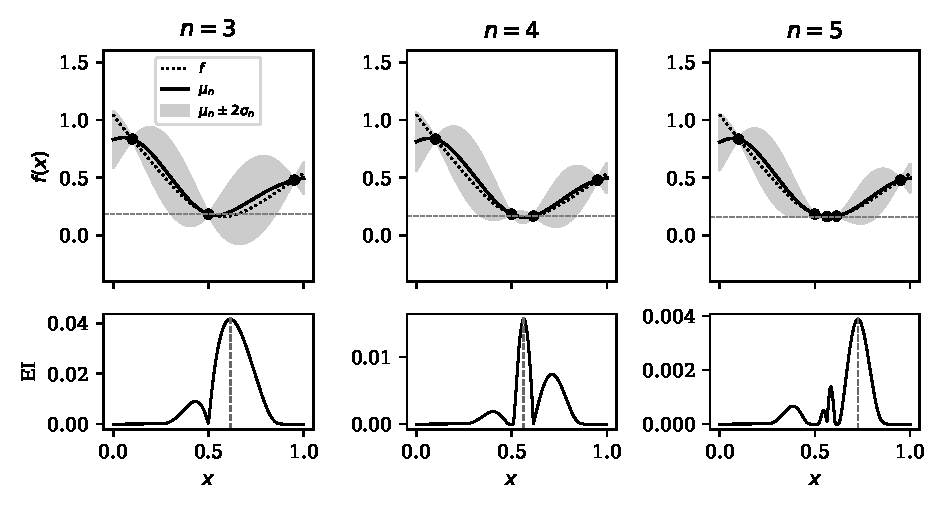
\includegraphics[width=\textwidth]{M25-fig-bo.pdf}
\caption{Tres iteraciones de optimización bayesiana con mejora esperada sobre una función de una variable (Parte~4 de la práctica). Arriba, la función verdadera (punteada), la media posterior y la banda $\pm2\sigma_n$; la línea discontinua horizontal es $\fmejor$. Abajo, la EI y el punto que maximiza (línea vertical). La EI se anula en los puntos ya evaluados y es grande donde la media es baja o la incertidumbre alta.}
\label{fig:bo1d}
\end{figure}

\section{Cotas de confianza y muestreo de Thompson}

\begin{definicion}[Cota inferior de confianza]\label{def:lcb}
Para un parámetro $\beta_n>0$, se elige $x_{n+1}\in\arg\min_x\LCB_n(x)$, con $\LCB_n(x)=\mu_n(x)-\sqrt{\beta_n}\,\sigma_n(x)$. En maximización se usa la cota superior $\UCB_n=\mu_n+\sqrt{\beta_n}\sigma_n$ (GP-UCB).
\end{definicion}

Srinivas \emph{et al.}~\cite{srinivas} demostraron que, con una sucesión $\beta_n$ que crece logarítmicamente, el regret acumulado de GP-UCB crece como $O^*\bigl(\sqrt{N\beta_N\gamma_N}\bigr)$, donde $\gamma_N$ es la máxima información que $N$ observaciones ruidosas pueden aportar sobre $f$; para el núcleo exponencial cuadrático, $\gamma_N$ crece como una potencia de $\log N$, y el regret medio $R_N/N$ tiende a cero. La teoría da una justificación al equilibrio entre explorar y explotar, pero los valores de $\beta_n$ que exige son conservadores; en la práctica se usan constantes entre $1$ y $9$~\cite[§8.4 y cap.~10]{garnett}.

El \emph{muestreo de Thompson} extrae una función $\tilde f\sim\GP(\mu_n,k_n)$ de la posterior y ensaya su mínimo; explora en proporción a la probabilidad de que cada punto sea el óptimo y se paraleliza con facilidad~\cite[§7.9]{garnett}.

\section{Optimizar la función de adquisición}

La función $\alpha_n$ es barata pero multimodal: vale casi cero en la mayor parte del dominio y tiene picos estrechos. Lo habitual es evaluarla en una nube de miles de candidatos (aleatorios y perturbaciones de los mejores puntos) y refinar los mejores con L-BFGS-B, usando su gradiente analítico o por diferenciación automática~\cite[§9.2]{garnett}, \cite{botorch}. Con valores de EI muy pequeños conviene trabajar con su logaritmo para evitar regiones numéricamente planas.

\begin{observacion}[Varianza latente y varianza predictiva]\label{obs:latente}
Muchas bibliotecas devuelven la desviación típica de una nueva \emph{observación}, $\sqrt{\sigma_n^2(x)+\sigma_\varepsilon^2}$, en lugar de la de $f(x)$. Usarla en la EI o en la probabilidad de cumplir una restricción es un error: en un punto ya ensayado la incertidumbre nunca baja del nivel de ruido, la EI no se anula y el algoritmo repite indefinidamente el mismo ajuste. En la práctica, con \texttt{GaussianProcessRegressor} y un \texttt{WhiteKernel}, hay que restar la varianza del ruido. En los experimentos de la práctica con la inyectora, sin esta corrección el algoritmo dedicaba la segunda mitad del presupuesto a repetir ajustes casi idénticos en una esquina del dominio.
\end{observacion}

\section{Restricciones}

\begin{proposicion}[Mejora esperada con restricciones]\label{prop:eic}
Sea el problema de la \cref{def:restricciones} con una restricción $c(x)\le 0$ modelada con un proceso gaussiano independiente del de $f$, con posterior $\N(\mu_c,\sigma_c^2)$, y sea $\fmejor$ el mejor valor \emph{factible}. La mejora restringida $I_c(x)=I(x)\,\mathbf 1[c(x)\le 0]$ tiene esperanza
\[
\EI_c(x)=\EI_n(x)\cdot\Phi\Bigl(\frac{-\mu_c(x)}{\sigma_c(x)}\Bigr).
\]
\end{proposicion}

\begin{proof}
Por la independencia de los dos procesos,\[\E\bigl[I(x)\,\mathbf 1[c(x)\le0]\bigr]=\E[I(x)]\,\Pr[c(x)\le 0],\]y $\Pr[c(x)\le0]=\Phi(-\mu_c/\sigma_c)$ por tipificación.
\end{proof}

Gardner \emph{et al.}~\cite{gardner} y Gelbart, Snoek y Adams~\cite{gelbart} estudian la optimización bayesiana con restricciones desconocidas colocando también un proceso gaussiano sobre cada restricción; el segundo admite además restricciones que se evalúan por separado del objetivo. El producto de la \cref{prop:eic} es la forma más sencilla de combinar ambos modelos~\cite[§11.2]{garnett}. Para una especificación $w(x)\le w_{\max}$, la probabilidad de cumplirla es $\Phi\bigl((w_{\max}-\mu_w)/\sigma_w\bigr)$. Si todavía no hay ningún punto factible, se maximiza solo la probabilidad de factibilidad~\cite[§11.2]{garnett}. Las restricciones conocidas y baratas no se modelan: se imponen al generar los candidatos.

\section{Evaluaciones por lotes}

En una planta se suelen hacer varios ensayos por turno, o hay varias máquinas: se necesita proponer $q$ puntos a la vez. La generalización natural es la \emph{mejora esperada multipunto}~\cite{ginsbourger},
\[
q\text{-}\EI(x^{(1)},\dots,x^{(q)})=\E_n\Bigl[\max\bigl(\fmejor-\min_{j}f(x^{(j)}),0\bigr)\Bigr],
\]
que no tiene forma cerrada útil y se estima por Monte Carlo con la distribución conjunta de los $q$ valores; BoTorch la optimiza con gradientes de Monte Carlo~\cite{botorch}. Dos heurísticas secuenciales más sencillas, de Ginsbourger, Le Riche y Carraro~\cite{ginsbourger}, eligen los puntos uno a uno añadiendo un dato ficticio en cada punto elegido: el \emph{creyente del kriging} usa como valor la media posterior $\mu_n(x^{(j)})$, y el \emph{mentiroso constante} usa un valor fijo $L$ (el mínimo, la media o el máximo observado; cuanto mayor es $L$, más se dispersan los puntos). Como la varianza posterior no depende de los valores (\cref{obs:posterior}), el dato ficticio reduce la incertidumbre alrededor de $x^{(j)}$ y aleja de él al siguiente punto del lote. Si los ensayos terminan en momentos distintos, los pendientes se tratan igual (optimización asíncrona~\cite[§11.4]{garnett}).

\section{Varios objetivos}

En la inyectora se puede querer, en lugar de un único coste, minimizar a la vez la fracción defectuosa y el tiempo de ciclo, y dejar la elección final a la dirección de la planta.

\begin{definicion}[Dominancia y frente de Pareto]\label{def:pareto}
Sean $F(x)=(F_1(x),\dots,F_m(x))$ objetivos a minimizar. El punto $x$ \emph{domina} a $x'$ si $F_i(x)\le F_i(x')$ para todo $i$ y $F_i(x)<F_i(x')$ para algún $i$. Un punto es \emph{óptimo de Pareto} si ningún otro lo domina; la imagen del conjunto de óptimos es el \emph{frente de Pareto}~\cite[§12.1]{kw}, \cite[§9.2]{mn}.
\end{definicion}

\begin{definicion}[Hipervolumen]\label{def:hv}
Dado un punto de referencia $r$ dominado por todos los puntos de interés, el \emph{hipervolumen} de un conjunto $P$ de vectores objetivo es la medida (área en dos dimensiones) de la región $\{v: \exists p\in P,\ p\le v\le r\}$ dominada por $P$ y acotada por $r$.
\end{definicion}

El hipervolumen crece si y solo si se añade un punto no dominado por el conjunto, y por eso es la medida habitual de progreso. La \emph{mejora esperada del hipervolumen} (EHVI) es la generalización de la EI; Daulton, Balandat y Bakshy~\cite{qehvi} la extienden a lotes con restricciones (qEHVI) y la calculan con diferenciación automática. Una alternativa más sencilla es escalarizar.

\begin{proposicion}[Escalarización de Chebyshev]\label{prop:chebyshev}
Sean $w_i>0$ pesos y $z^\star$ un punto ideal con $z^\star_i\le F_i(x)$ para todo $x$. Todo minimizador de $s_w(x)=\max_i w_i\bigl(F_i(x)-z^\star_i\bigr)$ es débilmente óptimo de Pareto: no existe $x'$ con $F_i(x')<F_i(x)$ para todo $i$.
\end{proposicion}

\begin{proof}
Si existiera tal $x'$, entonces $w_i(F_i(x')-z_i^\star)<w_i(F_i(x)-z^\star_i)$ para cada $i$, porque $w_i>0$; tomando el máximo en $i$ en ambos lados (el máximo de cantidades estrictamente menores es estrictamente menor), $s_w(x')<s_w(x)$, contra la minimalidad de $x$.
\end{proof}

ParEGO~\cite{parego} aplica la EI a la escalarización de Chebyshev aumentada con pesos aleatorios distintos en cada iteración, y así recorre el frente. A diferencia de la suma ponderada, la escalarización de Chebyshev alcanza también los puntos de las partes no convexas del frente (\cref{eje:4-chebyshev}).

\section{Varias fidelidades}

A menudo hay versiones más baratas e imprecisas del experimento: una simulación del llenado del molde antes del ensayo en máquina, un ensayo de resistencia a 7 días en lugar de 28, un entrenamiento corto en lugar de uno completo. La optimización multifidelidad modela conjuntamente $f(x,s)$, con $s$ la fidelidad, y elige a la vez el punto y la fidelidad~\cite[§11.5]{garnett}, \cite[§5]{frazier}. La regla más simple es dividir la adquisición por el coste: Snoek, Larochelle y Adams~\cite{snoek} proponen la mejora esperada por segundo, $\EI(x)/c(x)$, con el coste $c(x)$ también modelado. Kandasamy \emph{et al.}~\cite{kandasamy} (MF-GP-UCB) usan las fidelidades baratas para descartar regiones poco prometedoras y reservan las caras para las regiones buenas, con garantías de regret mejores que las de ignorar las aproximaciones.

\section{Caso de estudio: el optimizador de la inyectora}

\begin{ejemplo}[Optimización bayesiana con restricción de alabeo]\label{ej:bo-inyectora}
Se aplica el \cref{alg:bo} al \cref{ej:inyectora} (Parte~4 de la práctica; datos sintéticos). Diseño inicial: LHS de 10 lotes. Sustitutos: dos procesos gaussianos Matérn 5/2 con ARD y ruido estimado, uno para el coste observado y otro para el alabeo medido, ambos con entradas en $[0,1]^3$. Adquisición: EI restringida (\cref{prop:eic}) con la varianza latente (\cref{obs:latente}) y $\fmejor$ igual al mínimo de la media posterior entre los ensayos con probabilidad de cumplir el alabeo de al menos $0{,}5$. Optimización de la adquisición: 4000 candidatos uniformes y 500 perturbaciones gaussianas ($\sigma=0{,}05$) de puntos ya ensayados. Presupuesto: 20 lotes más. Recomendación: el mínimo de la media posterior del coste en $20\,000$ puntos del dominio entre los que tienen $\Pr[w\le0{,}45]\ge0{,}8$. Como referencia se toma la alternativa sin bucle: los 30 lotes en un único LHS y la misma recomendación. Con 10 repeticiones de cada estudio:
\begin{center}\small
\begin{tabular}{@{}lccccc@{}}
\toprule
 & regret & regret & alabeo rec. & lotes fuera & coste medio \\
Método (30 lotes) & mediano (€) & máximo (€) & máximo (mm) & de esp. & lotes (€) \\
\midrule
Optimización bayesiana & $0{,}0066$ & $0{,}0219$ & $0{,}448$ & $39\,\%$ & $0{,}828$ \\
LHS de 30 + PG & $0{,}0170$ & $0{,}0322$ & $0{,}451$ & $68\,\%$ & $0{,}841$ \\
\bottomrule
\end{tabular}
\end{center}
La optimización bayesiana reduce el regret mediano a menos de la mitad, todas sus recomendaciones cumplen la restricción (la del LHS en el peor caso la viola por $0{,}001$~mm), y además produce menos lotes fuera de especificación y más baratos durante el estudio: si los ensayos se hacen en producción, también gana en regret acumulado. Con lotes de dos ensayos por turno ($q=2$, creyente del kriging) el regret mediano es $0{,}0044$~€ en solo 10 rondas: en este problema, paralelizar no cuesta precisión. El regret de $0{,}0066$~€ por pieza supone, frente al óptimo, unos 6600~€ al año por millón de piezas, y el ahorro frente a la receta del operario es de más de $0{,}08$~€ por pieza.
\end{ejemplo}

\begin{table}[ht]
\centering\small
\begin{tabularx}{\textwidth}{@{}>{\raggedright\arraybackslash}p{2.5cm}>{\raggedright\arraybackslash}X>{\raggedright\arraybackslash}p{1.4cm}>{\raggedright\arraybackslash}p{3.8cm}@{}}
\toprule
Herramienta & Para qué sirve & Licencia & Cuándo elegirla \\
\midrule
BoTorch~\cite{botorch} & Adquisiciones de Monte Carlo: qEI, qNEI, qEHVI, multifidelidad, restricciones & MIT & Problemas a medida, lotes, varios objetivos \\
Ax~\cite{ax} & Interfaz de alto nivel sobre BoTorch: experimentos, restricciones de resultado, ensayos pendientes & MIT & Campañas reales con varias personas y máquinas \\
Optuna \texttt{GPSampler}~\cite{optuna} & Optimización bayesiana con PG dentro de Optuna & MIT & Si ya se usa Optuna \\
SMAC3~\cite{smac3} & BO con bosques aleatorios y espacios condicionales & BSD & Variables categóricas y jerárquicas \\
scikit-learn + SciPy & PG y optimización de la adquisición escritos a mano & BSD & Docencia y prototipos (práctica) \\
\bottomrule
\end{tabularx}
\caption{Tecnologías para la optimización bayesiana.}
\label{tab:tec4}
\end{table}

\begin{observacion}[Errores frecuentes en la práctica]\label{obs:errores4}
\begin{enumerate}
  \item Usar la varianza predictiva en lugar de la latente (\cref{obs:latente}).
  \item Tomar como $\fmejor$ el mínimo \emph{observado} con ruido: la maldición del ganador (\cref{prop:ganador}) hace la referencia demasiado optimista y la EI se vuelve tímida.
  \item Optimizar mal la adquisición (pocos candidatos, un único arranque): el algoritmo deja de explorar sin que nadie lo note.
  \item Diseño inicial demasiado pequeño: con 2 o 3 puntos los hiperparámetros son arbitrarios y las primeras decisiones, malas.
  \item Recomendar en la frontera de la restricción sin margen ni confirmación: la mitad de los lotes ensayados exactamente en el límite parecerán violarla (en la práctica, el $49\,\%$ en el óptimo).
  \item Confiar en la BO en dimensión alta (más de unas 20 variables) sin modelos específicos ni regiones de confianza.
\end{enumerate}
\end{observacion}

\begin{lecturas}
\item Jones, Schonlau y Welch~\cite{jones}, §4.1–4.2 (la mejora esperada y el algoritmo EGO).
\item Frazier~\cite{frazier}, §4.1 «Expected Improvement» y §5 «Exotic Bayesian Optimization».
\item Garnett~\cite{garnett}, §7.3, §7.5, §7.8–7.9, §8.2–8.4 y §11.2–11.7.
\item Kochenderfer y Wheeler~\cite{kw}, §16.3–16.6.
\item Shahriari \emph{et al.}~\cite{shahriari}, revisión general.
\end{lecturas}

\section*{Ejercicios del tema 4}
\addcontentsline{toc}{section}{Ejercicios del tema 4}

\begin{ejercicio}{1}{eje:4-pi}
(a) Explique por qué la PI con $\xi=0$ tiende a ensayar puntos pegados al mejor actual. (b) ¿Cuánto vale la EI en un punto ya evaluado si no hay ruido? ¿Y si lo hay y se usa por error la varianza predictiva? (c) ¿Qué representa $\beta_n$ en la LCB y qué ocurre en los límites $\beta_n\to0$ y $\beta_n\to\infty$?
\end{ejercicio}

\begin{ejercicio}{2}{eje:4-calculo}
Con $\fmejor=1{,}00$, calcule PI (con $\xi=0$), EI y $\LCB=\mu-2\sigma$ en los candidatos $P$: $\mu=0{,}98$, $\sigma=0{,}02$; $Q$: $\mu=1{,}05$, $\sigma=0{,}10$; $R$: $\mu=1{,}20$, $\sigma=0{,}30$. ¿Qué punto elige cada criterio? Use $\Phi(1)=0{,}8413$, $\varphi(1)=0{,}2420$, $\Phi(-0{,}5)=0{,}3085$, $\varphi(-0{,}5)=0{,}3521$, $\Phi(-2/3)=0{,}2525$, $\varphi(-2/3)=0{,}3194$.
\fuente{adaptado de Kochenderfer y Wheeler~\cite{kw}, §16.3–16.5 (texto del curso AA222/CS361 de Stanford~\cite{aa222}).}
\end{ejercicio}

\begin{ejercicio}{2}{eje:4-restringida}
En el candidato $A$ del \cref{ej:ei}, el modelo de alabeo da $\mu_w=0{,}44$~mm y $\sigma_w=0{,}02$~mm, con límite $0{,}45$~mm; en $B$, $\mu_w=0{,}40$ y $\sigma_w=0{,}02$. Calcule la EI restringida de ambos (use $\Phi(0{,}5)=0{,}6915$ y $\Phi(2{,}5)=0{,}9938$). ¿Cambia la elección?
\end{ejercicio}

\begin{ejercicio}{2}{eje:4-creyente}
Proceso gaussiano exponencial cuadrático con $\sigma_f=\ell=1$, sin ruido, con una observación en $x=0$. (a) Calcule $\sigma_1^2(0{,}5)$ y $\sigma_1^2(1)$. (b) El primer punto del lote es $x^{(1)}=1$; con el creyente del kriging se añade un dato ficticio en $x=1$. Calcule $\sigma^2(0{,}5)$ y $\sigma^2(1)$ después. (c) Explique por qué el resultado no depende del valor ficticio y por qué el segundo punto del lote ya no se elegirá en $x=1$.
\fuente{adaptado de Ginsbourger, Le Riche y Carraro~\cite{ginsbourger} y de Garnett~\cite{garnett}, §11.3 «Synchronous Batch Observations».}
\end{ejercicio}

\begin{ejercicio}{2}{eje:4-pareto}
Seis ajustes de la inyectora dan (defectos en \%, ciclo en s): $(2{,}0;30)$, $(3{,}0;26)$, $(5{,}0;22)$, $(4{,}0;27)$, $(8{,}0;21)$, $(2{,}5;32)$. (a) Determine el conjunto no dominado. (b) Calcule su hipervolumen respecto a $r=(10;35)$. (c) ¿Cuánto aumentaría el hipervolumen un nuevo punto $(4{,}0;23)$?
\fuente{adaptado de Kochenderfer y Wheeler~\cite{kw}, §12.1 «Pareto Optimality», y de Martins y Ning~\cite{mn}, §9.2.}
\end{ejercicio}

\begin{ejercicio}{2}{eje:4-coste}
Para decidir el siguiente ensayo de la inyectora se puede hacer una simulación de llenado (20~min de cálculo) cuya EI estimada sobre el coste real es $0{,}002$~€, o un lote en máquina (120~min) con EI $0{,}009$~€. (a) Compare la EI por minuto. (b) ¿Qué EI debería tener la simulación para que ambas opciones fueran equivalentes? (c) ¿Qué riesgo tiene este criterio si la simulación está sesgada?
\end{ejercicio}

\begin{ejercicio}{3}{eje:4-ei}
(a) Demuestre que $\EI(\mu,\sigma)\to\max(\fmejor-\mu,0)$ cuando $\sigma\to 0^+$. (b) Demuestre que $\EI$ es convexa en $\mu$ para $\sigma$ fijo. (c) Deduzca la fórmula de la EI cuando se maximiza: $I=\max(f(x)-\fmejor,0)$, y demuestre que puede escribirse como $[\Delta]^++\sigma\varphi(\Delta/\sigma)-\abs{\Delta}\,\Phi(-\abs{\Delta}/\sigma)$ con $\Delta=\mu-\fmejor$, forma usada por Frazier.
\fuente{adaptado de Frazier~\cite{frazier}, §4.1, y de Jones, Schonlau y Welch~\cite{jones}, §4.1.}
\end{ejercicio}

\begin{ejercicio}{3}{eje:4-chebyshev}
Un problema con dos objetivos tiene como conjunto alcanzable los puntos $F^{(1)}=(0;1)$, $F^{(2)}=(1;0)$ y $F^{(3)}=(0{,}6;0{,}6)$. (a) Compruebe que los tres son óptimos de Pareto. (b) Demuestre que ninguna suma ponderada $w_1F_1+w_2F_2$ con $w_i>0$ tiene a $F^{(3)}$ como minimizador. (c) Encuentre pesos de Chebyshev (con $z^\star=(0,0)$) para los que $F^{(3)}$ sea el único minimizador.
\end{ejercicio}

% =====================================================================
\chapter{Casos de estudio: moldeo por inyección y hormigón}
\label{tema:5}
% =====================================================================

Este tema reúne las piezas de los anteriores en dos casos completos: el ajuste de la inyectora, que se ha ido desarrollando desde el \cref{tema:1}, y la formulación de un hormigón con menos emisiones de CO$_2$. Ambos usan datos sintéticos generados por los simuladores de la Parte~5 de la práctica; la revisión de Fernandes \emph{et al.}~\cite{fernandes} sobre modelado y optimización del moldeo por inyección y el trabajo de Ament \emph{et al.}~\cite{ament} sobre hormigón sostenible con optimización bayesiana son las referencias de los procesos reales. La metodología sigue las guías de Montgomery~\cite[§1.5]{montgomery} y Garnett~\cite[cap.~9]{garnett}.

\section{Del problema al optimizador}

\begin{algoritmo}[Lista de diseño de un optimizador experimental]\label{alg:lista}
\begin{enumerate}[label=\arabic*.]
  \item \emph{Objetivo}: una cifra con unidades y su justificación económica (coste por pieza buena, emisiones por m$^3$). Si hay varias, decidir si se escalariza o se busca el frente de Pareto.
  \item \emph{Variables}: las que se pueden fijar en planta, con rangos seguros acordados con quien opera el proceso; escala lineal o logarítmica.
  \item \emph{Restricciones}: clasificarlas (conocidas, caras, ocultas, de seguridad) según el \cref{tema:1}.
  \item \emph{Ruido}: de dónde viene, cuánto vale (réplicas o un estudio previo) y si es heterocedástico.
  \item \emph{Presupuesto y logística}: número de ensayos, cuántos en paralelo, cuánto tarda cada uno y si hay fidelidades más baratas.
  \item \emph{Cribado}: un factorial o una fracción para descartar variables y detectar interacciones.
  \item \emph{Bucle}: diseño inicial, sustituto, adquisición, recomendación (\cref{alg:bo}).
  \item \emph{Parada y confirmación}: criterio de parada (\cref{tema:6}) y ensayos repetidos en la recomendación.
  \item \emph{Registro}: guardar cada ensayo con su contexto (lote de material, turno, operario) para poder reutilizarlo.
\end{enumerate}
\end{algoritmo}

\begin{figure}[ht]
\centering
\begin{tikzpicture}[font=\small,>={Stealth[length=2mm]},
  caja/.style={draw,rounded corners,align=center,minimum height=0.95cm,thick,fill=white},
  dato/.style={draw,align=center,minimum height=0.95cm,dashed}]
  \node[dato] (reg) at (0,0) {registro de\\ensayos};
  \node[caja] (mod) at (3.3,0.9) {sustituto del\\objetivo $\mu_f,\sigma_f$};
  \node[caja] (res) at (3.3,-0.9) {sustitutos de las\\restricciones $\mu_c,\sigma_c$};
  \node[caja] (adq) at (6.9,0) {adquisición\\(EI restringida, lote $q$)};
  \node[caja] (seg) at (10.3,0) {filtro de\\seguridad};
  \node[caja] (ope) at (10.3,-2.2) {aprobación\\del responsable};
  \node[caja] (pla) at (6.9,-2.2) {planta:\\ensayo y medida};
  \draw[->,thick] (reg) -- (mod); \draw[->,thick] (reg) -- (res);
  \draw[->,thick] (mod) -- (adq); \draw[->,thick] (res) -- (adq);
  \draw[->,thick] (adq) -- (seg); \draw[->,thick] (seg) -- (ope);
  \draw[->,thick] (ope) -- (pla); \draw[->,thick] (pla) -| (reg);
\end{tikzpicture}
\caption{Arquitectura de un optimizador experimental en planta. Las restricciones conocidas actúan en el filtro de seguridad, que descarta propuestas fuera de la ventana operativa antes de que lleguen a la persona responsable.}
\label{fig:arquitectura}
\end{figure}

La comparación con la práctica tradicional de variar un factor cada vez (OFAT) muestra por qué se necesita todo lo anterior.

\begin{ejemplo}[Un factor cada vez en un valle oblicuo]\label{ej:ofat}
Sea $f(u_1,u_2)=(u_1-u_2)^2+0{,}05\,(u_1+u_2-2)^2$, con mínimo $f=0$ en $(1,1)$. Partiendo de $(0,0)$, se optimiza primero $u_1$ con $u_2=0$: $\partial f/\partial u_1=2u_1+0{,}1(u_1-2)=0$ da $u_1=0{,}0952$. Después se optimiza $u_2$ con $u_1$ fijo: $-2(u_1-u_2)+0{,}1(u_1+u_2-2)=0$ da $u_2=(1{,}9u_1+0{,}2)/2{,}1=0{,}1814$. Tras una pasada, el experimentador está en $(0{,}095;0{,}181)$ con $f=0{,}156$, lejos del óptimo, y cada nueva pasada avanza poco porque el valle es oblicuo: la interacción $u_1u_2$ (el término cruzado) hace que la mejor elección de una variable dependa de la otra. Un modelo de segundo orden ajustado con un CCD localiza el mínimo con una sola resolución (\cref{prop:estacionario}). Montgomery~\cite[§5.2]{montgomery} da el argumento general de la ventaja de los factoriales sobre OFAT.
\end{ejemplo}

\section{Caso A: el ajuste completo de la inyectora}

\begin{ejemplo}[Inyectora: de la receta del operario al óptimo confirmado]\label{ej:casoA}
Se sigue el \cref{alg:lista} con los datos sintéticos de los temas anteriores.

\emph{1–5. Formulación.} Coste por pieza buena con restricción de alabeo $w\le0{,}45$~mm (\cref{ej:inyectora}); tres variables con rangos seguros; ruido binomial en los defectos (desviación $0{,}0126$~€ en el coste) y de medida en el alabeo ($0{,}009$~mm con 20 piezas); 30 lotes de unas dos horas, dos por turno.

\emph{6. Cribado.} El factorial $2^3$ del \cref{ej:factorial} muestra que el alabeo depende de $T$, de $t_e$ y de su interacción, pero no de $P$ en el rango ensayado. Se mantienen las tres variables porque $P$ controla los defectos, pero se sabe ya que la restricción obligará a alargar el enfriamiento o a bajar la temperatura.

\emph{7. Bucle.} Optimización bayesiana con EI restringida, 10 lotes iniciales y 20 secuenciales (\cref{ej:bo-inyectora}), o 10 rondas de 2 lotes. Mediana de 10 repeticiones: regret $0{,}0066$~€ con lotes de uno y $0{,}0044$~€ con lotes de dos.

\emph{8. Confirmación.} En la repetición de la práctica tomada como ejemplo, el optimizador recomienda $T=200$~°C, $P=84{,}4$~MPa y $t_e=17{,}9$~s, con coste real $0{,}800$~€ y alabeo $0{,}447$~mm. Es un óptimo local en una esquina del dominio, solo dos céntimos peor que el global: la región de bajo coste es una cresta larga a lo largo de la frontera del alabeo, en la que temperatura y presión se compensan (como ya sugería el análisis canónico del \cref{ej:ccd}). Antes de cambiar la receta se ejecutan 5 lotes de confirmación: la media de 5 lotes tiene una desviación de $0{,}0126/\sqrt5=0{,}0056$~€, suficiente para distinguir el nuevo ajuste ($0{,}80$~€) del antiguo ($0{,}87$~€) con holgura. El ahorro confirmado, unos 7 céntimos por pieza, es del $8\,\%$.

\emph{Variante con dos objetivos.} Si la dirección prefiere decidir entre defectos y tiempo de ciclo, los mismos ensayos proporcionan un frente de Pareto: de los 183 lotes que cumplen el alabeo en las 10 repeticiones, 39 son no dominados, con un hipervolumen de $334{,}6$ (unidades \%·s) respecto a la referencia $(20\,\%;\ 45\ \text{s})$. El coste por pieza buena es una escalarización particular de ese frente, con pesos dados por los precios.
\end{ejemplo}

\section{Caso B: un hormigón con menos CO\texorpdfstring{$_2$}{2}}

El cemento es responsable de una fracción importante de las emisiones globales de CO$_2$, lo que motiva sustituir parte de él por adiciones como las cenizas volantes~\cite{ament}. La dificultad es que la resistencia, que se mide rompiendo probetas a los 28 días, baja con la sustitución.

\begin{definicion}[Resistencia característica y resistencia media objetivo]\label{def:fck}
La resistencia característica $f_{ck}$ es el cuantil del $5\,\%$ de la resistencia a compresión a 28 días. Si la resistencia de las amasadas de una mezcla es normal con media $f_{cm}$ y desviación $\sigma_p$ (variabilidad de producción), $f_{ck}=f_{cm}-1{,}645\,\sigma_p$, y para garantizar $f_{ck}$ la mezcla debe tener $f_{cm}\ge f_{ck}+1{,}645\,\sigma_p$.
\end{definicion}

La fórmula es el cuantil de la normal (módulo~0.8, §6.3): $\Pr[f<f_{cm}-1{,}645\sigma_p]=\Phi(-1{,}645)=0{,}05$.

\begin{ejemplo}[Formulación de la mezcla]\label{ej:hormigon}
\emph{Variables.} Relación agua/conglomerante $a/c\in[0{,}35;0{,}60]$, fracción de cemento sustituida por cenizas $s\in[0;0{,}40]$ y contenido de conglomerante $b\in[280;450]$~kg/m$^3$.

\emph{Restricción conocida.} El agua, $(a/c)\,b$, debe estar entre 160 y 195~kg/m$^3$ para que el hormigón sea trabajable. Es barata: se comprueba sin ensayar y se usa para filtrar candidatos.

\emph{Objetivo conocido.} Con factores de emisión de $0{,}93$~kg CO$_2$e por kg de cemento, $0{,}03$ por kg de cenizas y 45~kg/m$^3$ por áridos y transporte (valores de orden de magnitud para el curso), $\gwp(x)=0{,}93\,b(1-s)+0{,}03\,bs+45$~kg~CO$_2$e/m$^3$.

\emph{Restricción cara.} Para un C30 con $\sigma_p=4$~MPa, $f_{28}(x)\ge 30+1{,}645\cdot4=36{,}58$~MPa. Cada ensayo es una amasada con probetas rotas a 7 y 28 días; el ruido de la media de las probetas es de unos 2~MPa. El simulador usa una ley del tipo de Abrams, $f_{28}=105\cdot 8^{-a/c}$~MPa sin cenizas, corregida por la sustitución y por el contenido de conglomerante.

\emph{Partida y óptimo.} La mezcla habitual, $(0{,}50;\ 0;\ 350)$, da $f_{28}=37{,}12$~MPa y $\gwp=370{,}5$. El óptimo del simulador es $(0{,}4225;\ 0{,}225;\ 379)$, con $\gwp=320{,}7$ ($-13{,}4\,\%$) y $f_{28}=36{,}58$ justo en el límite: se baja la relación agua/conglomerante para poder sustituir un $22\,\%$ del cemento, y el agua queda en su mínimo de 160~kg/m$^3$.
\end{ejemplo}

\begin{observacion}[Objetivo conocido, restricción desconocida]\label{obs:objconocido}
Cuando el objetivo $g$ es una fórmula conocida y lo caro es la restricción, la mejora en un candidato es determinista, $I(x)=\max(g^*-g(x),0)$, y la EI restringida de la \cref{prop:eic} se reduce a
\[
\alpha(x)=\max\bigl(g^*-g(x),0\bigr)\cdot\Pr\bigl[f_{28}(x)\ge 36{,}58\bigr]=\max\bigl(g^*-g(x),0\bigr)\cdot\Phi\Bigl(\frac{\mu_{28}(x)-36{,}58}{\sigma_{28}(x)}\Bigr).
\]
Solo hay que modelar lo que no se conoce. La misma idea mejora el caso de la inyectora, cuyo tiempo de ciclo es conocido: basta modelar la fracción defectuosa.
\end{observacion}

\begin{ejemplo}[Programa semanal con optimización bayesiana]\label{ej:casoB}
Se ensayan 6 mezclas iniciales de un LHS filtrado por la restricción de agua y 4 semanas de 3 mezclas, elegidas con la adquisición de la \cref{obs:objconocido} y el creyente del kriging: 18 amasadas en total. La recomendación final minimiza el GWP entre las mezclas con probabilidad posterior de cumplir la resistencia de al menos $0{,}9$. En 6 repeticiones del estudio (Parte~5 de la práctica):
\begin{center}\small
\begin{tabular}{@{}cccccc@{}}
\toprule
Repetición & $a/c$ & $s$ & $b$ (kg/m$^3$) & GWP & $f_{28}$ real (MPa) \\
\midrule
0 & 0{,}451 & 0{,}127 & 357 & 335{,}8 & 37{,}79 \\
1 & 0{,}462 & 0{,}118 & 348 & 331{,}7 & 37{,}12 \\
2 & 0{,}418 & 0{,}202 & 385 & 333{,}2 & 38{,}08 \\
3 & 0{,}469 & 0{,}116 & 343 & 328{,}1 & 36{,}54 \\
4 & 0{,}448 & 0{,}166 & 361 & 327{,}0 & 36{,}80 \\
5 & 0{,}450 & 0{,}132 & 357 & 334{,}8 & 37{,}78 \\
\bottomrule
\end{tabular}
\end{center}
El GWP mediano es $332{,}4$~kg/m$^3$: un $10{,}3\,\%$ menos que la mezcla habitual y $11{,}7$ por encima del óptimo. La distancia al óptimo es el precio de la prudencia: con 18 amasadas y 2~MPa de ruido, el modelo no puede afirmar con probabilidad $0{,}9$ que una mezcla en el límite cumple, y en cinco de las seis repeticiones recomienda mezclas con un margen de 0,2 a 1,5~MPa. En la sexta, la mezcla recomendada queda $0{,}04$~MPa por debajo del objetivo: por eso la recomendación se confirma con amasadas de prueba antes de usarla en obra.

\emph{Baja fidelidad.} La resistencia a 7 días llega tres semanas antes. En los 18 ensayos de una repetición, la correlación entre $f_7$ y $f_{28}$ es $0{,}85$, pero el cociente $f_7/f_{28}$ baja de $0{,}68$ sin cenizas a $0{,}55$ con un $30\,\%$, porque las cenizas reaccionan más despacio. Usar $f_7$ como sustituto directo penalizaría precisamente las mezclas con cenizas; un modelo multifidelidad debe aprender esa dependencia (\cref{eje:5-fidelidad}).
\end{ejemplo}

\begin{ejemplo}[Casos reales publicados]\label{ej:reales}
Ament, Witte, Garg y Kusuma~\cite{ament} formularon el diseño de mezclas de hormigón como un problema con dos objetivos, resistencia a compresión y potencial de calentamiento global, propusieron un modelo de procesos gaussianos para predecir la resistencia a partir de relativamente pocas medidas y ejecutaron optimización bayesiana multiobjetivo con ensayos reales de las mezclas propuestas; según los autores, las mezclas obtenidas consiguen mejores compromisos que las basadas en la práctica industrial, y el código es abierto. En química de síntesis, Shields \emph{et al.}~\cite{shields} compararon la optimización bayesiana con químicos expertos en la optimización de reacciones y encontraron que el algoritmo alcanzaba buenos resultados en menos experimentos de media y con resultados más consistentes.
\end{ejemplo}

\begin{table}[ht]
\centering\small
\begin{tabularx}{\textwidth}{@{}>{\raggedright\arraybackslash}p{2.8cm}>{\raggedright\arraybackslash}X>{\raggedright\arraybackslash}p{2.2cm}>{\raggedright\arraybackslash}p{3.3cm}@{}}
\toprule
Herramienta & Para qué sirve & Licencia o tipo & Cuándo elegirla \\
\midrule
Ax, interfaz \texttt{Client}~\cite{ax} & Pedir ensayos (\texttt{get\_next\_trials}), registrar resultados (\texttt{complete\_trial}), restricciones de resultado, ensayos pendientes & MIT & Campañas en planta o laboratorio con varias personas \\
BoTorch~\cite{botorch} & Adquisiciones con objetivos conocidos, restricciones y multifidelidad & MIT & Formulaciones a medida como la \cref{obs:objconocido} \\
pyDOE3, \texttt{scipy.stats.qmc} & Cribado y diseño inicial & BSD & Fases 6 y 7 de la lista \\
Sustainable\-Concrete~\cite{ament} & Código de los modelos y del bucle de Ament \emph{et al.} & Código abierto (GitHub) & Punto de partida para mezclas reales \\
Hoja de cálculo o base de datos & Registro de ensayos con contexto & — & Siempre: es el activo más valioso \\
\bottomrule
\end{tabularx}
\caption{Tecnologías para desplegar un optimizador experimental.}
\label{tab:tec5}
\end{table}

\begin{observacion}[Errores frecuentes en la práctica]\label{obs:errores5}
\begin{enumerate}
  \item \emph{Optimizar el simulador y no la planta}: un sustituto ajustado a simulaciones hereda sus sesgos; las conclusiones se confirman con ensayos reales.
  \item \emph{Ignorar la deriva}: un lote nuevo de polímero o de cemento cambia la respuesta; se registra como variable de contexto o se reinicia el estudio.
  \item \emph{Recomendaciones sin margen}: un óptimo en la frontera de una restricción de calidad o de seguridad se incumple la mitad de las veces.
  \item \emph{Ensayos imposibles}: proponer mezclas no trabajables o presiones fuera de la máquina por no filtrar las restricciones conocidas.
  \item \emph{Usar la baja fidelidad como si fuera la alta}: el ensayo a 7 días subestima de forma distinta según la composición.
  \item \emph{Perder la trazabilidad}: sin registro del contexto de cada ensayo, los datos no sirven para el siguiente estudio.
\end{enumerate}
\end{observacion}

\begin{lecturas}
\item Montgomery~\cite{montgomery}, §1.5 «Guidelines for Designing Experiments», §5.2 «The Advantage of Factorials» y §11.6 «Mixture Experiments».
\item Fernandes \emph{et al.}~\cite{fernandes}, revisión del modelado y la optimización del moldeo por inyección.
\item Ament \emph{et al.}~\cite{ament}, hormigón sostenible mediante optimización bayesiana.
\item Shields \emph{et al.}~\cite{shields}, optimización bayesiana de reacciones químicas.
\item Garnett~\cite{garnett}, cap.~9 «Implementation» y apéndice~D (bibliografía comentada de aplicaciones).
\end{lecturas}

\section*{Ejercicios del tema 5}
\addcontentsline{toc}{section}{Ejercicios del tema 5}

\begin{ejercicio}{1}{eje:5-lista}
Aplique los puntos 1 a 5 del \cref{alg:lista} a la optimización de una fermentación para producir un aroma: variables temperatura (28–37~°C), pH (5,0–7,0), glucosa inicial (20–80~g/L) e inóculo (1–10~\%); objetivo, título de producto a las 72~h; 4 biorreactores en paralelo; cada tanda dura 4 días.
\end{ejercicio}

\begin{ejercicio}{2}{eje:5-fck}
(a) Calcule la resistencia media objetivo de un C25 con $\sigma_p=3{,}5$~MPa y con $\sigma_p=5$~MPa. (b) Si una planta reduce su variabilidad de 5 a 3,5~MPa, ¿cuántos MPa de margen gana? (c) Con la ley $f_{28}=105\cdot8^{-a/c}$, halle la $a/c$ máxima en cada caso y cuánto puede aumentar gracias a la reducción de la variabilidad.
\end{ejercicio}

\begin{ejercicio}{2}{eje:5-abrams}
Tres amasadas sin cenizas dan $(a/c,\ f_{28})=(0{,}40;\ 45{,}7)$, $(0{,}50;\ 37{,}1)$ y $(0{,}60;\ 30{,}2)$ (MPa). (a) Ajuste la ley de Abrams $f=A/B^{a/c}$ por mínimos cuadrados sobre $\log f$. (b) Halle la $a/c$ máxima que garantiza $36{,}58$~MPa. (c) ¿Por qué conviene ajustar en escala logarítmica?
\end{ejercicio}

\begin{ejercicio}{2}{eje:5-adquisicion}
Con $g^*=335$~kg~CO$_2$e/m$^3$, tres candidatos tienen $(\gwp,\ \Pr[f_{28}\ge36{,}58])$: $X_1=(325;\ 0{,}70)$, $X_2=(300;\ 0{,}10)$, $X_3=(340;\ 0{,}99)$. Calcule la adquisición de la \cref{obs:objconocido} y ordene los candidatos. Calcule también el GWP, el agua y el coste (cemento $0{,}13$~€/kg, cenizas $0{,}05$~€/kg, 55~€/m$^3$ fijos) de la mezcla $(0{,}45;\ 0{,}15;\ 360)$.
\end{ejercicio}

\begin{ejercicio}{2}{eje:5-mezclas}
Un conglomerante se forma con cemento, cenizas y escoria en fracciones $x_1+x_2+x_3=1$, $x_i\ge0$. (a) Describa la región como un símplice y dibújela. (b) Liste los puntos del diseño de retícula $\{3,2\}$ (fracciones $0$, $\tfrac12$, $1$). (c) Si además $x_1\ge0{,}5$, ¿qué puntos quedan y cuál es la nueva región?
\fuente{adaptado de Montgomery~\cite{montgomery}, §11.6 «Mixture Experiments», y de STAT~503~\cite{psu503}, lección~11.}
\end{ejercicio}

\begin{ejercicio}{2}{eje:5-fidelidad}
Una amasada con $s=0{,}20$ da $f_7=22{,}0$~MPa. (a) Con el cociente $f_7/f_{28}=0{,}68-0{,}45s$, estime $f_{28}$. (b) Si el cociente tiene una incertidumbre de $\pm0{,}03$ (una desviación típica), propague la incertidumbre a $f_{28}$ con la aproximación lineal. (c) ¿Se puede decidir ya que la mezcla cumple $36{,}58$~MPa con probabilidad $0{,}9$?
\end{ejercicio}

\begin{ejercicio}{3}{eje:5-ofat}
(a) Demuestre que si $f(u)=\sum_jf_j(u_j)$ (sin interacciones), una sola pasada de un factor cada vez con minimización exacta en cada variable encuentra el mínimo global. (b) Para $f(u_1,u_2)=(u_1-u_2)^2+0{,}05(u_1+u_2-2)^2$, reproduzca la pasada del \cref{ej:ofat} y calcule el punto tras una segunda pasada. (c) Relacione el resultado con el número de condición de la hessiana y con el descenso por coordenadas del módulo~7.
\fuente{adaptado de Montgomery~\cite{montgomery}, §5.2 «The Advantage of Factorials».}
\end{ejercicio}

\begin{ejercicio}{3}{eje:5-fermentacion}
Diseño razonado. Para la fermentación del \cref{eje:5-lista}, con un presupuesto de 40 tandas (10 semanas) y la posibilidad de medir el título a las 24~h como baja fidelidad, diseñe el optimizador completo: cribado, diseño inicial, sustitutos, adquisición por lotes de 4, uso de la baja fidelidad, regla de parada y confirmación. Justifique cada elección con resultados de los temas~2 a~4 y estime cuántas tandas dedica a cada fase.
\end{ejercicio}

% =====================================================================
\chapter{Ajuste de hiperparámetros, validación y parada}
\label{tema:6}
% =====================================================================

Elegir la tasa de aprendizaje, la regularización o la arquitectura de un modelo es un problema de caja negra con las mismas características que el ajuste de una inyectora: cada evaluación es un entrenamiento caro, el resultado es ruidoso (depende de la semilla y de la partición de los datos) y el presupuesto es limitado. Tiene además dos rasgos propios: espacios mixtos y condicionales, y evaluaciones parciales baratas (pocas épocas, un subconjunto de los datos). Este tema sigue el capítulo~1 del libro de AutoML de Hutter, Kotthoff y Vanschoren, escrito por Feurer y Hutter~\cite{feurer}, y los artículos originales de la búsqueda aleatoria~\cite{bergstra12}, TPE~\cite{tpe}, Hyperband~\cite{hyperband} y ASHA~\cite{asha}. Cierra el módulo con dos preguntas comunes a todos los casos: cómo validar el sustituto y cuándo dejar de experimentar.

\section{El ajuste de hiperparámetros como optimización de caja negra}

\begin{definicion}[Problema de ajuste de hiperparámetros]\label{def:hpo}
Sea $\mathcal A_\lambda$ un algoritmo de aprendizaje con configuración $\lambda\in\Lambda$, entrenado con $D_{\mathrm{ent}}$. El problema es\[\min_{\lambda\in\Lambda}\ \mathcal L\bigl(\mathcal A_\lambda(D_{\mathrm{ent}}),D_{\mathrm{val}}\bigr),\]donde $\mathcal L$ es la pérdida de validación (o la media de una validación cruzada, módulo~8, §6.5). El espacio $\Lambda$ puede mezclar variables continuas, enteras y categóricas, y tener variables \emph{condicionales} (el momento solo existe si el optimizador es SGD)~\cite[§1.2]{feurer}.
\end{definicion}

Las variables que abarcan varios órdenes de magnitud (tasa de aprendizaje, regularización) se buscan en escala logarítmica. Las evaluaciones parciales (un entrenamiento de $r$ épocas en lugar de $R$) son fidelidades bajas, y su aprovechamiento es el origen de los métodos de la §\ref{sec:hyperband}~\cite[§1.4]{feurer}. Las leyes de escalado del módulo~16 son la versión extrema de esta idea para los LLM: se ajustan hiperparámetros y curvas en modelos pequeños y se extrapolan.

\begin{ejemplo}[Dos casos públicos]\label{ej:alphago}
Chen \emph{et al.}~\cite{alphago} describen el uso de optimización bayesiana para ajustar los hiperparámetros de AlphaGo durante su desarrollo. Antes de la partida contra Lee Sedol, el ajuste elevó la tasa de victorias en autojuego de la versión más reciente del 50\,\% al 66,5\,\%, y esa versión ajustada fue la que jugó la partida final. Golovin \emph{et al.}~\cite{vizier} describen Google Vizier, el servicio interno de optimización de caja negra que se convirtió en la herramienta principal de Google para el ajuste de parámetros, usada en muchos modelos y como base del ajuste de hiperparámetros de su servicio de aprendizaje automático en la nube.
\end{ejemplo}

\section{Búsqueda aleatoria frente a rejilla}

\begin{proposicion}[Garantía de la búsqueda aleatoria]\label{prop:aleatoria}
Sea $\Lambda_q\subset\Lambda$ la región de las configuraciones del mejor $q$ (en probabilidad bajo la distribución de muestreo). Con $n$ configuraciones independientes, $\Pr[\text{alguna cae en }\Lambda_q]=1-(1-q)^n$. En consecuencia, para garantizarlo con probabilidad $p$ basta
\[
n\ge\frac{\log(1-p)}{\log(1-q)} .
\]
\end{proposicion}

\begin{proof}
Cada configuración cae fuera de $\Lambda_q$ con probabilidad $1-q$; por independencia, todas caen fuera con probabilidad $(1-q)^n$. La condición $1-(1-q)^n\ge p$ equivale a $n\log(1-q)\le\log(1-p)$, y al dividir por $\log(1-q)<0$ se invierte la desigualdad.
\end{proof}

Con $q=0{,}05$ y $p=0{,}95$ salen $n\ge 58{,}4$: 59 ensayos, independientemente de la dimensión. La garantía es sobre cuantiles del espacio, no sobre la distancia al óptimo, pero explica por qué la búsqueda aleatoria es una línea base difícil de batir. Bergstra y Bengio~\cite{bergstra12} añaden el argumento de la \emph{dimensión efectiva baja}: en la mayoría de los problemas solo unos pocos hiperparámetros importan, y cuáles importan cambia de un conjunto de datos a otro. Una rejilla de $n=m^d$ puntos solo prueba $m=n^{1/d}$ valores de cada hiperparámetro; $n$ puntos aleatorios prueban $n$ valores distintos de cada uno (la misma propiedad de proyección del hipercubo latino, \cref{tema:2}).

\section{El estimador de Parzen con estructura de árbol (TPE)}

La optimización bayesiana con procesos gaussianos modela $p(y\mid\lambda)$. TPE modela al revés: la distribución de las configuraciones condicionada a que sean buenas o malas~\cite[§4]{tpe}.

\begin{definicion}[TPE]\label{def:tpe}
Sea $y^*$ el cuantil $\gamma$ de las pérdidas observadas, de modo que $\Pr[y<y^*]=\gamma$. Se definen dos densidades sobre $\Lambda$, estimadas con núcleos (estimadores de Parzen) a partir de las configuraciones observadas:
\[
p(\lambda\mid y)=\begin{cases}\ell(\lambda)&\text{si } y<y^*\ \text{(configuraciones buenas)},\\ g(\lambda)&\text{si } y\ge y^*\ \text{(el resto)}.\end{cases}
\]
En espacios condicionales, cada hiperparámetro tiene su propia densidad unidimensional y la estructura de árbol decide cuáles intervienen.
\end{definicion}

\begin{proposicion}[TPE maximiza la mejora esperada]\label{prop:tpe}
Con la mejora respecto a $y^*$, $\EI_{y^*}(\lambda)=\int_{-\infty}^{y^*}(y^*-y)\,p(y\mid\lambda)\,dy$, el modelo de la \cref{def:tpe} da
\[
\EI_{y^*}(\lambda)\ \propto\ \Bigl(\gamma+\frac{g(\lambda)}{\ell(\lambda)}(1-\gamma)\Bigr)^{-1},
\]
con una constante de proporcionalidad que no depende de $\lambda$. Maximizar la EI equivale a maximizar el cociente $\ell(\lambda)/g(\lambda)$.
\end{proposicion}

\begin{proof}
Por la regla de Bayes, $p(y\mid\lambda)=p(\lambda\mid y)p(y)/p(\lambda)$. Para $y<y^*$, $p(\lambda\mid y)=\ell(\lambda)$ no depende de $y$, luego
\[
\EI_{y^*}(\lambda)=\frac{\ell(\lambda)}{p(\lambda)}\int_{-\infty}^{y^*}(y^*-y)p(y)\,dy=\frac{\ell(\lambda)\,c}{p(\lambda)},\qquad c=\gamma y^*-\int_{-\infty}^{y^*}y\,p(y)\,dy,
\]
y $c$ no depende de $\lambda$. Por la probabilidad total, $p(\lambda)=\gamma\ell(\lambda)+(1-\gamma)g(\lambda)$. Dividiendo numerador y denominador por $\ell(\lambda)$ se obtiene $\EI_{y^*}(\lambda)=c\,\bigl(\gamma+(1-\gamma)g(\lambda)/\ell(\lambda)\bigr)^{-1}$, que es creciente en $\ell/g$.
\end{proof}

En la práctica TPE muestrea muchos candidatos de $\ell$ y se queda con el de mayor cociente $\ell/g$. Su coste es lineal en el número de observaciones, maneja con naturalidad variables categóricas y condicionales, y es el muestreador por defecto de Optuna~\cite{optuna}. Bergstra \emph{et al.}~\cite[§6]{tpe} usan $\gamma=0{,}15$ en sus experimentos.

\section{Evaluaciones parciales: Successive Halving y Hyperband}
\label{sec:hyperband}

\begin{definicion}[Successive Halving]\label{def:sh}
Dados $n$ configuraciones, un recurso mínimo $r$ (épocas, iteraciones, fracción de datos) y un factor $\eta>1$ (habitualmente 3): se entrenan todas con $r$, se conserva la mejor fracción $1/\eta$, se multiplica el recurso por $\eta$ y se repite hasta que queda una configuración o se alcanza el recurso máximo $R$.
\end{definicion}

El método supone que las configuraciones malas se reconocen pronto. Si se fija el presupuesto total, hay que elegir entre muchas configuraciones con poco recurso (riesgo de descartar las que empiezan despacio) o pocas con mucho (poca exploración). Hyperband no elige: ejecuta varias versiones~\cite[§3.2]{hyperband}.

\begin{algoritmo}[Hyperband]\label{alg:hyperband}
Datos: recurso máximo $R$ y $\eta$. Sean $s_{\max}=\lfloor\log_\eta R\rfloor$ y $B=(s_{\max}+1)R$. Para $s=s_{\max},s_{\max}-1,\dots,0$ (cada valor es un \emph{bracket}):
\begin{enumerate}[label=\arabic*.]
  \item $n=\bigl\lceil\frac{B}{R}\frac{\eta^{s}}{s+1}\bigr\rceil$ configuraciones aleatorias y recurso inicial $r=R\eta^{-s}$;
  \item Successive Halving en $s+1$ rondas: en la ronda $i=0,\dots,s$, $n_i=\lfloor n\eta^{-i}\rfloor$ configuraciones con recurso $r_i=r\eta^{i}$; se conservan las $\lfloor n_i/\eta\rfloor$ mejores.
\end{enumerate}
Se devuelve la mejor configuración evaluada con el recurso completo.
\end{algoritmo}

\begin{proposicion}[Presupuesto de un bracket]\label{prop:bracket}
En el bracket $s$, cada ronda consume como mucho $nr\le\frac{B}{s+1}+R\eta^{-s}$ unidades de recurso, y el bracket completo, como mucho $B+(s+1)R\eta^{-s}$. Todos los brackets cuestan, pues, aproximadamente $B$, y un ciclo de Hyperband, unas $(s_{\max}+1)B$.
\end{proposicion}

\begin{proof}
En la ronda $i$, $n_ir_i\le n\eta^{-i}\cdot r\eta^{i}=nr$. Como $n<\frac{B}{R}\frac{\eta^{s}}{s+1}+1$ y $r=R\eta^{-s}$, se tiene $nr<\frac{B}{s+1}+R\eta^{-s}$. Sumando las $s+1$ rondas se obtiene la segunda cota.
\end{proof}

\begin{ejemplo}[Brackets con $R=81$ y $\eta=3$]\label{ej:brackets}
Se tiene $s_{\max}=4$ y $B=405$. Aplicando el \cref{alg:hyperband} se obtienen, como pares $(n_i,r_i)$:
\begin{center}\small
\begin{tabular}{@{}cll r@{}}
\toprule
$s$ & rondas & & recurso \\
\midrule
4 & $(81,1)\ (27,3)\ (9,9)\ (3,27)\ (1,81)$ & & 405 \\
3 & $(34,3)\ (11,9)\ (3,27)\ (1,81)$ & & 363 \\
2 & $(15,9)\ (5,27)\ (1,81)$ & & 351 \\
1 & $(8,27)\ (2,81)$ & & 378 \\
0 & $(5,81)$ & & 405 \\
\bottomrule
\end{tabular}
\end{center}
El ciclo completo evalúa 143 configuraciones con 1902 unidades de recurso, el equivalente a 23,5 entrenamientos completos. El bracket $s=4$ es el más agresivo (81 configuraciones, casi todas con una sola iteración); el $s=0$ es una búsqueda aleatoria clásica con 5 configuraciones completas, que protege frente a los casos en que las evaluaciones cortas engañan.
\end{ejemplo}

Hyperband es síncrono: cada ronda espera a que terminen todas sus configuraciones. ASHA~\cite{asha} lo hace asíncrono: un trabajador libre promueve a la siguiente ronda cualquier configuración que esté entre la mejor fracción $1/\eta$ de las ya completadas en la suya, o empieza una nueva; así escala linealmente con cientos de trabajadores. Optuna implementa ambos como \emph{pruners}, y BOHB combina Hyperband con un modelo tipo TPE para elegir las configuraciones~\cite[§1.4.2]{feurer}.

\section{Validación del sustituto}

Antes de confiar en las recomendaciones de un sustituto conviene comprobar que predice bien y que sus intervalos están calibrados. Para un proceso gaussiano, la validación cruzada dejando uno fuera no exige reajustar el modelo.

\begin{teorema}[Validación cruzada exacta de un proceso gaussiano]\label{teo:loo}
Con hiperparámetros fijos, la distribución predictiva de la observación $y_i$ dados los demás datos es normal con
\[
\mu_{-i}=y_i-\frac{[\Ky^{-1}y]_i}{[\Ky^{-1}]_{ii}},\qquad \sigma_{-i}^2=\frac{1}{[\Ky^{-1}]_{ii}} .
\]
\end{teorema}

\begin{proof}
Se reordena para que $i$ sea el último índice y se escribe $\Ky=\bigl(\begin{smallmatrix}A&b\\b^\top&c\end{smallmatrix}\bigr)$, con $A$ la matriz de los demás puntos. Por el \cref{lem:condicion} aplicado a $y\sim\N(0,\Ky)$, $y_i\mid y_{-i}\sim\N\bigl(b^\top A^{-1}y_{-i},\ c-b^\top A^{-1}b\bigr)$. Por la fórmula de la inversa por bloques, el último elemento diagonal de $\Ky^{-1}$ es $1/(c-b^\top A^{-1}b)$ (el inverso del complemento de Schur), lo que da $\sigma_{-i}^2$; y la última fila de $\Ky^{-1}$ es $\sigma_{-i}^{-2}\,(-b^\top A^{-1},\ 1)$, luego $[\Ky^{-1}y]_i=\sigma_{-i}^{-2}(y_i-b^\top A^{-1}y_{-i})$. Despejando, $b^\top A^{-1}y_{-i}=y_i-\sigma_{-i}^2[\Ky^{-1}y]_i$, que es $\mu_{-i}$.
\end{proof}

Rasmussen y Williams~\cite[cap.~5]{rw} dan el mismo resultado y lo usan como alternativa a la verosimilitud marginal para elegir hiperparámetros. Con las predicciones LOO se calculan los \emph{residuos tipificados} $r_i=(y_i-\mu_{-i})/\sigma_{-i}$: si el modelo es correcto, se comportan aproximadamente como normales estándar, con media próxima a 0, desviación próxima a 1 y un $5\,\%$ fuera de $\pm2$. Una desviación mucho mayor que 1 revela un modelo demasiado confiado (intervalos estrechos); mucho menor, uno demasiado cauto.

\begin{ejemplo}[Validación del sustituto del coste]\label{ej:loo}
Para el proceso gaussiano del coste al final de una ejecución del \cref{ej:bo-inyectora} (30 lotes), los residuos tipificados LOO tienen media $0{,}01$ y desviación $1{,}05$, y un $7\,\%$ cae fuera de $\pm2$ (2 de 30). El modelo está razonablemente calibrado; las fórmulas cerradas coinciden con el reajuste explícito sin cada punto (Parte~6 de la práctica).
\end{ejemplo}

\section{Cuándo dejar de experimentar}

No existe una regla universal; Garnett~\cite[§5.4 y §9.3]{garnett} trata la parada como una decisión más, que compara el valor esperado de seguir con su coste. Las reglas habituales son:
\begin{enumerate}
  \item \emph{Presupuesto agotado}: la más común y la única que garantiza el plazo.
  \item \emph{Mejora esperada pequeña}: Jones, Schonlau y Welch~\cite[§4.2]{jones} detienen EGO cuando la máxima EI es menor que el $1\,\%$ del mejor valor actual. Con ruido es engañosa: en el caso de la inyectora se activa en el ensayo 13 de 30, cuando la recomendación aún puede mejorar mucho, porque la EI calculada con la varianza latente es pequeña en todas partes salvo en regiones que la adquisición todavía no ha encontrado.
  \item \emph{Cota de regret}: si las bandas de confianza son válidas, la distancia al óptimo de la recomendación está acotada (\cref{prop:cota}). Makarova \emph{et al.}~\cite{makarova} proponen parar cuando esta cota es menor que el error estadístico con que se estima la propia pérdida de validación: seguir optimizando sería ajustar el ruido.
  \item \emph{Criterio económico}: parar cuando la mejora esperada por unidad de producto multiplicada por el volumen de producción sea menor que el coste de un ensayo más.
\end{enumerate}

\begin{proposicion}[Cota del regret simple]\label{prop:cota}
Si con probabilidad al menos $1-\delta$ se cumple $\LCB_n(x)\le f(x)\le\UCB_n(x)$ para todo $x\in\X$, entonces, con la misma probabilidad, para cualquier recomendación $\hat x$,
\[
f(\hat x)-\min_{x\in\X}f(x)\le\UCB_n(\hat x)-\min_{x\in\X}\LCB_n(x).
\]
\end{proposicion}

\begin{proof}
En el suceso en que las bandas son válidas, $f(\hat x)\le\UCB_n(\hat x)$ y, para el minimizador $x^\star$, $f(x^\star)\ge\LCB_n(x^\star)\ge\min_x\LCB_n(x)$. Restando se obtiene la cota.
\end{proof}

La cota es pequeña cuando el modelo está seguro del valor en la recomendación y ningún otro punto tiene una cota inferior mucho más baja: es decir, cuando ya no queda ninguna región sin explorar que pudiera esconder algo mejor.

\section{Caso de estudio: ajuste de un \emph{gradient boosting}}

\begin{ejemplo}[Búsqueda aleatoria, TPE y Hyperband]\label{ej:hpo}
Se ajusta un modelo de \emph{gradient boosting} (\texttt{HistGradient\-Boosting\-Regressor} de scikit-learn) sobre el problema sintético de Friedman (diez variables, cinco relevantes, ruido gaussiano de desviación~1, de modo que el error mínimo alcanzable es $\mathrm{RMSE}=1$), con 600 ejemplos de entrenamiento, 400 de validación y 2000 de prueba (Parte~6 de la práctica). Cuatro hiperparámetros: tasa de aprendizaje en $[0{,}01;0{,}5]$ (logarítmica), número máximo de hojas en $\{4,\dots,64\}$, mínimo de muestras por hoja en $\{2,\dots,60\}$ y regularización $L^2$ en $[10^{-4};10]$ (logarítmica). El recurso es el número de iteraciones de \emph{boosting}, con $R=81$. Media de 3 semillas:
\begin{center}\small
\begin{tabular}{@{}lccc@{}}
\toprule
Método & RMSE val. & RMSE prueba & Iteraciones \\
\midrule
Búsqueda aleatoria (27 configuraciones) & $1{,}451$ & $1{,}528$ & 2187 \\
TPE, Optuna (27 configuraciones) & $1{,}427$ & $1{,}483$ & 2187 \\
Hyperband (un ciclo, 143 configuraciones) & $1{,}456$ & $1{,}517$ & 1902 \\
\bottomrule
\end{tabular}
\end{center}
Tres conclusiones. (i) TPE obtiene el mejor resultado con el mismo presupuesto que la búsqueda aleatoria, gracias a que concentra las últimas 19 configuraciones en la región buena. (ii) Hyperband iguala a la búsqueda aleatoria con un $13\,\%$ menos de cómputo; su ventaja crece cuando el recurso máximo es mucho mayor que el necesario para distinguir configuraciones, como al entrenar redes durante muchas épocas. (iii) En los tres casos el error de prueba supera al de validación en 0,05–0,08: es la maldición del ganador (\cref{prop:ganador}) aplicada a la selección de hiperparámetros. El error de validación de la configuración elegida es una estimación optimista; para informar del rendimiento se necesita un conjunto de prueba que no haya intervenido en la selección (validación anidada). Con tres semillas, las diferencias entre métodos son del orden de su variabilidad: una comparación seria exige más repeticiones.
\end{ejemplo}

\begin{table}[ht]
\centering\small
\begin{tabularx}{\textwidth}{@{}>{\raggedright\arraybackslash}p{2.8cm}>{\raggedright\arraybackslash}X>{\raggedright\arraybackslash}p{1.4cm}>{\raggedright\arraybackslash}p{3.5cm}@{}}
\toprule
Herramienta & Para qué sirve & Licencia & Cuándo elegirla \\
\midrule
Optuna~\cite{optuna} & TPE, GP, CMA-ES, NSGA-II; \emph{pruners} \texttt{SuccessiveHalvingPruner}, \texttt{HyperbandPruner}, \texttt{MedianPruner} & MIT & Opción por defecto en Python, espacios definidos al ejecutar \\
SMAC3~\cite{smac3} & BO con bosques aleatorios, Hyperband, configuración sobre varias instancias & BSD & Espacios condicionales, configuración de algoritmos \\
Ax y BoTorch~\cite{ax,botorch} & BO con GP, multiobjetivo y parada temprana & MIT & Pocos ensayos muy caros, varios objetivos \\
scikit-learn & \texttt{RandomizedSearchCV} y búsqueda por reducción sucesiva & BSD & Modelos de scikit-learn con validación cruzada \\
Google Vizier~\cite{vizier} & Servicio de optimización de caja negra con parada temprana y transferencia & Servicio & Referencia de diseño de un servicio a escala \\
\bottomrule
\end{tabularx}
\caption{Tecnologías para el ajuste de hiperparámetros.}
\label{tab:tec6}
\end{table}

\begin{observacion}[Errores frecuentes en la práctica]\label{obs:errores6}
\begin{enumerate}
  \item \emph{Fuga de datos}: ajustar hiperparámetros con el conjunto de prueba, o preprocesar (normalizar, seleccionar variables) con todos los datos antes de dividirlos.
  \item \emph{Informar del error de validación del ganador}: es optimista; se usa un conjunto de prueba aparte o validación anidada.
  \item \emph{Una sola semilla}: con entrenamientos ruidosos, la diferencia entre dos configuraciones puede ser solo la semilla.
  \item \emph{Rangos lineales} para tasas de aprendizaje o regularizaciones.
  \item \emph{Poda demasiado agresiva}: Successive Halving descarta configuraciones que empiezan despacio (tasas de aprendizaje pequeñas); por eso Hyperband conserva brackets conservadores.
  \item \emph{Ignorar el coste}: comparar métodos por número de configuraciones y no por cómputo total.
\end{enumerate}
\end{observacion}

\begin{lecturas}
\item Feurer y Hutter~\cite{feurer}, §1.2–1.4 (problema, métodos de caja negra y multifidelidad).
\item Bergstra y Bengio~\cite{bergstra12}, búsqueda aleatoria y dimensión efectiva.
\item Bergstra \emph{et al.}~\cite{tpe}, §4 «Tree-structured Parzen Estimator Approach».
\item Li \emph{et al.}~\cite{hyperband}, §3.1–3.2 (Successive Halving y Hyperband) y Li \emph{et al.}~\cite{asha} (ASHA).
\item Garnett~\cite{garnett}, §5.4 y §9.3 (parada como decisión); Makarova \emph{et al.}~\cite{makarova}.
\end{lecturas}

\section*{Ejercicios del tema 6}
\addcontentsline{toc}{section}{Ejercicios del tema 6}

\begin{ejercicio}{1}{eje:6-rejilla}
Con 9 ensayos para dos hiperparámetros de los que solo uno influye, compare cuántos valores distintos del hiperparámetro relevante prueban una rejilla $3\times3$ y una búsqueda aleatoria. ¿Y con 64 ensayos en 3 hiperparámetros?
\fuente{adaptado de Bergstra y Bengio~\cite{bergstra12} (argumento de la dimensión efectiva).}
\end{ejercicio}

\begin{ejercicio}{2}{eje:6-aleatoria}
Con la \cref{prop:aleatoria}: (a) ¿cuántos ensayos garantizan con probabilidad $0{,}95$ caer en el mejor $2\,\%$? (b) ¿Y con probabilidad $0{,}99$ en el mejor $5\,\%$? (c) Con 27 ensayos, ¿qué probabilidad hay de caer en el mejor $5\,\%$?
\fuente{adaptado de Feurer y Hutter~\cite{feurer}, §1.3.1 «Model-Free Blackbox Optimization Methods».}
\end{ejercicio}

\begin{ejercicio}{2}{eje:6-hyperband}
Aplique el \cref{alg:hyperband} con $R=27$ y $\eta=3$: calcule $s_{\max}$, $B$, los brackets con sus pares $(n_i,r_i)$ y el recurso total. ¿A cuántos entrenamientos completos equivale?
\fuente{adaptado de Li \emph{et al.}~\cite{hyperband}, §3.2, algoritmo~1.}
\end{ejercicio}

\begin{ejercicio}{2}{eje:6-tpe}
Con $\gamma=0{,}15$, tres candidatos tienen densidades $(\ell,g)$: $\lambda_1=(2{,}0;\ 0{,}5)$, $\lambda_2=(1{,}0;\ 1{,}0)$ y $\lambda_3=(0{,}4;\ 0{,}05)$. Calcule la cantidad proporcional a la EI de la \cref{prop:tpe} y ordénelos. Comente por qué el candidato con mayor $\ell$ no es el elegido.
\end{ejercicio}

\begin{ejercicio}{3}{eje:6-tpeprueba}
(a) Complete los detalles de la demostración de la \cref{prop:tpe}, justificando que $c>0$. (b) Demuestre que la proporcionalidad se conserva si $y^*$ es el cuantil $\gamma$ de una distribución continua cualquiera de $y$. (c) ¿Qué ocurre en el límite $\gamma\to 0$?
\fuente{adaptado de Bergstra \emph{et al.}~\cite{tpe}, §4.1.}
\end{ejercicio}

\begin{ejercicio}{2}{eje:6-loo}
Con los datos del \cref{ej:gp2} y ruido $\sigma_n=0{,}1$, calcule $\Ky^{-1}$ y, con el \cref{teo:loo}, la media y la varianza LOO de $y_1$ y de $y_2$. Compruebe el resultado de $y_1$ condicionando directamente con el \cref{lem:condicion}.
\end{ejercicio}

\begin{ejercicio}{2}{eje:6-parada}
En una iteración de la inyectora, la máxima EI restringida es $0{,}004$~€, el mejor coste predicho es $0{,}785$~€, $\UCB(\hat x)=0{,}795$~€ y $\min_x\LCB(x)=0{,}770$~€. (a) ¿Para la regla de Jones \emph{et al.}? (b) ¿Qué cota da la \cref{prop:cota}? (c) Con una producción de $10^6$ piezas al año y 300~€ por ensayo, ¿compensa seguir según el criterio económico? (d) ¿Qué conclusión sacaría si la desviación del coste medido en un lote es $0{,}0126$~€?
\end{ejercicio}

\begin{ejercicio}{1}{eje:6-fuga}
Un equipo prueba 200 configuraciones y publica el error de validación de la mejor como rendimiento esperado del modelo. Explique, con la \cref{prop:ganador}, por qué es optimista y describa un procedimiento de validación anidada que lo evite.
\end{ejercicio}

\begin{ejercicio}{3}{eje:6-llm}
Diseño razonado. Hay que ajustar un modelo de lenguaje de 1000 millones de parámetros con LoRA para una tarea de clasificación de incidencias de planta. Hiperparámetros: tasa de aprendizaje, rango de LoRA ($\{4,8,16,32,64\}$), número de épocas (1–5), proporción de calentamiento y \emph{dropout}. Presupuesto: 200 horas de GPU; un entrenamiento completo dura 4 horas. Diseñe la estrategia: espacio de búsqueda y escalas, método (justificando entre búsqueda aleatoria, TPE, Hyperband/ASHA y BO), recurso para las fidelidades bajas, número de semillas, validación y criterio de parada.
\end{ejercicio}


\appendix
% =====================================================================
\chapter{Soluciones de los ejercicios}
\label{ap:soluciones}
% =====================================================================

Cada solución se presenta en cinco partes: datos, planteamiento, desarrollo, resultado y comprobación. En los pasos intermedios se redondea a cuatro cifras significativas salvo que se indique otra cosa. Los ejercicios de diseño razonado no tienen una única respuesta correcta; la solución propone una y justifica cada decisión.

% ---------------------------------------------------------------------
\section{Tema 1}

\begin{solucion}{eje:1-clasificar}
\datos cuatro situaciones.
\planteamiento aplicar la \cref{def:cajanegra} y la \cref{def:regret}: ¿se conoce $f$ como fórmula?, ¿hay gradiente?, ¿hay ruido?, ¿importa cada ensayo o solo el final?
\pasos
\begin{enumerate}[label=(\alph*)]
  \item Horno de pan: caja negra, ruidosa (variabilidad de la masa y de la medida de calidad), sin gradiente. Las hornadas de prueba se venden: cada ensayo malo cuesta, luego interesa el \emph{regret acumulado}.
  \item Ala con CFD: caja negra (salvo que se disponga del adjunto del código), determinista, cara. Solo importa el diseño final: \emph{regret simple}.
  \item Red con descenso de gradiente: no es caja negra; hay gradiente por diferenciación automática y evaluaciones baratas. No se aplican los métodos del módulo.
  \item Tasa de aprendizaje de un LLM: caja negra, ruidosa (semilla, orden de los datos), sin gradiente respecto al hiperparámetro y con fidelidades baratas (ejecuciones cortas). Regret simple sobre la configuración final.
\end{enumerate}
\resultado \textbf{(a), (b) y (d) son problemas de caja negra; (a) y (d) con ruido; solo (c) tiene gradiente; regret acumulado en (a) y simple en (b) y (d).}
\comprobacion la clasificación coincide con la \cref{tab:familias}: (c) pertenece a la fila de métodos de gradiente.
\end{solucion}

\begin{solucion}{eje:1-rejilla}
\datos (a) 4 niveles, 5 variables; (b) $h=0{,}05$, $d\in\{2,6\}$; (c) 125 ensayos de 2~h.
\planteamiento regla del producto y \cref{prop:rejilla}: $N\ge(2h)^{-d}$.
\pasos
\begin{enumerate}[label=\arabic*.]
  \item $4^5=1024$ ensayos.
  \item $(2h)^{-1}=1/0{,}1=10$; con $d=2$, $N\ge10^2=100$; con $d=6$, $N\ge10^6$.
  \item $125\cdot2=250$~h; $250/24=10{,}4$ días.
\end{enumerate}
\resultado \textbf{1024 ensayos; al menos 100 y $10^6$ puntos; 250 horas, unos 10,4 días de máquina sin parar.}
\comprobacion multiplicar la dimensión por 3 eleva la cota al cubo: $(10^2)^3=10^6$.
\end{solucion}

\begin{solucion}{eje:1-coste}
\datos $x_1=(230,60,19)$, $d_1=0{,}0317$, $w_1=0{,}480$~mm; $x_2=(225,65,22)$, $d_2=0{,}0306$, $w_2=0{,}421$~mm.
\planteamiento $t_c=8+t_e+0{,}05(T-200)$ y $C=(45t_c/3600+0{,}40)/(1-d)$; comprobar $w\le0{,}45$.
\pasos
\begin{enumerate}[label=\arabic*.]
  \item $t_{c,1}=8+19+1{,}5=28{,}5$~s; $45\cdot28{,}5/3600=0{,}3563$; $C_1=0{,}7563/0{,}9683=0{,}7810$~€.
  \item $t_{c,2}=8+22+1{,}25=31{,}25$~s; $45\cdot31{,}25/3600=0{,}3906$; $C_2=0{,}7906/0{,}9694=0{,}8156$~€.
  \item $w_1=0{,}480>0{,}45$: $x_1$ no es factible. $w_2=0{,}421\le0{,}45$: $x_2$ sí.
\end{enumerate}
\resultado \textbf{$C(x_1)=0{,}7810$~€ pero incumple el alabeo; $C(x_2)=0{,}8156$~€ y es factible: se prefiere $x_2$.}
\comprobacion ambos costes están entre el óptimo ($0{,}7782$) y la receta del operario ($0{,}8688$), como debe ser para ajustes intermedios.
\end{solucion}

\begin{solucion}{eje:1-max2}
\datos $Z_1,Z_2\sim\N(0,1)$ independientes; $\sigma=0{,}0126$~€.
\planteamiento $\max(a,b)=\frac12(a+b)+\frac12\abs{a-b}$ y $\E\abs{W}=s\sqrt{2/\pi}$ si $W\sim\N(0,s^2)$.
\pasos
\begin{enumerate}[label=\arabic*.]
  \item $\E[\max(Z_1,Z_2)]=\frac12\E[Z_1+Z_2]+\frac12\E\abs{Z_1-Z_2}=0+\frac12\E\abs{Z_1-Z_2}$.
  \item $Z_1-Z_2\sim\N(0,2)$, luego $\E\abs{Z_1-Z_2}=\sqrt2\sqrt{2/\pi}=2/\sqrt\pi$.
  \item $\E[\max]=\frac12\cdot2/\sqrt\pi=1/\sqrt\pi=0{,}5642$.
  \item Para la inyectora: el mejor de dos lotes iguales parece $0{,}5642\cdot0{,}0126=0{,}0071$~€ más barato.
\end{enumerate}
\resultado \textbf{$\E[\max(Z_1,Z_2)]=1/\sqrt\pi\approx0{,}5642$; sesgo de unos 0,7 céntimos por pieza.}
\comprobacion la práctica estima por Monte Carlo $0{,}561$ con $2\cdot10^5$ repeticiones, compatible con el valor exacto.
\end{solucion}

\begin{solucion}{eje:1-lote}
\datos $d=0{,}02$; desviación deseada $0{,}005$; lote alternativo $m=200$.
\planteamiento por la \cref{prop:binomial}, $\Var(\hat d)=d(1-d)/m$.
\pasos
\begin{enumerate}[label=\arabic*.]
  \item $m=d(1-d)/0{,}005^2=0{,}0196/0{,}000\,025=784$ piezas.
  \item Con $m=200$: $\sqrt{0{,}0196/200}=\sqrt{0{,}000\,098}=0{,}0099$, es decir, 0,99 puntos.
  \item Promediar $k$ lotes de 200 equivale a un lote de $200k$; $200k\ge784$ exige $k=4$ lotes ($3{,}92$ redondeado).
\end{enumerate}
\resultado \textbf{784 piezas; 0,99 puntos porcentuales con 200; hacen falta 4 lotes de 200.}
\comprobacion la precisión mejora como $1/\sqrt m$: cuadruplicar el lote (de 200 a 800) reduce la desviación a la mitad, de 0,99 a 0,49 puntos.
\end{solucion}

\begin{solucion}{eje:1-sustituto}
\datos 40~min por simulación; 400 evaluaciones directas; 60 + 10 con sustituto; 2~h de trabajo.
\planteamiento comparar tiempos totales y enumerar riesgos.
\pasos
\begin{enumerate}[label=\arabic*.]
  \item Directo: $400\cdot40=16\,000$~min $=266{,}7$~h.
  \item Sustituto: $70\cdot40=2800$~min $=46{,}7$~h, más 2~h: $48{,}7$~h.
  \item Ahorro: $266{,}7/48{,}7=5{,}5$ veces.
  \item Riesgos: el sustituto puede ser inexacto cerca del óptimo (se mitiga con validación, \cref{tema:6}, y con las 10 simulaciones de confirmación); puede faltar resolución si el óptimo es estrecho; y el análisis vale solo dentro del dominio muestreado.
\end{enumerate}
\resultado \textbf{48,7~h frente a 266,7~h; compensa si se valida el sustituto y se confirman los resultados.}
\comprobacion el criterio coincide con el de Martins y Ning~\cite[§10.1]{mn}: el sustituto compensa cuando su coste es pequeño frente al de las evaluaciones ahorradas.
\end{solucion}

\begin{solucion}{eje:1-jensen}
\datos $y_i=f(x_i)+\varepsilon_i$, $\E\varepsilon_i=0$.
\planteamiento la función $m(v)=\min_iv_i$ es cóncava; Jensen para cóncavas: $\E[m(V)]\le m(\E V)$.
\pasos
\begin{enumerate}[label=(\alph*)]
  \item $m$ es cóncava porque es el mínimo de funciones lineales $v\mapsto v_i$. Por Jensen, $\E[\min_iy_i]\le\min_i\E[y_i]=\min_if(x_i)$.
  \item Sean $M_n=\max_{i\le n}Z_i$. Para cada realización, $M_{n+1}=\max(M_n,Z_{n+1})\ge M_n$; tomando esperanzas, $e_{n+1}\ge e_n$.
  \item Con $n$ ajustes iguales, el sesgo de «mejor observado» es $\sigma e_n$, que no disminuye al aumentar $n$: más ensayos sin modelo del ruido no corrigen, sino que agravan, el optimismo.
\end{enumerate}
\resultado \textbf{$\E[\min_iy_i]\le\min_if(x_i)$; $e_n$ es no decreciente; el sesgo crece con el número de candidatos.}
\comprobacion con los valores del texto, $e_2=0{,}564<e_5=1{,}163<e_{10}=1{,}539<e_{30}=2{,}043$.
\end{solucion}

\begin{solucion}{eje:1-horno}
\datos horno con tres parámetros; un día por ensayo; dureza $45\pm2$~HRC; maximizar tenacidad.
\planteamiento recorrer la \cref{def:restricciones}.
\pasos
\begin{enumerate}[label=\arabic*.]
  \item Variables: $T_a\in[840,900]$~°C, $t\in[20,60]$~min (posiblemente logarítmica), $T_r\in[400,600]$~°C.
  \item Objetivo: minimizar $f=-\text{energía Charpy media}$ (J).
  \item Restricciones: $c_1=43-\text{HRC}\le0$ y $c_2=\text{HRC}-47\le0$, caras (se miden en el ensayo) y del mismo experimento que el objetivo; rangos de temperatura, conocidos; seguridad: no superar la temperatura máxima del horno.
  \item Ruido: dispersión entre probetas (la Charpy suele dispersar bastante) y de medida; se promedian las 5 probetas.
  \item Medida: regret simple (se busca la receta final).
  \item Presupuesto razonable: 20–30 ensayos (un mes), con un diseño inicial de unos 8.
  \item Método: tres variables y decenas de ensayos ruidosos: optimización bayesiana con restricciones, precedida de un factorial $2^3$ con punto central para cribar.
\end{enumerate}
\resultado \textbf{Problema restringido de 3 variables, ruido moderado, regret simple; optimización bayesiana con EI restringida tras un cribado factorial.}
\comprobacion es la misma estructura que la inyectora, con la restricción en forma de banda (dos desigualdades).
\end{solucion}

% ---------------------------------------------------------------------
\section{Tema 2}

\begin{solucion}{eje:2-matriz}
\datos $2^3$ en orden estándar.
\planteamiento columnas $A$, $B$, $C$ según la \cref{def:factorial}; interacciones por productos.
\pasos
\begin{enumerate}[label=\arabic*.]
  \item Filas $(A,B,C)$: $(-,-,-)$, $(+,-,-)$, $(-,+,-)$, $(+,+,-)$, $(-,-,+)$, $(+,-,+)$, $(-,+,+)$, $(+,+,+)$.
  \item $AC=(+,-,+,-,-,+,-,+)$; $ABC=(-,+,+,-,+,-,-,+)$.
  \item $AC\cdot A=\sum_iu_{iA}^2u_{iC}=\sum_iu_{iC}=0$; $AC\cdot ABC=\sum_iu_{iB}=0$.
  \item El orden estándar hace que $C$ cambie una sola vez: cualquier deriva lenta (calentamiento) se confundiría con el efecto de $C$. Aleatorizar reparte la deriva entre todos los efectos como ruido.
\end{enumerate}
\resultado \textbf{Matriz anterior; las columnas son ortogonales; se aleatoriza para no confundir derivas con efectos.}
\comprobacion las columnas son las del factorial de la práctica (Parte~2) y cumplen $U^\top U=8I$.
\end{solucion}

\begin{solucion}{eje:2-plasma}
\datos $\hat E_A=-101{,}625$, $\hat E_C=306{,}125$, $\hat E_{AC}=-153{,}625$; $n=2$, $N=8$; $MS_E=1738$ con 12 gl; media $776{,}06$.
\planteamiento \cref{prop:anova}: $SS=\frac{nN}{4}\hat E^2=4\hat E^2$; coeficientes $=\hat E/2$ (\cref{cor:coeficientes}).
\pasos
\begin{enumerate}[label=\arabic*.]
  \item $SS_A=4\cdot101{,}625^2=4\cdot10\,327{,}64=41\,310{,}6$.
  \item $SS_C=4\cdot306{,}125^2=4\cdot93\,712{,}5=374\,850{,}1$.
  \item $SS_{AC}=4\cdot153{,}625^2=4\cdot23\,600{,}6=94\,402{,}6$.
  \item $F_{AC}=94\,402{,}6/1738=54{,}32>4{,}75$: significativa.
  \item $\hat y=776{,}06-50{,}81\,u_A+153{,}06\,u_C-76{,}81\,u_Au_C$.
\end{enumerate}
\resultado \textbf{$SS_A=41\,311$, $SS_C=374\,850$, $SS_{AC}=94\,403$; $F_{AC}=54{,}3$, significativa; modelo anterior.}
\comprobacion $SS_A+SS_C=416\,161$ y $SS_{AC}=94\,403$ coinciden con la tabla ANOVA del modelo reducido de STAT~503~\cite{psu503}, y $F_{AC}=54{,}31$ también.
\end{solucion}

\begin{solucion}{eje:2-alias}
\datos generadores $D=AB$, $E=AC$.
\planteamiento \cref{def:fraccion}: palabras $I=ABD$, $I=ACE$ y su producto.
\pasos
\begin{enumerate}[label=\arabic*.]
  \item $ABD\cdot ACE=A^2BCDE=BCDE$. Relación definidora: $I=ABD=ACE=BCDE$.
  \item La palabra más corta tiene 3 letras: resolución III.
  \item Alias de $A$: $A\cdot ABD=BD$, $A\cdot ACE=CE$, $A\cdot BCDE=ABCDE$: $A=BD=CE=ABCDE$.
  \item Alias de $BC$: $BC\cdot ABD=ACD$, $BC\cdot ACE=ABE$, $BC\cdot BCDE=DE$: $BC=DE=ACD=ABE$.
\end{enumerate}
\resultado \textbf{$I=ABD=ACE=BCDE$; resolución III; $A=BD=CE$, $BC=DE$.}
\comprobacion con 8 ensayos y 5 factores no puede haber resolución IV sin que alguna palabra tenga 3 letras; el cribado es válido solo si se aceptan los alias de los principales con dobles, lo que en la inyectora, con la interacción $AC$ (temperatura--enfriamiento) conocida, sería arriesgado.
\end{solucion}

\begin{solucion}{eje:2-canonico}
\datos $\hat y=80+4u_1+8u_2-3u_1^2-5u_2^2+2u_1u_2$.
\planteamiento \cref{prop:estacionario}: $b=(4,8)$, $B=\bigl(\begin{smallmatrix}-3&1\\1&-5\end{smallmatrix}\bigr)$.
\pasos
\begin{enumerate}[label=\arabic*.]
  \item $\det B=15-1=14$; $B^{-1}=\frac1{14}\bigl(\begin{smallmatrix}-5&-1\\-1&-3\end{smallmatrix}\bigr)$.
  \item $B^{-1}b=\frac1{14}(-20-8;\ -4-24)=(-2;-2)$; $u_s=-\frac12(-2;-2)=(1;1)$.
  \item $\hat y(u_s)=80+\frac12(4\cdot1+8\cdot1)=86$.
  \item Autovalores: $\lambda^2+8\lambda+14=0$, $\lambda=-4\pm\sqrt2$: $-2{,}586$ y $-5{,}414$, ambos negativos.
\end{enumerate}
\resultado \textbf{Máximo en $u_s=(1,1)$ con $\hat y=86\,\%$.}
\comprobacion $\hat y(1,1)=80+4+8-3-5+2=86$ y el gradiente $(4-6+2;\ 8-10+2)=(0;0)$.
\end{solucion}

\begin{solucion}{eje:2-ccd}
\datos CCD rotable; $k=3$ con 6 centrales; $k=4$ con 4 centrales.
\planteamiento \cref{def:ccd}: $2^k+2k+n_c$ ensayos, $\alpha=(2^k)^{1/4}$, $p=1+k+k(k+1)/2$.
\pasos
\begin{enumerate}[label=\arabic*.]
  \item $k=3$: $8+6+6=20$ ensayos; $\alpha=8^{1/4}=1{,}682$; $p=1+3+6=10$; quedan $10$ gl.
  \item $k=4$: $16+8+4=28$ ensayos; $\alpha=16^{1/4}=2$; $p=1+4+10=15$; quedan $13$ gl.
\end{enumerate}
\resultado \textbf{20 ensayos y $\alpha=1{,}682$; 28 ensayos y $\alpha=2$; 10 y 15 coeficientes; 10 y 13 gl de error.}
\comprobacion con $k=2$ se obtiene $\alpha=\sqrt2$, el valor del \cref{ej:ccd}.
\end{solucion}

\begin{solucion}{eje:2-lhs}
\datos $\pi_1=(0,1,2,3,4)$, $\pi_2=(0,2,4,1,3)$, $v=0{,}5$.
\planteamiento $z_{ij}=(\pi_j(i)+0{,}5)/5$.
\pasos
\begin{enumerate}[label=\arabic*.]
  \item Puntos: $(0{,}1;0{,}1)$, $(0{,}3;0{,}5)$, $(0{,}5;0{,}9)$, $(0{,}7;0{,}3)$, $(0{,}9;0{,}7)$.
  \item Cada coordenada toma los valores $0{,}1;0{,}3;0{,}5;0{,}7;0{,}9$, uno en cada estrato de anchura $0{,}2$: es un LHS.
  \item Distancias más cortas: entre puntos consecutivos en la primera coordenada con salto 2 o 3 en la segunda, $\sqrt{0{,}2^2+0{,}4^2}=\sqrt{0{,}2}=0{,}4472$ (por ejemplo, el primero y el segundo). Las demás son $0{,}6325$, $0{,}8944$ o $1$.
  \item LHS diagonal: puntos $(0{,}1;0{,}1),\dots,(0{,}9;0{,}9)$; distancia mínima $\sqrt{0{,}2^2+0{,}2^2}=0{,}2828$.
\end{enumerate}
\resultado \textbf{Distancia mínima $0{,}447$ frente a $0{,}283$ del diagonal.}
\comprobacion una búsqueda exhaustiva sobre las 120 permutaciones (con $\pi_1$ identidad) confirma que $0{,}447$ es el máximo alcanzable con centros de celda.
\end{solucion}

\begin{solucion}{eje:2-doptimo}
\datos (a) filas de $X=[\mathbf 1\ u_1\ u_2]$: $(1,-1,-1)$, $(1,1,-1)$, $(1,-1,1)$ y $(1;\,0{,}5;\,0{,}5)$.
\planteamiento calcular $X^\top X$, invertir y comparar con $1/N$.
\pasos
\begin{enumerate}[label=(\alph*)]
  \item $X^\top X=\begin{pmatrix}4&-0{,}5&-0{,}5\\-0{,}5&3{,}25&-0{,}75\\-0{,}5&-0{,}75&3{,}25\end{pmatrix}$; invirtiendo, $[(X^\top X)^{-1}]_{11}=0{,}3355$ (fila de $\beta_1$), mayor que $1/4$: la varianza de $\hat\beta_1$ aumenta un $34\,\%$.
  \item Si $\Var(\hat\beta_j)=\sigma^2/N$, las dos desigualdades de la demostración son igualdades. La segunda, $A_{jj}=N$, exige $u_{ij}^2=1$ para todo $i$. La primera es Cauchy--Schwarz en $\langle\cdot,\cdot\rangle_A$, con igualdad si y solo si $A^{-1}e_j$ es proporcional a $e_j$, es decir, $e_j$ es autovector de $A$: la columna $j$ de $A$ es $A_{jj}e_j$, lo que significa que la columna $j$ de $X$ es ortogonal a las demás. Recíprocamente, si se cumplen ambas, $A$ tiene la fila $j$ igual a $Ne_j^\top$ y $[A^{-1}]_{jj}=1/N$.
\end{enumerate}
\resultado \textbf{$\Var(\hat\beta_1)=0{,}3355\,\sigma^2>\sigma^2/4$; la cota se alcanza si y solo si la columna es de $\pm1$ y ortogonal a las demás.}
\comprobacion en el $2^2$ completo, $X^\top X=4I$ y $[(X^\top X)^{-1}]_{11}=0{,}25$.
\end{solucion}

\begin{solucion}{eje:2-sinter}
\datos $2^3$ sin réplicas; modelo con $1,A,B,C$.
\planteamiento por la \cref{prop:ortogonal}, $\bar y=\sum_S\hat\beta_Sm_S$ con todas las columnas, y los $\hat\beta$ no cambian al quitar términos (\cref{cor:coeficientes}).
\pasos
\begin{enumerate}[label=\arabic*.]
  \item Con todos los términos, el ajuste es exacto (8 coeficientes, 8 datos): $y=\hat\beta_0\mathbf 1+\sum_{S}\hat\beta_Sm_S$.
  \item El modelo reducido predice $\hat y=\hat\beta_0\mathbf 1+\hat\beta_Am_A+\hat\beta_Bm_B+\hat\beta_Cm_C$; el residuo es $\sum_{S\in\{AB,AC,BC,ABC\}}\hat\beta_Sm_S$.
  \item Por ortogonalidad, $\norm{\text{residuo}}^2=\sum_S\hat\beta_S^2\cdot8=\sum_S SS_S$ (con $n=1$, $SS_S=2\hat E_S^2=8\hat\beta_S^2$).
  \item Si $AC$ es grande, su $SS$ entra en el «error»: $MS_E$ se infla, los $F$ de los efectos principales bajan y puede declararse no significativo un efecto real. En el \cref{ej:factorial}, $SS_{AC}=0{,}0039$ es 15 veces el error puro de las réplicas.
\end{enumerate}
\resultado \textbf{$SS_{\text{res}}=SS_{AB}+SS_{AC}+SS_{BC}+SS_{ABC}$; una interacción grande en el residuo resta potencia al contraste.}
\comprobacion los grados de libertad cuadran: $7=3$ (principales) $+4$ (residuo).
\end{solucion}

% ---------------------------------------------------------------------
\section{Tema 3}

\begin{solucion}{eje:3-nucleos}
\planteamiento elegir núcleos según la \cref{def:nucleos} y las reglas de combinación.
\pasos
\begin{enumerate}[label=(\alph*)]
  \item Matérn 5/2 (o exponencial cuadrático) con una longitud de escala grande frente al rango de $a/c$, más una media lineal o un núcleo lineal sumado que recoja la tendencia; $\sigma_f$ es la amplitud de las desviaciones respecto a la tendencia.
  \item Suma de un núcleo periódico con periodo 24~h (forma del ciclo diario) y un exponencial cuadrático de escala larga (tendencia); el producto de ambos permitiría que el ciclo cambiara lentamente.
  \item Matérn 5/2 con ARD: tres longitudes de escala, y se espera $\ell_P$ grande. Comparar la verosimilitud marginal con y sin $P$ confirma la sospecha.
\end{enumerate}
\resultado \textbf{(a) Matérn de escala larga con tendencia; (b) periódico más exponencial cuadrático; (c) Matérn con ARD.}
\comprobacion en la práctica, el núcleo ajustado del coste tiene longitudes de escala $(0{,}48;\ 0{,}56;\ 0{,}34)$ en una repetición, del mismo orden: con 20 puntos no se distingue que $P$ influya menos, lo que muestra los límites de ARD con pocos datos.
\end{solucion}

\begin{solucion}{eje:3-gp1}
\datos $k(x,x')=e^{-(x-x')^2/2}$; datos $(0,1)$ y después $(1,0)$; $\sigma_n\in\{0;0{,}1\}$.
\planteamiento \cref{teo:posterior}; con un dato, $\mu=k(x,0)\,y/(1+\sigma_n^2)$ y $\sigma^2=1-k(x,0)^2/(1+\sigma_n^2)$.
\pasos
\begin{enumerate}[label=\arabic*.]
  \item Sin ruido: en $x=0$, $\mu=1$, $\sigma^2=0$; en $x=1$, $k=e^{-1/2}=0{,}6065$: $\mu=0{,}6065$, $\sigma^2=1-0{,}3679=0{,}6321$.
  \item Con $\sigma_n=0{,}1$: en $x=0$, $\mu=1/1{,}01=0{,}9901$, $\sigma^2=1-1/1{,}01=0{,}0099$; en $x=1$, $\mu=0{,}6065/1{,}01=0{,}6005$, $\sigma^2=1-0{,}3679/1{,}01=0{,}6358$.
  \item Dos datos con ruido: $\Ky=\bigl(\begin{smallmatrix}1{,}01&0{,}6065\\0{,}6065&1{,}01\end{smallmatrix}\bigr)$, $\det=0{,}6522$, $\alpha=\Ky^{-1}y=(1{,}5486;-0{,}9299)$.
  \item En $x=0{,}5$: $k_*=(0{,}8825;0{,}8825)$, $\mu=0{,}8825\cdot0{,}6186=0{,}5459$; $\sigma^2=0{,}0365$.
  \item En $x=2$: $k_*=(e^{-2};e^{-1/2})=(0{,}1353;0{,}6065)$, $\mu=0{,}2096-0{,}5640=-0{,}3545$; $\sigma^2=0{,}5546$.
\end{enumerate}
\resultado \textbf{Con un dato, $(\mu,\sigma^2)$ vale $(1;0)$ y $(0{,}6065;0{,}6321)$ sin ruido, $(0{,}9901;0{,}0099)$ y $(0{,}6005;0{,}6358)$ con ruido. Con dos datos y ruido: $\mu(0{,}5)=0{,}5459$, $\sigma^2=0{,}0365$; $\mu(2)=-0{,}3545$, $\sigma^2=0{,}5546$.}
\comprobacion sin ruido el \cref{ej:gp2} da $\mu(0{,}5)=0{,}5493$ y $\sigma^2=0{,}0305$; el ruido acerca la media a cero y aumenta un poco la varianza, como cabe esperar.
\end{solucion}

\begin{solucion}{eje:3-press}
\datos $(0,1)$, $(1,2)$, $(2,2)$, $(3,5)$.
\planteamiento mínimos cuadrados, $h_{ii}=\frac1n+\frac{(x_i-\bar x)^2}{\sum(x_l-\bar x)^2}$ para la recta, y \cref{prop:loo-lineal}.
\pasos
\begin{enumerate}[label=\arabic*.]
  \item $\bar x=1{,}5$, $\bar y=2{,}5$, $S_{xx}=5$, $S_{xy}=(-1{,}5)(-1{,}5)+(-0{,}5)(-0{,}5)+0{,}5\cdot(-0{,}5)+1{,}5\cdot2{,}5=6$; pendiente $1{,}2$, ordenada $2{,}5-1{,}8=0{,}7$.
  \item Residuos: $1-0{,}7=0{,}3$; $2-1{,}9=0{,}1$; $2-3{,}1=-1{,}1$; $5-4{,}3=0{,}7$.
  \item $h_{ii}=0{,}25+(x_i-1{,}5)^2/5$: $0{,}7;\ 0{,}3;\ 0{,}3;\ 0{,}7$.
  \item $e_{(i)}=e_i/(1-h_{ii})$: $1{,}0;\ 0{,}1429;\ -1{,}5714;\ 2{,}3333$.
  \item PRESS medio: $(1+0{,}0204+2{,}4694+5{,}4444)/4=2{,}2336$; raíz $1{,}495$.
  \item Comprobación directa de $i=4$: sin $(3,5)$, la recta por $(0,1),(1,2),(2,2)$ tiene pendiente $0{,}5$ y ordenada $1{,}1667$; predice $2{,}6667$ en $x=3$ y el residuo es $2{,}3333$.
\end{enumerate}
\resultado \textbf{Recta $\hat y=0{,}7+1{,}2x$; residuos LOO $(1{,}0;\ 0{,}143;\ -1{,}571;\ 2{,}333)$; raíz del PRESS medio $1{,}495$.}
\comprobacion la traza de $H$ es $0{,}7+0{,}3+0{,}3+0{,}7=2$, el número de coeficientes.
\end{solucion}

\begin{solucion}{eje:3-lml}
\datos $x=(0,1)$, $y=(1;0{,}9)$, $\sigma_f=1$, $\sigma_n=0{,}1$.
\planteamiento evaluar los tres términos de~\eqref{eq:lml}; para $2\times2$, $y^\top\Ky^{-1}y=(a y_2^2-2b y_1y_2+a y_1^2)/(a^2-b^2)$ con $a=1{,}01$, $b=e^{-1/(2\ell^2)}$.
\pasos
\begin{enumerate}[label=\arabic*.]
  \item $\ell=0{,}1$: $b\approx0$; $y^\top\Ky^{-1}y=1{,}81/1{,}01=1{,}7921$; $\det=1{,}0201$. Términos: $-0{,}8960$, $-0{,}0100$, $-1{,}8379$; total $-2{,}7439$.
  \item $\ell=1$: $b=0{,}6065$; $\det=0{,}6522$; $y^\top\Ky^{-1}y=1{,}1290$. Términos: $-0{,}5645$, $+0{,}2137$, $-1{,}8379$; total $-2{,}1887$.
  \item $\ell=3$: $b=0{,}9460$; $\det=0{,}1253$; $y^\top\Ky^{-1}y=1{,}0009$. Términos: $-0{,}5004$, $+1{,}0387$, $-1{,}8379$; total $-1{,}2996$.
\end{enumerate}
\resultado \textbf{Se elige $\ell=3$, con $\log p=-1{,}300$.}
\comprobacion los datos casi coinciden ($1$ y $0{,}9$): una función muy suave los explica bien (ajuste $-0{,}50$) y además concentra la probabilidad en pocas funciones (término de complejidad positivo y grande), mientras que $\ell=0{,}1$ trata los dos datos como independientes y paga en ajuste. Es la navaja de Occam comentada tras la \cref{prop:lml}.
\end{solucion}

\begin{solucion}{eje:3-jitter}
\datos $K=\bigl(\begin{smallmatrix}1&\rho\\\rho&1\end{smallmatrix}\bigr)$ con $\rho=e^{-\delta^2/2}$.
\planteamiento autovalores de una matriz simétrica $2\times2$ con diagonal constante.
\pasos
\begin{enumerate}[label=\arabic*.]
  \item $\det(K-\lambda I)=(1-\lambda)^2-\rho^2=0\Rightarrow\lambda=1\pm\rho$, con autovectores $(1,\pm1)/\sqrt2$.
  \item $\delta=0{,}01$: $1-\rho=5{,}0\cdot10^{-5}$; número de condición $(1+\rho)/(1-\rho)=4{,}0\cdot10^4$.
  \item $\delta=0{,}001$: $1-\rho=5{,}0\cdot10^{-7}$; número de condición $4{,}0\cdot10^6$.
  \item Con muchos puntos próximos, el autovalor mínimo se acerca al error de redondeo de doble precisión (módulo~11, tema~5) y la factorización de Cholesky falla o da raíces de números negativos; sumar $10^{-6}I$ eleva todos los autovalores en $10^{-6}$ y acota el número de condición en torno a $2\cdot10^6$.
\end{enumerate}
\resultado \textbf{Autovalores $1\pm e^{-\delta^2/2}$; condición $4\cdot10^4$ y $4\cdot10^6$; el \emph{jitter} evita la casi singularidad.}
\comprobacion para $\delta\to0$, $1-\rho\approx\delta^2/2$: $0{,}01^2/2=5\cdot10^{-5}$.
\end{solucion}

\begin{solucion}{eje:3-mezcla}
\datos $\mu_m=(1;2;3)$, $\sigma_m=0{,}5$.
\planteamiento \cref{prop:mezcla}.
\pasos
\begin{enumerate}[label=\arabic*.]
  \item $\mu=(1+2+3)/3=2$.
  \item Parte aleatoria: $\frac13(0{,}25\cdot3)=0{,}25$.
  \item Parte epistémica: $\frac13(1+0+1)=0{,}6667$.
  \item $\sigma^2=0{,}9167$, $\sigma=0{,}9574$.
  \item Si las redes coincidieran, la parte epistémica sería nula y $\sigma=0{,}5$.
\end{enumerate}
\resultado \textbf{$\mu=2$, $\sigma=0{,}957$ (aleatoria $0{,}25$, epistémica $0{,}667$); con redes coincidentes, $\sigma=0{,}5$.}
\comprobacion con la primera forma: $\frac13\bigl((0{,}25+1)+(0{,}25+4)+(0{,}25+9)\bigr)-4=4{,}9167-4=0{,}9167$.
\end{solucion}

\begin{solucion}{eje:3-monotona}
\datos $f\sim\GP(0,k)$, datos $\D_n$ y una observación nueva $y_{n+1}$.
\planteamiento \cref{lem:condicion}: la varianza condicional es la previa menos una forma cuadrática semidefinida positiva.
\pasos
\begin{enumerate}[label=(\alph*)]
  \item $\sigma_n^2(x)=k(x,x)-k_*^\top\Ky^{-1}k_*$, y $\Ky^{-1}$ es definida positiva, luego $k_*^\top\Ky^{-1}k_*\ge0$ y $\sigma_n^2(x)\le k(x,x)$.
  \item Dados $\D_n$, el par $(f(x),y_{n+1})$ es normal con varianzas $\sigma_n^2(x)$, $s^2=\sigma_n^2(x_{n+1})+\sigma_\varepsilon^2>0$ y covarianza posterior $c_n(x,x_{n+1})$. Condicionando a $y_{n+1}$ con el lema: $\sigma_{n+1}^2(x)=\sigma_n^2(x)-c_n(x,x_{n+1})^2/s^2\le\sigma_n^2(x)$.
\end{enumerate}
\resultado \textbf{La varianza posterior no supera la previa y no aumenta al añadir observaciones.}
\comprobacion en el \cref{eje:4-creyente}, $\sigma^2(0{,}5)$ baja de $0{,}2212$ a $0{,}0305$ al añadir el punto $x=1$.
\end{solucion}

\begin{solucion}{eje:3-optimos}
\datos dos máximos de la verosimilitud marginal con $\sigma_n=0{,}1$: $\ell=0{,}96$ (local) y $\ell=0{,}03$ (global).
\planteamiento interpretar cada régimen con la \cref{obs:cholesky}.
\pasos
\begin{enumerate}[label=(\alph*)]
  \item Con $\ell=0{,}03$, los datos están a más de seis longitudes de escala unos de otros y son casi independientes: la media pasa por cada dato y vuelve a la media previa entre ellos; las bandas son estrechas en los datos y anchísimas entre ellos. Con $\ell=0{,}96$, la media es una curva suave que no pasa exactamente por los datos y las bandas son moderadas en todo el rango.
  \item (1) Validación cruzada dejando uno fuera (\cref{teo:loo}): el modelo con $\ell=0{,}03$ predice muy mal cada dato a partir de los demás. (2) Conocimiento físico: el alabeo no oscila en décimas de segundo de enfriamiento; también puede ponerse una distribución previa sobre $\ell$ que penalice valores menores que la resolución de la máquina.
  \item Si $\sigma_n$ se estima, la diferencia entre los lotes casi coincidentes se explica como ruido, con un coste de complejidad menor que el de una $\ell$ diminuta; con el valor correcto ($0{,}165$) el máximo es único en $\ell=0{,}87$.
\end{enumerate}
\resultado \textbf{$\ell=0{,}03$ interpola el ruido; $\ell=0{,}96$ sigue la tendencia; se elige con LOO o con conocimiento previo, y el problema desaparece estimando $\sigma_n$.}
\comprobacion la práctica (Parte~3) muestra ambas curvas de $\log p$ frente a $\ell$ y confirma los valores.
\end{solucion}

\begin{solucion}{eje:3-pinn}
\datos $T(t)=40+190e^{-0{,}1t}$, $k=0{,}12$, $T_m=40$.
\planteamiento $\mathcal R=\dot T+k(T-T_m)$.
\pasos
\begin{enumerate}[label=\arabic*.]
  \item $e^{-0{,}5}=0{,}6065$; $T(5)=40+115{,}24=155{,}24$~°C; $\dot T(5)=-19\cdot0{,}6065=-11{,}52$~°C/s.
  \item $\mathcal R(5)=-11{,}52+0{,}12\cdot115{,}24=-11{,}52+13{,}83=2{,}31$~°C/s.
  \item En general $\mathcal R=(k-0{,}1)\cdot190e^{-0{,}1t}$, nulo para todo $t$ si y solo si $k=0{,}1$.
  \item Tiempo hasta 90~°C: $\ln(190/50)=1{,}335$; con $k=0{,}1$, $13{,}35$~s; con $k=0{,}12$, $11{,}13$~s.
\end{enumerate}
\resultado \textbf{$\mathcal R(5)=2{,}31$; la función es solución exacta con $k=0{,}1$; 13,35~s frente a 11,13~s.}
\comprobacion $(0{,}12-0{,}1)\cdot115{,}24=2{,}30$, igual que el paso 2 salvo redondeo.
\end{solucion}

% ---------------------------------------------------------------------
\section{Tema 4}

\begin{solucion}{eje:4-pi}
\planteamiento usar las definiciones de PI, EI (\cref{teo:ei}) y LCB.
\pasos
\begin{enumerate}[label=(\alph*)]
  \item Junto al mejor punto, $\mu\approx\fmejor$ y $\sigma$ pequeña dan $\PI\approx\Phi(0^+)\approx0{,}5$ o más si $\mu$ es algo menor; lejos, $\mu$ suele ser mayor y la PI pequeña aunque $\sigma$ sea grande. La PI recompensa la probabilidad, no la magnitud de la mejora.
  \item Sin ruido, en un punto evaluado $\sigma=0$ y $\mu=y_i\ge\fmejor$: $\EI=\max(\fmejor-y_i,0)=0$. Con la varianza predictiva, $\sigma\ge\sigma_\varepsilon>0$ y $\EI\ge\sigma_\varepsilon\varphi(z)>0$: el punto puede volver a elegirse.
  \item $\sqrt{\beta_n}$ es el número de desviaciones típicas que se resta: el nivel de optimismo. Con $\beta_n\to0$ se minimiza la media (explotación pura); con $\beta_n\to\infty$, se maximiza $\sigma_n$ (exploración pura).
\end{enumerate}
\resultado \textbf{La PI es miope respecto a la magnitud; la EI se anula en puntos evaluados sin ruido; $\beta_n$ regula explorar frente a explotar.}
\comprobacion en el \cref{ej:ei}, la PI elige $A$ con $0{,}977$ aunque su mejora esperada sea solo de dos céntimos.
\end{solucion}

\begin{solucion}{eje:4-calculo}
\datos $\fmejor=1$; $P(0{,}98;0{,}02)$, $Q(1{,}05;0{,}10)$, $R(1{,}20;0{,}30)$.
\planteamiento $z=(\fmejor-\mu)/\sigma$; $\PI=\Phi(z)$; $\EI=(\fmejor-\mu)\Phi(z)+\sigma\varphi(z)$.
\pasos
\begin{enumerate}[label=\arabic*.]
  \item $P$: $z=1$; $\PI=0{,}8413$; $\EI=0{,}02\cdot0{,}8413+0{,}02\cdot0{,}2420=0{,}02167$; $\LCB=0{,}94$.
  \item $Q$: $z=-0{,}5$; $\PI=0{,}3085$; $\EI=-0{,}05\cdot0{,}3085+0{,}10\cdot0{,}3521=0{,}01978$; $\LCB=0{,}85$.
  \item $R$: $z=-2/3$; $\PI=0{,}2525$; $\EI=-0{,}20\cdot0{,}2525+0{,}30\cdot0{,}3194=0{,}04532$; $\LCB=0{,}60$.
\end{enumerate}
\resultado \textbf{PI elige $P$; EI y LCB eligen $R$ ($\EI=0{,}0453$, $\LCB=0{,}60$).}
\comprobacion a diferencia del \cref{ej:ei}, aquí la incertidumbre de $R$ es tan grande que la EI también la prefiere: la EI explora cuando $\sigma$ compensa la peor media (\cref{prop:ei}, iii).
\end{solucion}

\begin{solucion}{eje:4-restringida}
\datos $\EI(A)=0{,}02008$, $\EI(B)=0{,}01187$; $A$: $\mu_w=0{,}44$; $B$: $\mu_w=0{,}40$; $\sigma_w=0{,}02$; límite $0{,}45$.
\planteamiento \cref{prop:eic}: $\EI_c=\EI\cdot\Phi((0{,}45-\mu_w)/\sigma_w)$.
\pasos
\begin{enumerate}[label=\arabic*.]
  \item $A$: $\Phi(0{,}5)=0{,}6915$; $\EI_c=0{,}02008\cdot0{,}6915=0{,}01389$.
  \item $B$: $\Phi(2{,}5)=0{,}9938$; $\EI_c=0{,}01187\cdot0{,}9938=0{,}01179$.
\end{enumerate}
\resultado \textbf{$\EI_c(A)=0{,}0139>\EI_c(B)=0{,}0118$: la elección no cambia, aunque la ventaja de $A$ se reduce de un $69\,\%$ a un $18\,\%$.}
\comprobacion $0{,}013\,888$ coincide con la comprobación del ejercicio~11 de la práctica.
\end{solucion}

\begin{solucion}{eje:4-creyente}
\datos núcleo exponencial cuadrático, $\sigma_f=\ell=1$; dato en $0$; dato ficticio en $1$.
\planteamiento \cref{teo:posterior}; la varianza no depende de los valores (\cref{obs:posterior}).
\pasos
\begin{enumerate}[label=(\alph*)]
  \item $\sigma_1^2(x)=1-e^{-x^2}$: $\sigma_1^2(0{,}5)=1-e^{-0{,}25}=0{,}2212$; $\sigma_1^2(1)=1-e^{-1}=0{,}6321$.
  \item Con datos en $0$ y $1$: $\sigma^2(1)=0$ (punto observado sin ruido) y $\sigma^2(0{,}5)=0{,}0305$ (\cref{ej:gp2}).
  \item La varianza solo depende de las posiciones; el valor ficticio cambia la media, no la incertidumbre. Como $\sigma^2(1)=0$, la EI en $x=1$ es $\max(\fmejor-\mu(1),0)$, y con el creyente $\mu(1)$ es la media anterior, por lo que en general la EI allí es nula o pequeña y el segundo punto se aleja.
\end{enumerate}
\resultado \textbf{$\sigma^2(0{,}5)$ baja de $0{,}2212$ a $0{,}0305$ y $\sigma^2(1)$ de $0{,}6321$ a $0$; el dato ficticio aparta el siguiente punto del lote.}
\comprobacion el resultado (b) coincide con el del \cref{ej:gp2}, calculado con un valor real en $x=1$: la varianza es la misma.
\end{solucion}

\begin{solucion}{eje:4-pareto}
\datos seis puntos (defectos \%, ciclo s); $r=(10;35)$.
\planteamiento \cref{def:pareto} y \cref{def:hv}; en 2D, ordenar por el primer objetivo y sumar rectángulos.
\pasos
\begin{enumerate}[label=\arabic*.]
  \item $(4;27)$ está dominado por $(3;26)$; $(2{,}5;32)$, por $(2;30)$. No dominados: $(2;30)$, $(3;26)$, $(5;22)$, $(8;21)$.
  \item Rectángulos: $(10-2)(35-30)=40$; $(10-3)(30-26)=28$; $(10-5)(26-22)=20$; $(10-8)(22-21)=2$. Total: 90.
  \item $(4;23)$ no está dominado. Nuevo orden: $(2;30)$, $(3;26)$, $(4;23)$, $(5;22)$, $(8;21)$: $40+28+(10-4)(26-23)+(10-5)(23-22)+2=40+28+18+5+2=93$.
\end{enumerate}
\resultado \textbf{Cuatro puntos no dominados; $\HV=90$; el nuevo punto lo eleva a 93 (+3).}
\comprobacion el aumento es el rectángulo $[4,5]\times[23,26]$ que solo domina el punto nuevo: $1\cdot3=3$. La práctica comprueba $\HV=90$.
\end{solucion}

\begin{solucion}{eje:4-coste}
\datos simulación: 20~min, EI $0{,}002$~€; lote: 120~min, EI $0{,}009$~€.
\planteamiento EI por unidad de coste~\cite{snoek}.
\pasos
\begin{enumerate}[label=\arabic*.]
  \item Simulación: $0{,}002/20=1{,}0\cdot10^{-4}$~€/min. Lote: $0{,}009/120=7{,}5\cdot10^{-5}$~€/min. Gana la simulación.
  \item Equivalencia: $\EI_{\text{sim}}/20=0{,}009/120\Rightarrow\EI_{\text{sim}}=0{,}0015$~€.
  \item Si la simulación está sesgada, su EI sobre el coste \emph{real} está mal calculada: el criterio puede preferir una y otra vez una fuente barata que no informa sobre la planta. Hay que modelar la relación entre fidelidades (y su sesgo) y reservar ensayos reales.
\end{enumerate}
\resultado \textbf{La simulación rinde $1{,}0\cdot10^{-4}$ frente a $7{,}5\cdot10^{-5}$~€/min; empate con EI de $0{,}0015$~€; riesgo de sesgo.}
\comprobacion $0{,}0015\cdot6=0{,}009$: seis simulaciones cuestan lo que un lote.
\end{solucion}

\begin{solucion}{eje:4-ei}
\datos $\EI=(\fmejor-\mu)\Phi(z)+\sigma\varphi(z)$, $z=(\fmejor-\mu)/\sigma$.
\planteamiento límites y derivadas usando la \cref{prop:ei}.
\pasos
\begin{enumerate}[label=(\alph*)]
  \item Si $\mu<\fmejor$, $z\to+\infty$, $\Phi(z)\to1$ y $\sigma\varphi(z)\to0$: $\EI\to\fmejor-\mu$. Si $\mu>\fmejor$, $z\to-\infty$ y ambos términos tienden a 0 (el primero porque $\Phi(z)\to0$). Si $\mu=\fmejor$, $\EI=\sigma\varphi(0)\to0$. En todos los casos, $\max(\fmejor-\mu,0)$.
  \item $\partial\EI/\partial\mu=-\Phi(z)$ y $\partial^2\EI/\partial\mu^2=\varphi(z)/\sigma>0$: convexa.
  \item En maximización, con $\Delta=\mu-\fmejor$, el cálculo del \cref{teo:ei} con $f=\mu+\sigma Z$ y la región $Z>-\Delta/\sigma$ da $\EI=\Delta\,\Phi(\Delta/\sigma)+\sigma\varphi(\Delta/\sigma)$. Si $\Delta\ge0$: $\Delta\Phi(\Delta/\sigma)=\Delta-\Delta\Phi(-\Delta/\sigma)=[\Delta]^+-\abs{\Delta}\Phi(-\abs\Delta/\sigma)$. Si $\Delta<0$: $\Delta\Phi(\Delta/\sigma)=-\abs{\Delta}\Phi(-\abs{\Delta}/\sigma)$ y $[\Delta]^+=0$. En ambos casos $\EI=[\Delta]^++\sigma\varphi(\Delta/\sigma)-\abs\Delta\,\Phi(-\abs\Delta/\sigma)$, usando que $\varphi$ es par.
\end{enumerate}
\resultado \textbf{$\EI\to\max(\fmejor-\mu,0)$; $\EI$ es convexa en $\mu$; la forma de maximización es la indicada.}
\comprobacion con $\Delta=0{,}02$, $\sigma=0{,}02$: $0{,}02\Phi(1)+0{,}02\varphi(1)=0{,}02167$, el mismo valor que $P$ en el \cref{eje:4-calculo}, como debe ser por simetría.
\end{solucion}

\begin{solucion}{eje:4-chebyshev}
\datos $F^{(1)}=(0;1)$, $F^{(2)}=(1;0)$, $F^{(3)}=(0{,}6;0{,}6)$; $z^\star=(0;0)$.
\planteamiento comprobar dominancia; comparar sumas ponderadas; buscar pesos de Chebyshev.
\pasos
\begin{enumerate}[label=(\alph*)]
  \item Ningún punto es menor o igual que otro en ambas coordenadas con alguna estricta: $F^{(3)}$ mejora a $F^{(1)}$ en la segunda y empeora en la primera, y lo análogo con $F^{(2)}$. Los tres son óptimos de Pareto.
  \item Normalizando $w_1+w_2=1$: las sumas valen $w_2$, $w_1$ y $0{,}6$. Para que $F^{(3)}$ fuera minimizador haría falta $0{,}6\le w_2$ y $0{,}6\le w_1$, es decir, $w_1+w_2\ge1{,}2$, imposible.
  \item Con $w=(1;1)$: $s(F^{(1)})=\max(0,1)=1$, $s(F^{(2)})=1$, $s(F^{(3)})=0{,}6$. $F^{(3)}$ es el único minimizador.
\end{enumerate}
\resultado \textbf{Los tres son de Pareto; ninguna suma ponderada selecciona $F^{(3)}$; Chebyshev con $w=(1,1)$ sí.}
\comprobacion $F^{(3)}$ está por encima del segmento que une $F^{(1)}$ y $F^{(2)}$ ($0{,}6+0{,}6>1$): es un punto de una parte no convexa del frente.
\end{solucion}

% ---------------------------------------------------------------------
\section{Tema 5}

\begin{solucion}{eje:5-lista}
\planteamiento aplicar los puntos 1–5 del \cref{alg:lista}.
\pasos
\begin{enumerate}[label=\arabic*.]
  \item Objetivo: maximizar el título (g/L) a 72~h; si importa el coste, título por euro de sustrato.
  \item Variables: temperatura y pH lineales; glucosa e inóculo, quizá logarítmicas (abarcan un factor 4 y 10).
  \item Restricciones: rangos conocidos (viabilidad de la cepa); posible restricción oculta (tandas que se contaminan o no crecen: fallos sin dato); seguridad, no superar la temperatura de muerte celular.
  \item Ruido: variabilidad biológica entre tandas, alta; conviene replicar el punto central para estimarla.
  \item Presupuesto: lotes de 4 (biorreactores) cada 4 días; la medida a 24~h es una fidelidad baja.
\end{enumerate}
\resultado \textbf{Problema de 4 variables, ruido biológico alto, lotes de 4 y una fidelidad baja: optimización bayesiana por lotes con restricción oculta.}
\comprobacion es el mismo esquema que el hormigón: lotes semanales y una medida temprana correlacionada.
\end{solucion}

\begin{solucion}{eje:5-fck}
\datos C25; $\sigma_p\in\{3{,}5;\ 5\}$; $f_{28}=105\cdot8^{-a/c}$.
\planteamiento \cref{def:fck}: $f_{cm}=f_{ck}+1{,}645\sigma_p$; $a/c=\ln(105/f)/\ln8$.
\pasos
\begin{enumerate}[label=\arabic*.]
  \item $\sigma_p=3{,}5$: $25+5{,}758=30{,}76$~MPa. $\sigma_p=5$: $25+8{,}225=33{,}23$~MPa.
  \item Margen ganado: $33{,}23-30{,}76=2{,}47$~MPa.
  \item $a/c$ máxima: con $33{,}23$~MPa, $\ln(3{,}160)/\ln8=1{,}1507/2{,}0794=0{,}553$; con $30{,}76$~MPa, $\ln(3{,}414)/\ln 8=1{,}2278/2{,}0794=0{,}590$.
\end{enumerate}
\resultado \textbf{30,76 y 33,23~MPa; se ganan 2,47~MPa; la $a/c$ puede subir de 0,553 a 0,590.}
\comprobacion $105\cdot8^{-0{,}590}=105/3{,}414=30{,}76$.
\end{solucion}

\begin{solucion}{eje:5-abrams}
\datos $(0{,}40;45{,}7)$, $(0{,}50;37{,}1)$, $(0{,}60;30{,}2)$.
\planteamiento $\ln f=\ln A-(a/c)\ln B$: regresión lineal de $\ln f$ sobre $a/c$ (módulo~0.9, §6.1 y §6.4).
\pasos
\begin{enumerate}[label=\arabic*.]
  \item $\ln f=(3{,}8221;\ 3{,}6136;\ 3{,}4078)$; medias $\overline{a/c}=0{,}5$ y $\overline{\ln f}=3{,}6145$.
  \item $S_{xy}=(-0{,}1)(0{,}2076)+0+(0{,}1)(-0{,}2067)=-0{,}04143$; $S_{xx}=0{,}02$; pendiente $-2{,}0713$.
  \item $\ln A=3{,}6145+2{,}0713\cdot0{,}5=4{,}6502$: $A=104{,}6$~MPa; $\ln B=2{,}0713$: $B=7{,}935$.
  \item $a/c_{\max}=(4{,}6502-\ln36{,}58)/2{,}0713=(4{,}6502-3{,}5995)/2{,}0713=0{,}507$.
  \item La ley es multiplicativa: el logaritmo la vuelve lineal y hace el error relativo (no el absoluto) homogéneo, lo que suele ajustarse mejor a la dispersión de las resistencias.
\end{enumerate}
\resultado \textbf{$f=104{,}6/7{,}935^{a/c}$; $a/c\le0{,}507$.}
\comprobacion los valores verdaderos del simulador son $A=105$ y $B=8$; el ajuste los recupera con los datos redondeados.
\end{solucion}

\begin{solucion}{eje:5-adquisicion}
\datos $g^*=335$; candidatos $(325;0{,}70)$, $(300;0{,}10)$, $(340;0{,}99)$; mezcla $(0{,}45;0{,}15;360)$.
\planteamiento \cref{obs:objconocido}: $\alpha=\max(g^*-g,0)\cdot p$.
\pasos
\begin{enumerate}[label=\arabic*.]
  \item $X_1$: $10\cdot0{,}70=7{,}0$. $X_2$: $35\cdot0{,}10=3{,}5$. $X_3$: $0\cdot0{,}99=0$.
  \item Orden: $X_1>X_2>X_3$.
  \item Mezcla: cemento $360\cdot0{,}85=306$~kg; cenizas $54$~kg. $\gwp=0{,}93\cdot306+0{,}03\cdot54+45=284{,}6+1{,}6+45=331{,}2$.
  \item Agua: $0{,}45\cdot360=162$~kg/m$^3$ (dentro de $[160,195]$).
  \item Coste: $0{,}13\cdot306+0{,}05\cdot54+55=39{,}78+2{,}70+55=97{,}48$~€/m$^3$.
\end{enumerate}
\resultado \textbf{$\alpha=(7{,}0;\ 3{,}5;\ 0)$, se elige $X_1$; la mezcla tiene $\gwp=331{,}2$, agua 162~kg/m$^3$ y coste $97{,}48$~€/m$^3$.}
\comprobacion $X_3$ tiene $\alpha=0$ aunque sea casi seguro que cumple, porque no mejora el objetivo: la adquisición no premia la factibilidad sin mejora.
\end{solucion}

\begin{solucion}{eje:5-mezclas}
\datos tres componentes con $x_1+x_2+x_3=1$, $x_i\ge0$.
\planteamiento región de mezclas~\cite[§11.6]{montgomery}.
\pasos
\begin{enumerate}[label=(\alph*)]
  \item Es el símplice de vértices $(1,0,0)$, $(0,1,0)$, $(0,0,1)$: un triángulo equilátero en coordenadas baricéntricas, con dos grados de libertad.
  \item Retícula $\{3,2\}$: los 3 vértices y los 3 puntos medios de los lados: $(\tfrac12,\tfrac12,0)$, $(\tfrac12,0,\tfrac12)$, $(0,\tfrac12,\tfrac12)$. Seis puntos.
  \item Con $x_1\ge0{,}5$ quedan $(1,0,0)$, $(\tfrac12,\tfrac12,0)$ y $(\tfrac12,0,\tfrac12)$, que son los vértices de la nueva región: un triángulo semejante con lado la mitad.
\end{enumerate}
\resultado \textbf{Símplice; seis puntos; con $x_1\ge0{,}5$ quedan tres, vértices de un subsímplice.}
\comprobacion el número de puntos de una retícula $\{q,m\}$ es $\binom{q+m-1}{m}=\binom{4}{2}=6$.
\end{solucion}

\begin{solucion}{eje:5-fidelidad}
\datos $s=0{,}20$; $f_7=22{,}0$; $\rho=f_7/f_{28}=0{,}68-0{,}45s$ con desviación $0{,}03$.
\planteamiento $f_{28}=f_7/\rho$; propagación lineal: $\sigma_{f_{28}}\approx\abs{\partial f_{28}/\partial\rho}\,\sigma_\rho=f_7\sigma_\rho/\rho^2$.
\pasos
\begin{enumerate}[label=\arabic*.]
  \item $\rho=0{,}68-0{,}09=0{,}59$; $f_{28}=22/0{,}59=37{,}29$~MPa.
  \item $\sigma_{f_{28}}=22\cdot0{,}03/0{,}3481=1{,}90$~MPa.
  \item $\Pr[f_{28}\ge36{,}58]\approx\Phi\bigl((37{,}29-36{,}58)/1{,}90\bigr)=\Phi(0{,}373)=0{,}65<0{,}9$.
\end{enumerate}
\resultado \textbf{$f_{28}\approx37{,}3\pm1{,}9$~MPa; probabilidad de cumplir $0{,}65$: no se puede decidir sin el ensayo a 28 días.}
\comprobacion sin contar siquiera el ruido de la propia medida de $f_7$ (1,5~MPa, que añadiría $1{,}5/0{,}59=2{,}5$~MPa), la incertidumbre ya es mayor que el margen.
\end{solucion}

\begin{solucion}{eje:5-ofat}
\datos (a) $f=\sum_jf_j(u_j)$; (b) $f=(u_1-u_2)^2+0{,}05(u_1+u_2-2)^2$, partida $(0,0)$.
\planteamiento (a) separabilidad; (b) minimización exacta alternada: $u_1=(1{,}9u_2+0{,}2)/2{,}1$ y $u_2=(1{,}9u_1+0{,}2)/2{,}1$.
\pasos
\begin{enumerate}[label=\arabic*.]
  \item (a) Minimizar $f$ en $u_j$ con las demás fijas es minimizar $f_j(u_j)$, cuyo minimizador no depende de las demás. Tras una pasada, cada $u_j$ minimiza su sumando y $f$ alcanza $\sum_j\min f_j$, el mínimo global.
  \item (b) Primera pasada: $u_1=0{,}2/2{,}1=0{,}0952$; $u_2=(0{,}1810+0{,}2)/2{,}1=0{,}1814$; $f=0{,}156$.
  \item Segunda pasada: $u_1=(0{,}3447+0{,}2)/2{,}1=0{,}2594$; $u_2=(0{,}4928+0{,}2)/2{,}1=0{,}3299$; $f=0{,}0050+0{,}0995=0{,}104$.
  \item (c) La hessiana es $\bigl(\begin{smallmatrix}2{,}1&-1{,}9\\-1{,}9&2{,}1\end{smallmatrix}\bigr)$, de autovalores $0{,}2$ y $4$: número de condición 20. El error $(1-u_1,1-u_2)$ se multiplica por $(1{,}9/2{,}1)^2=0{,}819$ en cada pasada: convergencia lineal lenta, como el descenso de gradiente en cuadráticas mal condicionadas (módulo~7, §2.3).
\end{enumerate}
\resultado \textbf{OFAT es exacto sin interacciones; en el valle oblicuo, tras dos pasadas está en $(0{,}259;0{,}330)$ con $f=0{,}104$.}
\comprobacion $1-u_2$ pasa de $0{,}8186$ a $0{,}6701$; el cociente es $0{,}819$.
\end{solucion}

\begin{solucion}{eje:5-fermentacion}
\datos 4 variables, 40 tandas en lotes de 4, medida a 24~h.
\planteamiento recorrer el \cref{alg:lista} con los resultados de los temas~2 a~4.
\pasos
\begin{enumerate}[label=\arabic*.]
  \item Cribado (8 tandas, 2 semanas): fracción $2^{4-1}$ de resolución IV ($D=ABC$), que estima los cuatro efectos principales libres de interacciones dobles (\cref{def:fraccion}); se añade si es posible una réplica del centro para estimar el ruido.
  \item Diseño inicial: las 8 tandas del cribado sirven ya como datos; se completan hasta 12 con 4 puntos de un LHS para cubrir el interior.
  \item Sustitutos: PG Matérn 5/2 con ARD y ruido estimado para el título a 72~h; un clasificador (o un PG sobre una variable 0/1) para el fallo de la tanda; un PG para la relación entre el título a 24 y a 72~h.
  \item Adquisición: EI ruidosa por lotes de 4 (creyente del kriging o qNEI en BoTorch) multiplicada por la probabilidad de que la tanda no falle.
  \item Baja fidelidad: a las 24~h se actualiza el modelo con la medida temprana y, si la predicción a 72~h es muy mala, se interrumpe la tanda y se libera el biorreactor (similar a la poda de Hyperband).
  \item Parada: presupuesto, o antes si la cota de la \cref{prop:cota} es menor que la desviación entre réplicas.
  \item Confirmación: 4 tandas en la recomendación (un lote completo).
  \item Reparto aproximado: 8 de cribado, 4 de relleno, 24 de optimización (6 lotes) y 4 de confirmación.
\end{enumerate}
\resultado \textbf{Plan en cuatro fases con 8 + 4 + 24 + 4 tandas, EI por lotes con restricción oculta y uso de la medida a 24~h para podar.}
\comprobacion el plan respeta el presupuesto ($8+4+24+4=40$) y el paralelismo (todas las fases en múltiplos de 4).
\end{solucion}

% ---------------------------------------------------------------------
\section{Tema 6}

\begin{solucion}{eje:6-rejilla}
\datos 9 ensayos en 2 hiperparámetros; 64 en 3.
\planteamiento la rejilla $m^d$ proyecta $m$ valores; $n$ ensayos aleatorios proyectan $n$ (con probabilidad 1).
\pasos
\begin{enumerate}[label=\arabic*.]
  \item Rejilla $3\times3$: 3 valores del hiperparámetro relevante; aleatoria: 9.
  \item 64 en 3 dimensiones: rejilla $4\times4\times4$, 4 valores; aleatoria: 64.
\end{enumerate}
\resultado \textbf{3 frente a 9 valores; 4 frente a 64.}
\comprobacion la ventaja relativa es $n^{1-1/d}$: $9^{1/2}=3$ y $64^{2/3}=16$.
\end{solucion}

\begin{solucion}{eje:6-aleatoria}
\datos (a) $q=0{,}02$, $p=0{,}95$; (b) $q=0{,}05$, $p=0{,}99$; (c) $n=27$, $q=0{,}05$.
\planteamiento \cref{prop:aleatoria}.
\pasos
\begin{enumerate}[label=\arabic*.]
  \item $\ln0{,}05/\ln0{,}98=-2{,}9957/-0{,}0202=148{,}3$: 149 ensayos.
  \item $\ln0{,}01/\ln0{,}95=-4{,}6052/-0{,}0513=89{,}8$: 90 ensayos.
  \item $1-0{,}95^{27}=1-0{,}2503=0{,}7497$.
\end{enumerate}
\resultado \textbf{149; 90; probabilidad $0{,}75$.}
\comprobacion la práctica comprueba los valores 59 y 149; $0{,}98^{149}=0{,}049<0{,}05$ y $0{,}98^{148}=0{,}050$.
\end{solucion}

\begin{solucion}{eje:6-hyperband}
\datos $R=27$, $\eta=3$.
\planteamiento \cref{alg:hyperband}.
\pasos
\begin{enumerate}[label=\arabic*.]
  \item $s_{\max}=\lfloor\log_327\rfloor=3$; $B=4\cdot27=108$.
  \item $s=3$: $n=\lceil4\cdot27/4\rceil=27$, $r=1$: $(27,1)(9,3)(3,9)(1,27)$; recurso $27+27+27+27=108$.
  \item $s=2$: $n=\lceil4\cdot9/3\rceil=12$, $r=3$: $(12,3)(4,9)(1,27)$; $36+36+27=99$.
  \item $s=1$: $n=\lceil4\cdot3/2\rceil=6$, $r=9$: $(6,9)(2,27)$; $54+54=108$.
  \item $s=0$: $n=4$, $r=27$: $(4,27)$; $108$.
  \item Total: $108+99+108+108=423$, equivalente a $423/27=15{,}7$ entrenamientos completos, con $27+12+6+4=49$ configuraciones.
\end{enumerate}
\resultado \textbf{Cuatro brackets; 423 unidades de recurso; 15,7 entrenamientos completos; 49 configuraciones.}
\comprobacion la práctica obtiene $(27,1)(9,3)(3,9)(1,27)$ para el primer bracket, y cada bracket cuesta como mucho $B+(s+1)R\eta^{-s}$ (\cref{prop:bracket}).
\end{solucion}

\begin{solucion}{eje:6-tpe}
\datos $\gamma=0{,}15$; $(\ell,g)$: $(2;0{,}5)$, $(1;1)$, $(0{,}4;0{,}05)$.
\planteamiento \cref{prop:tpe}: $\EI\propto(\gamma+(1-\gamma)g/\ell)^{-1}$.
\pasos
\begin{enumerate}[label=\arabic*.]
  \item $\lambda_1$: $g/\ell=0{,}25$; $1/(0{,}15+0{,}2125)=2{,}759$.
  \item $\lambda_2$: $g/\ell=1$; $1/1=1$.
  \item $\lambda_3$: $g/\ell=0{,}125$; $1/(0{,}15+0{,}1063)=3{,}902$.
\end{enumerate}
\resultado \textbf{Orden $\lambda_3>\lambda_1>\lambda_2$.}
\comprobacion lo que cuenta es el cociente $\ell/g$ ($8$, $4$ y $1$), no $\ell$: $\lambda_3$ es poco frecuente entre las buenas pero casi inexistente entre las malas.
\end{solucion}

\begin{solucion}{eje:6-tpeprueba}
\datos modelo de la \cref{def:tpe}.
\planteamiento repetir la demostración de la \cref{prop:tpe} con detalle.
\pasos
\begin{enumerate}[label=(\alph*)]
  \item $c=\int_{-\infty}^{y^*}(y^*-y)p(y)\,dy$ es la integral de una función no negativa, positiva en un conjunto de probabilidad $\gamma>0$: $c>0$. Que $p(y\mid\lambda)=\ell(\lambda)p(y)/p(\lambda)$ para $y<y^*$ es la regla de Bayes con $p(\lambda\mid y)=\ell(\lambda)$ en esa región.
  \item La demostración solo usa $\Pr[y<y^*]=\gamma$ (para escribir $p(\lambda)=\gamma\ell+(1-\gamma)g$) y que $\ell$ no depende de $y$ por debajo de $y^*$; ambas se cumplen para cualquier distribución continua de $y$ si $y^*$ es su cuantil $\gamma$.
  \item Con $\gamma\to0$, $\EI\propto(g/\ell)^{-1}$ con muy pocos puntos «buenos»: $\ell$ se estima con uno o dos datos y el método explota agresivamente alrededor del mejor; con $\gamma$ grande, $\ell$ se parece a la distribución global y el método explora.
\end{enumerate}
\resultado \textbf{$c>0$; el resultado vale para cualquier distribución continua; $\gamma$ regula exploración y explotación.}
\comprobacion con $g=\ell$ el cociente es 1 en todo $\Lambda$ y la EI es constante: sin información, todas las configuraciones valen lo mismo.
\end{solucion}

\begin{solucion}{eje:6-loo}
\datos $x=(0,1)$, $y=(1,0)$, $\Ky=\bigl(\begin{smallmatrix}1{,}01&0{,}6065\\0{,}6065&1{,}01\end{smallmatrix}\bigr)$.
\planteamiento \cref{teo:loo}.
\pasos
\begin{enumerate}[label=\arabic*.]
  \item $\det\Ky=1{,}0201-0{,}3679=0{,}6522$; $\Ky^{-1}=\bigl(\begin{smallmatrix}1{,}5486&-0{,}9299\\-0{,}9299&1{,}5486\end{smallmatrix}\bigr)$.
  \item $\Ky^{-1}y=(1{,}5486;-0{,}9299)$.
  \item $y_1$: $\mu_{-1}=1-1{,}5486/1{,}5486=0$; $\sigma_{-1}^2=1/1{,}5486=0{,}6458$.
  \item $y_2$: $\mu_{-2}=0+0{,}9299/1{,}5486=0{,}6005$; $\sigma_{-2}^2=0{,}6458$.
  \item Directo para $y_1$ dado $y_2=0$: media $\frac{0{,}6065}{1{,}01}\cdot0=0$; varianza $1{,}01-0{,}6065^2/1{,}01=1{,}01-0{,}3642=0{,}6458$.
\end{enumerate}
\resultado \textbf{$(\mu_{-1},\sigma_{-1}^2)=(0;\ 0{,}6458)$ y $(\mu_{-2},\sigma_{-2}^2)=(0{,}6005;\ 0{,}6458)$.}
\comprobacion $\mu_{-2}=0{,}6005$ coincide con la predicción en $x=1$ con un dato y ruido del \cref{eje:3-gp1} ($0{,}6065/1{,}01$), y la varianza, con aquella más el ruido: $0{,}6358+0{,}01=0{,}6458$.
\end{solucion}

\begin{solucion}{eje:6-parada}
\datos $\max\EI=0{,}004$; mejor $0{,}785$; $\UCB(\hat x)=0{,}795$; $\min\LCB=0{,}770$; $10^6$ piezas; 300~€ por ensayo; ruido $0{,}0126$.
\planteamiento reglas de la §6.6 y \cref{prop:cota}.
\pasos
\begin{enumerate}[label=(\alph*)]
  \item Umbral de Jones: $0{,}01\cdot0{,}785=0{,}00785>0{,}004$: la regla dice parar.
  \item Cota: $0{,}795-0{,}770=0{,}025$~€ por pieza.
  \item Valor esperado de un ensayo más: $0{,}004\cdot10^6=4000$~€ $>300$~€: compensa seguir.
  \item La cota ($0{,}025$) es el doble del ruido de un lote ($0{,}0126$): la incertidumbre del modelo aún domina sobre la de medida, y según el criterio de Makarova \emph{et al.} todavía no se ha llegado al punto de ajustar el ruido.
\end{enumerate}
\resultado \textbf{Jones: parar; cota de regret 0,025~€; criterio económico y cota frente al ruido: seguir.}
\comprobacion el desacuerdo ilustra la observación del texto: la regla del 1\,\% ignora el volumen de producción y el ruido.
\end{solucion}

\begin{solucion}{eje:6-fuga}
\datos 200 configuraciones; se publica el error de validación de la mejor.
\planteamiento \cref{prop:ganador}: el mínimo de estimaciones ruidosas es sesgado hacia abajo.
\pasos
\begin{enumerate}[label=\arabic*.]
  \item Cada error de validación es el verdadero más un ruido (muestra finita de validación, semilla). Al elegir el mínimo de 200, se elige preferentemente una configuración con ruido favorable: $\E[\min]\le\min\E$.
  \item Validación anidada: se separa un conjunto de prueba que no interviene en la búsqueda; dentro del resto se hace la búsqueda con validación (o validación cruzada interna); la configuración elegida se reentrena y se evalúa una sola vez en la prueba. Para estimar la variabilidad, el esquema se repite con varias particiones externas.
\end{enumerate}
\resultado \textbf{El error publicado es optimista; la validación anidada da una estimación insesgada del rendimiento del procedimiento completo.}
\comprobacion en el \cref{ej:hpo}, el error de prueba supera al de validación en 0,05–0,08 en los tres métodos.
\end{solucion}

\begin{solucion}{eje:6-llm}
\datos 5 hiperparámetros; 200~h de GPU; 4~h por entrenamiento completo.
\planteamiento combinar los métodos del tema con el presupuesto: 50 entrenamientos completos equivalentes.
\pasos
\begin{enumerate}[label=\arabic*.]
  \item Espacio: tasa de aprendizaje en $[10^{-5},10^{-3}]$ logarítmica; rango de LoRA categórico ordinal; épocas como \emph{recurso}, no como hiperparámetro; calentamiento en $[0;0{,}1]$; \emph{dropout} en $[0;0{,}2]$.
  \item Método: ASHA (o el \texttt{HyperbandPruner} de Optuna) con muestreo TPE, porque las fidelidades son naturales (fracciones de época), el espacio es mixto y hay posibles trabajadores en paralelo; la BO con PG se reservaría para un ajuste fino final de 2–3 variables.
  \item Recurso: mínimo $1/9$ de época, máximo 5 épocas, $\eta=3$; un ciclo de Hyperband con estos valores cuesta del orden de 15–20 entrenamientos completos, lo que permite 2 ciclos y deja margen.
  \item Semillas: 2 semillas para las 3–5 mejores configuraciones finales (unas 40~h).
  \item Validación: conjunto de validación estratificado por tipo de incidencia para la búsqueda y uno de prueba aparte, que solo se usa al final.
  \item Parada: presupuesto, o cuando la diferencia entre las mejores configuraciones sea menor que la desviación entre semillas.
\end{enumerate}
\resultado \textbf{ASHA con TPE sobre fracciones de época, dos ciclos, reevaluación con semillas y prueba aparte.}
\comprobacion el presupuesto cuadra: unos 35–40 entrenamientos equivalentes para la búsqueda y unos 10 para semillas y prueba, dentro de los 50 disponibles.
\end{solucion}


\backmatter
% =====================================================================
\begin{thebibliography}{99}
\addcontentsline{toc}{chapter}{Bibliografía}
\markboth{Bibliografía}{}
\small

\bibitem{aa222}
Stanford University.
\newblock AA222/CS361: Engineering Design Optimization, primavera de 2026.
\newblock Libro de texto: Kochenderfer y Wheeler~\cite{kw}.
\newblock \url{https://aa222.stanford.edu/}

\bibitem{ament}
S.~Ament, A.~Witte, N.~Garg y J.~Kusuma.
\newblock Sustainable concrete via Bayesian optimization.
\newblock Prepublicación, 2023.
\newblock \url{https://arxiv.org/abs/2310.18288}

\bibitem{asha}
L.~Li, K.~Jamieson, A.~Rostamizadeh, E.~Gonina, M.~Hardt, B.~Recht y A.~Talwalkar.
\newblock A system for massively parallel hyperparameter tuning.
\newblock En \emph{Proceedings of Machine Learning and Systems (MLSys)}, 2020.
\newblock \url{https://arxiv.org/abs/1810.05934}

\bibitem{ax}
Meta Platforms.
\newblock Ax: Adaptive Experimentation Platform. Licencia MIT.
\newblock \url{https://ax.dev/} y \url{https://github.com/facebook/Ax}

\bibitem{botorch}
M.~Balandat, B.~Karrer, D.~R. Jiang, S.~Daulton, B.~Letham, A.~G. Wilson y E.~Bakshy.
\newblock BoTorch: a framework for efficient Monte-Carlo Bayesian optimization.
\newblock Prepublicación, 2019 (versión de 2020). Licencia del código: MIT.
\newblock \url{https://arxiv.org/abs/1910.06403}

\bibitem{bergstra12}
J.~Bergstra e Y.~Bengio.
\newblock Random search for hyper-parameter optimization.
\newblock \emph{Journal of Machine Learning Research}, 13:281--305, 2012.

\bibitem{tpe}
J.~Bergstra, R.~Bardenet, Y.~Bengio y B.~Kégl.
\newblock Algorithms for hyper-parameter optimization.
\newblock En \emph{Advances in Neural Information Processing Systems 24}, 2011.

\bibitem{boxwilson}
G.~E.~P. Box y K.~B. Wilson.
\newblock On the experimental attainment of optimum conditions.
\newblock \emph{Journal of the Royal Statistical Society, Series B}, 13(1):1--45, 1951.

\bibitem{cam4f13}
C.~E. Rasmussen.
\newblock 4F13: Probabilistic Machine Learning.
\newblock University of Cambridge, Michaelmas de 2024. Tarea~1, «Gaussian Processes».
\newblock \url{https://mlg.eng.cam.ac.uk/teaching/4f13/2425/}

\bibitem{alphago}
Y.~Chen, A.~Huang, Z.~Wang, I.~Antonoglou, J.~Schrittwieser, D.~Silver y N.~de~Freitas.
\newblock Bayesian optimization in AlphaGo.
\newblock Prepublicación, 2018.
\newblock \url{https://arxiv.org/abs/1812.06855}

\bibitem{qehvi}
S.~Daulton, M.~Balandat y E.~Bakshy.
\newblock Differentiable expected hypervolume improvement for parallel multi-objective Bayesian optimization.
\newblock Prepublicación, 2020.
\newblock \url{https://arxiv.org/abs/2006.05078}

\bibitem{deepmind2016}
R.~Evans y J.~Gao.
\newblock DeepMind AI reduces Google data centre cooling bill by 40\,\%.
\newblock Blog de Google DeepMind, 20 de julio de 2016.
\newblock \url{https://deepmind.google/blog/deepmind-ai-reduces-google-data-centre-cooling-bill-by-40/}

\bibitem{fernandes}
C.~Fernandes \emph{et al.}
\newblock Modeling and optimization of the injection-molding process: a review.
\newblock \emph{Advances in Polymer Technology}, 2018 (publicado en línea en 2016).
\newblock \url{https://doi.org/10.1002/adv.21683}

\bibitem{feurer}
M.~Feurer y F.~Hutter.
\newblock Hyperparameter optimization.
\newblock En F.~Hutter, L.~Kotthoff y J.~Vanschoren (eds.), \emph{Automated Machine Learning: Methods, Systems, Challenges}, cap.~1, págs.~3--33. Springer, 2019.
\newblock \url{https://www.automl.org/book/}

\bibitem{frazier}
P.~I. Frazier.
\newblock A tutorial on Bayesian optimization.
\newblock Prepublicación, 2018.
\newblock \url{https://arxiv.org/abs/1807.02811}

\bibitem{gao2014}
J.~Gao.
\newblock Machine learning applications for data center optimization.
\newblock Informe técnico, Google, 2014.
\newblock \url{https://research.google/pubs/machine-learning-applications-for-data-center-optimization/}

\bibitem{gardner}
J.~Gardner, M.~Kusner, Z.~Xu, K.~Weinberger y J.~Cunningham.
\newblock Bayesian optimization with inequality constraints.
\newblock En \emph{Proceedings of the 31st International Conference on Machine Learning}, PMLR 32(2):937--945, 2014.

\bibitem{gpytorch}
J.~R. Gardner, G.~Pleiss, D.~Bindel, K.~Q. Weinberger y A.~G. Wilson.
\newblock GPyTorch: blackbox matrix-matrix Gaussian process inference with GPU acceleration.
\newblock Prepublicación, 2018.
\newblock \url{https://arxiv.org/abs/1809.11165}

\bibitem{garnett}
R.~Garnett.
\newblock \emph{Bayesian Optimization}.
\newblock Cambridge University Press, 2023.
\newblock \url{https://bayesoptbook.com/}

\bibitem{gelbart}
M.~A. Gelbart, J.~Snoek y R.~P. Adams.
\newblock Bayesian optimization with unknown constraints.
\newblock Prepublicación, 2014.
\newblock \url{https://arxiv.org/abs/1403.5607}

\bibitem{ginsbourger}
D.~Ginsbourger, R.~Le~Riche y L.~Carraro.
\newblock Kriging is well-suited to parallelize optimization.
\newblock En Y.~Tenne y C.~K. Goh (eds.), \emph{Computational Intelligence in Expensive Optimization Problems}, págs.~131--162. Springer, 2010.

\bibitem{vizier}
D.~Golovin, B.~Solnik, S.~Moitra, G.~Kochanski, J.~Karro y D.~Sculley.
\newblock Google Vizier: a service for black-box optimization.
\newblock En \emph{Proceedings of the 23rd ACM SIGKDD Conference}, págs.~1487--1495, 2017.

\bibitem{jones}
D.~R. Jones, M.~Schonlau y W.~J. Welch.
\newblock Efficient global optimization of expensive black-box functions.
\newblock \emph{Journal of Global Optimization}, 13:455--492, 1998.

\bibitem{kandasamy}
K.~Kandasamy, G.~Dasarathy, J.~B. Oliva, J.~Schneider y B.~Póczos.
\newblock Multi-fidelity Gaussian process bandit optimisation.
\newblock Prepublicación, 2016 (versión de 2019).
\newblock \url{https://arxiv.org/abs/1603.06288}

\bibitem{parego}
J.~Knowles.
\newblock ParEGO: a hybrid algorithm with on-line landscape approximation for expensive multiobjective optimization problems.
\newblock \emph{IEEE Transactions on Evolutionary Computation}, 10(1):50--66, 2006.

\bibitem{kw}
M.~J. Kochenderfer y T.~A. Wheeler.
\newblock \emph{Algorithms for Optimization}.
\newblock MIT Press, 2019. Caps.~12 a~16.
\newblock \url{https://algorithmsbook.com/optimization/}

\bibitem{lakshmi}
B.~Lakshminarayanan, A.~Pritzel y C.~Blundell.
\newblock Simple and scalable predictive uncertainty estimation using deep ensembles.
\newblock Prepublicación, 2016 (versión de 2017).
\newblock \url{https://arxiv.org/abs/1612.01474}

\bibitem{hyperband}
L.~Li, K.~Jamieson, G.~DeSalvo, A.~Rostamizadeh y A.~Talwalkar.
\newblock Hyperband: a novel bandit-based approach to hyperparameter optimization.
\newblock \emph{Journal of Machine Learning Research}, 18, 2018.
\newblock \url{https://arxiv.org/abs/1603.06560}

\bibitem{smac3}
M.~Lindauer, K.~Eggensperger, M.~Feurer, A.~Biedenkapp, D.~Deng, C.~Benjamins, T.~Ruhopf, R.~Sass y F.~Hutter.
\newblock SMAC3: a versatile Bayesian optimization package for hyperparameter optimization.
\newblock Prepublicación, 2021. Licencia del código: BSD.
\newblock \url{https://arxiv.org/abs/2109.09831}

\bibitem{makarova}
A.~Makarova, H.~Shen, V.~Perrone, A.~Klein, J.~B. Faddoul, A.~Krause, M.~Seeger y C.~Archambeau.
\newblock Automatic termination for hyperparameter optimization.
\newblock Prepublicación, 2021 (versión de 2022).
\newblock \url{https://arxiv.org/abs/2104.08166}

\bibitem{mn}
J.~R.~R.~A. Martins y A.~Ning.
\newblock \emph{Engineering Design Optimization}.
\newblock Cambridge University Press, 2022. Caps.~9 y~10.
\newblock \url{https://mdobook.github.io/}

\bibitem{mckay}
M.~D. McKay, R.~J. Beckman y W.~J. Conover.
\newblock A comparison of three methods for selecting values of input variables in the analysis of output from a computer code.
\newblock \emph{Technometrics}, 21(2):239--245, 1979. Reimpreso en \emph{Technometrics}, 42(1):55--61, 2000.

\bibitem{montgomery}
D.~C. Montgomery.
\newblock \emph{Design and Analysis of Experiments}, 10.ª ed.
\newblock Wiley. Caps.~1, 5, 6, 8 y~11.

\bibitem{optuna}
T.~Akiba, S.~Sano, T.~Yanase, T.~Ohta y M.~Koyama.
\newblock Optuna: a next-generation hyperparameter optimization framework.
\newblock Prepublicación, 2019. Licencia del código: MIT.
\newblock \url{https://arxiv.org/abs/1907.10902}

\bibitem{psu503}
The Pennsylvania State University.
\newblock STAT 503: Design of Experiments.
\newblock Curso en línea, lecciones~6 «The $2^k$ Factorial Design» y~11 «Response Surface Methods and Designs».
\newblock \url{https://online.stat.psu.edu/stat503/}

\bibitem{pydoe3}
pyDOE3: Design of Experiments for Python. Licencia BSD-3.
\newblock \url{https://github.com/relf/pyDOE3}

\bibitem{raissi}
M.~Raissi, P.~Perdikaris y G.~E. Karniadakis.
\newblock Physics-informed neural networks: a deep learning framework for solving forward and inverse problems involving nonlinear partial differential equations.
\newblock \emph{Journal of Computational Physics}, 378:686--707, 2019.

\bibitem{rw}
C.~E. Rasmussen y C.~K.~I. Williams.
\newblock \emph{Gaussian Processes for Machine Learning}.
\newblock MIT Press, 2006. Caps.~2, 4 y~5 y apéndice~A.
\newblock \url{https://gaussianprocess.org/gpml/}

\bibitem{scipyqmc}
SciPy.
\newblock \texttt{scipy.stats.qmc.LatinHypercube} y módulo \texttt{scipy.stats.qmc}. Licencia BSD.
\newblock \url{https://docs.scipy.org/doc/scipy/reference/stats.qmc.html}

\bibitem{sklearngp}
scikit-learn.
\newblock Gaussian Processes (guía de usuario, §1.7). Licencia BSD.
\newblock \url{https://scikit-learn.org/stable/modules/gaussian_process.html}

\bibitem{shahriari}
B.~Shahriari, K.~Swersky, Z.~Wang, R.~P. Adams y N.~de~Freitas.
\newblock Taking the human out of the loop: a review of Bayesian optimization.
\newblock \emph{Proceedings of the IEEE}, 104(1):148--175, 2016.

\bibitem{shields}
B.~J. Shields, J.~Stevens, J.~Li, M.~Parasram, F.~Damani, J.~I. Martinez~Alvarado, J.~M. Janey, R.~P. Adams y A.~G. Doyle.
\newblock Bayesian reaction optimization as a tool for chemical synthesis.
\newblock \emph{Nature}, 590(7844):89--96, 2021.

\bibitem{snoek}
J.~Snoek, H.~Larochelle y R.~P. Adams.
\newblock Practical Bayesian optimization of machine learning algorithms.
\newblock Prepublicación, 2012.
\newblock \url{https://arxiv.org/abs/1206.2944}

\bibitem{srinivas}
N.~Srinivas, A.~Krause, S.~M. Kakade y M.~Seeger.
\newblock Gaussian process optimization in the bandit setting: no regret and experimental design.
\newblock Prepublicación, 2009 (versión de 2010).
\newblock \url{https://arxiv.org/abs/0912.3995}

\end{thebibliography}


\end{document}
